%%%%%%%%%%%%%%%%%%%%%%%%%%%%%%%%%%%%%%%%%
% Classicthesis Typographic Thesis
% LaTeX Template
% Version 1.1 (4/8/12)
%
% This template has been downloaded from:
% http://www.LaTeXTemplates.com
%
% Original author:
% André Miede (http://www.miede.de)
%
% License:
% CC BY-NC-SA 3.0 (http://creativecommons.org/licenses/by-nc-sa/3.0/)
%
% General Tips:
% 1) Make sure to edit the classicthesis-config.file
% 2) New enumeration (A., B., C., etc in small caps): \begin{aenumerate} \end{aenumerate}
% 3) For margin notes: \marginpar or \graffito{}
% 4) Do not use bold fonts in this style, it is designed around them
% 5) Use tables as in the examples
% 6) See classicthesis-preamble.sty for useful commands
%
%%%%%%%%%%%%%%%%%%%%%%%%%%%%%%%%%%%%%%%%%

%----------------------------------------------------------------------------------------
%	PACKAGES AND OTHER DOCUMENT CONFIGURATIONS
%----------------------------------------------------------------------------------------

\documentclass[%draft,
		twoside,openright,titlepage,numbers=noenddot,headinclude,%1headlines,
                footinclude=true,cleardoublepage=empty,
                BCOR=5mm,paper=a4,fontsize=11pt, % Binding correction, paper type and font size
                american, % Languages
                ]{scrreprt} 
                
% Includes the file which contains all the document configurations and packages - make sure to edit this file
%%%%%%%%%%%%%%%%%%%%%%%%%%%%%%%%%%%%%%%%%
% Thesis Configuration File
%
% The main lines to change in this file are in the DOCUMENT VARIABLES
% section, the rest of the file is for advanced configuration.
%
%%%%%%%%%%%%%%%%%%%%%%%%%%%%%%%%%%%%%%%%%

%----------------------------------------------------------------------------------------
%	DOCUMENT VARIABLES
%	Fill in the lines below to enter your information into the thesis template
%	Each of the commands can be cited anywhere in the thesis
%----------------------------------------------------------------------------------------

% Remove drafting to get rid of the '[ Date - classicthesis version 4.0 ]' text at the bottom of every page
\PassOptionsToPackage{eulerchapternumbers,listings, pdfspacing, subfig,beramono,eulermath,parts}{classicthesis}
% Available options: drafting parts nochapters linedheaders eulerchapternumbers beramono eulermath pdfspacing minionprospacing tocaligned dottedtoc manychapters listings floatperchapter subfig
% Adding 'dottedtoc' will make page numbers in the table of contents flushed right with dots leading to them

\newcommand{\myTitle}{Graph Based Image Analysis\xspace}
\newcommand{\mySubtitle}{My Great Subtitle\xspace}
\newcommand{\myDegree}{Bachelor Physics (Ba.-Physics.)\xspace}
\newcommand{\myName}{Thorsten Beier\xspace}
\newcommand{\myProf}{Prof. Ullrich K\"othe \xspace}
\newcommand{\myOtherProf}{Prof. Fred A. Hamprecht\xspace}
\newcommand{\mySupervisor}{Prof. Ullrich K\"othe \xspace}
\newcommand{\myFaculty}{Computer Science\xspace}
\newcommand{\myDepartment}{myDepartment\xspace}
\newcommand{\myUni}{Ruprecht-Karls-Universität\xspace}
\newcommand{\myLocation}{Heidelberg\xspace}
\newcommand{\myTime}{April 2014\xspace}
\newcommand{\myVersion}{version 0.1\xspace}

%----------------------------------------------------------------------------------------
%	USEFUL COMMANDS
%----------------------------------------------------------------------------------------

\newcommand{\ie}{i.\,e.}
\newcommand{\Ie}{I.\,e.}
\newcommand{\eg}{e.\,g.}
\newcommand{\Eg}{E.\,g.} 

\newcounter{dummy} % Necessary for correct hyperlinks (to index, bib, etc.)
\providecommand{\mLyX}{L\kern-.1667em\lower.25em\hbox{Y}\kern-.125emX\@}

%----------------------------------------------------------------------------------------
%	PACKAGES
%----------------------------------------------------------------------------------------

\usepackage{lipsum} % Used for inserting dummy 'Lorem ipsum' text into the template

%------------------------------------------------
 
\PassOptionsToPackage{latin9}{inputenc} % latin9 (ISO-8859-9) = latin1+"Euro sign"
\usepackage{inputenc}
 
 %------------------------------------------------

\PassOptionsToPackage{american}{babel}  % Change this to your language(s)
\usepackage{babel}

%------------------------------------------------			

\PassOptionsToPackage{square,numbers}{natbib}
 \usepackage{natbib}
 
 %------------------------------------------------

\PassOptionsToPackage{fleqn}{amsmath} % Math environments and more by the AMS 
 \usepackage{amsmath}
 
 %------------------------------------------------

\PassOptionsToPackage{T1}{fontenc} % T2A for cyrillics
\usepackage{fontenc}

%------------------------------------------------

\usepackage{xspace} % To get the spacing after macros right

%------------------------------------------------

\usepackage{mparhack} % To get marginpar right

%------------------------------------------------

\usepackage{fixltx2e} % Fixes some LaTeX stuff 

%------------------------------------------------

\PassOptionsToPackage{smaller}{acronym} % Include printonlyused in the first bracket to only show acronyms used in the text
\usepackage{acronym} % nice macros for handling all acronyms in the thesis

%------------------------------------------------

%\renewcommand*{\acsfont}[1]{\textssc{#1}} % For MinionPro
\renewcommand{\bflabel}[1]{{#1}\hfill} % Fix the list of acronyms

%------------------------------------------------

\PassOptionsToPackage{pdftex}{graphicx}
\usepackage{graphicx} 

%----------------------------------------------------------------------------------------
%	FLOATS: TABLES, FIGURES AND CAPTIONS SETUP
%----------------------------------------------------------------------------------------

\usepackage{tabularx} % Better tables
\setlength{\extrarowheight}{3pt} % Increase table row height
\newcommand{\tableheadline}[1]{\multicolumn{1}{c}{\spacedlowsmallcaps{#1}}}
\newcommand{\myfloatalign}{\centering} % To be used with each float for alignment
\usepackage{caption}
\captionsetup{format=hang,font=small}
\usepackage{subfig}  

%----------------------------------------------------------------------------------------
%	CODE LISTINGS SETUP
%----------------------------------------------------------------------------------------

\usepackage{listings} 
%\lstset{emph={trueIndex,root},emphstyle=\color{BlueViolet}}%\underbar} % for special keywords
\lstset{language=[LaTeX]Tex, % Specify the language for listings here
keywordstyle=\color{RoyalBlue}, % Add \bfseries for bold
basicstyle=\small\ttfamily, % Makes listings a smaller font size and a different font
%identifierstyle=\color{NavyBlue}, % Color of text inside brackets
commentstyle=\color{Green}\ttfamily, % Color of comments
stringstyle=\rmfamily, % Font type to use for strings
numbers=left, % Change left to none to remove line numbers
numberstyle=\scriptsize, % Font size of the line numbers
stepnumber=5, % Increment of line numbers
numbersep=8pt, % Distance of line numbers from code listing
showstringspaces=false, % Sets whether spaces in strings should appear underlined
breaklines=true, % Force the code to stay in the confines of the listing box
%frameround=ftff, % Uncomment for rounded frame
frame=single, % Frame border - none/leftline/topline/bottomline/lines/single/shadowbox/L
belowcaptionskip=.75\baselineskip % Space after the "Listing #: Desciption" text and the listing box
}

%----------------------------------------------------------------------------------------
%	HYPERREFERENCES
%----------------------------------------------------------------------------------------

\PassOptionsToPackage{pdftex,hyperfootnotes=false,pdfpagelabels}{hyperref}
\usepackage{hyperref}  % backref linktocpage pagebackref
\pdfcompresslevel=9
\pdfadjustspacing=1

\hypersetup{
% Uncomment the line below to remove all links (to references, figures, tables, etc)
%draft, 
colorlinks=true, linktocpage=true, pdfstartpage=3, pdfstartview=FitV,
% Uncomment the line below if you want to have black links (e.g. for printing black and white)
%colorlinks=false, linktocpage=false, pdfborder={0 0 0}, pdfstartpage=3, pdfstartview=FitV, 
breaklinks=true, pdfpagemode=UseNone, pageanchor=true, pdfpagemode=UseOutlines,
plainpages=false, bookmarksnumbered, bookmarksopen=true, bookmarksopenlevel=1,
hypertexnames=true, pdfhighlight=/O, urlcolor=webbrown, linkcolor=RoyalBlue, citecolor=webgreen,
%------------------------------------------------
% PDF file meta-information
pdftitle={\myTitle},
pdfauthor={\textcopyright\ \myName, \myUni, \myFaculty},
pdfsubject={},
pdfkeywords={},
pdfcreator={pdfLaTeX},
pdfproducer={LaTeX with hyperref and classicthesis}
%------------------------------------------------
}   

%----------------------------------------------------------------------------------------
%	BACKREFERENCES
%----------------------------------------------------------------------------------------

\usepackage{ifthen} % Allows the user of the \ifthenelse command
\newboolean{enable-backrefs} % Variable to enable backrefs in the bibliography
\setboolean{enable-backrefs}{false} % Variable value: true or false

\newcommand{\backrefnotcitedstring}{\relax} % (Not cited.)
\newcommand{\backrefcitedsinglestring}[1]{(Cited on page~#1.)}
\newcommand{\backrefcitedmultistring}[1]{(Cited on pages~#1.)}
\ifthenelse{\boolean{enable-backrefs}} % If backrefs were enabled
{
\PassOptionsToPackage{hyperpageref}{backref}
\usepackage{backref} % to be loaded after hyperref package 
\renewcommand{\backreftwosep}{ and~} % separate 2 pages
\renewcommand{\backreflastsep}{, and~} % separate last of longer list
\renewcommand*{\backref}[1]{}  % disable standard
\renewcommand*{\backrefalt}[4]{% detailed backref
\ifcase #1 
\backrefnotcitedstring
\or
\backrefcitedsinglestring{#2}
\else
\backrefcitedmultistring{#2}
\fi}
}{\relax} 

%----------------------------------------------------------------------------------------
%	AUTOREFERENCES SETUP
%	Redefines how references in text are prefaced for different 
%	languages (e.g. "Section 1.2" or "section 1.2")
%----------------------------------------------------------------------------------------

\makeatletter
\@ifpackageloaded{babel}
{
\addto\extrasamerican{
\renewcommand*{\figureautorefname}{Figure}
\renewcommand*{\tableautorefname}{Table}
\renewcommand*{\partautorefname}{Part}
\renewcommand*{\chapterautorefname}{Chapter}
\renewcommand*{\sectionautorefname}{Section}
\renewcommand*{\subsectionautorefname}{Section}
\renewcommand*{\subsubsectionautorefname}{Section}
}
\addto\extrasngerman{
\renewcommand*{\paragraphautorefname}{Absatz}
\renewcommand*{\subparagraphautorefname}{Unterabsatz}
\renewcommand*{\footnoteautorefname}{Fu\"snote}
\renewcommand*{\FancyVerbLineautorefname}{Zeile}
\renewcommand*{\theoremautorefname}{Theorem}
\renewcommand*{\appendixautorefname}{Anhang}
\renewcommand*{\equationautorefname}{Gleichung}
\renewcommand*{\itemautorefname}{Punkt}
}
\providecommand{\subfigureautorefname}{\figureautorefname} % Fix to getting autorefs for subfigures right
}{\relax}
\makeatother

%----------------------------------------------------------------------------------------

\usepackage{classicthesis} 

%----------------------------------------------------------------------------------------
%	CHANGING TEXT AREA 
%----------------------------------------------------------------------------------------

%\linespread{1.05} % a bit more for Palatino
%\areaset[current]{312pt}{761pt} % 686 (factor 2.2) + 33 head + 42 head \the\footskip
%\setlength{\marginparwidth}{7em}%
%\setlength{\marginparsep}{2em}%

%----------------------------------------------------------------------------------------
%	USING DIFFERENT FONTS
%----------------------------------------------------------------------------------------

%\usepackage[oldstylenums]{kpfonts} % oldstyle notextcomp
%\usepackage[osf]{libertine}
%\usepackage{hfoldsty} % Computer Modern with osf
%\usepackage[light,condensed,math]{iwona}
%\renewcommand{\sfdefault}{iwona}
%\usepackage{lmodern} % <-- no osf support :-(
%\usepackage[urw-garamond]{mathdesign} <-- no osf support :-(
% !TEX root = ./main.tex
%%%%%%%%%%%%%%%%%%%%%%%%%%%%%%%%%%%%
% from cgc paper
%%%%%%%%%%%%%%%%%%%%%%%%%%%%%%%%%%%%
\usepackage{ifthen}
\usepackage[ruled,vlined,linesnumbered]{algorithm2e}

\newcommand{\y}{\ensuremath{\boldsymbol y}}
\newcommand{\Labels}{\ensuremath{\vec{L}}}
\newcommand{\CUT}{\ensuremath{\text{CUT}}}
\newcommand{\w}{\ensuremath{w}}
\newcommand{\MC}{\ensuremath{\text{MC}}}
\newcommand{\CC}{\ensuremath{\text{CC}}}
\newcommand{\ol}[1]{\overline{#1}}
\newcommand{\ExpAndExplore}{Expand \& Explore}

\renewcommand{\vec}[1]{\mathbf{#1}}


\DeclareMathOperator*{\argmin}{\arg\!\min}


\usepackage{todonotes}

\usepackage{verbatim}
%%%%%%%%%%%%%%%%%%%%%%%%%%%%%%%%%%%%
% TIKZ
%%%%%%%%%%%%%%%%%%%%%%%%%%%%%%%%%%%%
\usepackage{tikz,times}
\usetikzlibrary{shapes,arrows,chains,mindmap,backgrounds,positioning,calc}


\usepackage{amsmath,bm,times}
\newcommand{\mx}[1]{\mathbf{\bm{#1}}} % Matrix command
\newcommand{\vc}[1]{\mathbf{\bm{#1}}} % Vector command

\usepackage{geometry}


\usetikzlibrary{shadows,arrows}
% Define the layers to draw the diagram
\pgfdeclarelayer{background}
\pgfdeclarelayer{foreground}
\pgfsetlayers{background,main,foreground}

% Define block styles  
\tikzstyle{materia}=[draw, fill=blue!20, text width=6.0em, text centered,
  minimum height=1.5em,drop shadow]
\tikzstyle{practica} = [materia, text width=8em, minimum width=10em,
  minimum height=3em, rounded corners, drop shadow]
\tikzstyle{texto} = [above, text width=6em, text centered]
\tikzstyle{linepart} = [draw, thick, color=black!50, -latex', dashed]
\tikzstyle{line} = [draw, thick, color=black!50, -latex']
\tikzstyle{ur}=[draw, text centered, minimum height=0.01em]
 
% Define distances for bordering
\newcommand{\blockdist}{1.3}
\newcommand{\edgedist}{1.5}

\newcommand{\practica}[2]{node (p#1) [practica]
  {Pr\'actica #1\\{\scriptsize\textit{#2}}}}

% Draw background
\newcommand{\background}[5]{%
  \begin{pgfonlayer}{background}
    % Left-top corner of the background rectangle
    \path (#1.west |- #2.north)+(-0.5,0.5) node (a1) {};
    % Right-bottom corner of the background rectanle
    \path (#3.east |- #4.south)+(+0.5,-0.25) node (a2) {};
    % Draw the background
    \path[fill=yellow!20,rounded corners, draw=black!50, dashed]
      (a1) rectangle (a2);
    \path (a1.east |- a1.south)+(0.8,-0.3) node (u1)[texto]
      {\scriptsize\textit{Unidad #5}};
  \end{pgfonlayer}}

\newcommand{\transreceptor}[3]{%
  \path [linepart] (#1.east) -- node [above]
    {\scriptsize Transreceptor #2} (#3);}


%%%%%%%%%%%%%%%%%%%%%%%%%%
%                        %
% COLORS                 %   
%                        %
%%%%%%%%%%%%%%%%%%%%%%%%%%
\definecolor{code_green}{rgb}{0,0.6,0}
\definecolor{code_gray}{rgb}{0.5,0.5,0.5}
\definecolor{code_mauve}{rgb}{0.58,0,0.82}


\definecolor{code_lightblue}{rgb}{0.8,0.85,1}

%%%%%%%%%%%%%%%%%%%%%%%%%%
%                        %
% SYNTAX HIGHLIGHT       %   
%                        %
%%%%%%%%%%%%%%%%%%%%%%%%%%\newcommand{\edgedist}{1.5}

\usepackage{etex}

%\usepackage{fancyvrb}
%\fvset{tabsize=4}
\usepackage{lstautogobble}
\usepackage{listings}
\usepackage{framed}
\definecolor{lightblue}{rgb}{0.8,0.85,1}
\definecolor{shadecolor}{named}{lightblue} 


%\reserveinserts{28}

%\lstset{ %
%  backgroundcolor=\color{code_lightblue}, % choose the background color; you must add \usepackage{color} or \usepackage{xcolor}
%  basicstyle=\tiny\ttfamily,            % the size of the fonts that are used for the code
%  %breakatwhitespace=false,             % sets if automatic breaks should only happen at whitespace
%  breaklines=true,                     % sets automatic line breaking
%  captionpos=b,                        % sets the caption-position to bottom
%  commentstyle=\color{code_green},     % comment style
%  deletekeywords={...},                % if you want to delete keywords from the given language
%  escapeinside={\%*}{*)},              % if you want to add LaTeX within your code
%  extendedchars=true,                  % lets you use non-ASCII characters; for 8-bits encodings only, does not work with UTF-8
%  frame=single,                          % adds a frame around the code
%% keepspaces=true,                     % keeps spaces in text, useful for keeping indentation of code (possibly needs columns=flexible)
%  keywordstyle=\color{blue},           % keyword style
%  morekeywords={*,UInt32},             % if you want to add more keywords to the set
%  numbers=left,                        % where to put the line-numbers; possible values are (none, left, right)
%  numbersep=5pt,                       % how far the line-numbers are from the code
%  numberstyle=\tiny\color{code_mauve}, % the style that is used for the line-numbers
%  rulecolor=\color{black},             % if not set, the frame-color may be changed on line-breaks within not-black text (e.g. comments (%green here))
%  showspaces=false,                    % show spaces everywhere adding particular underscores; it overrides 'showstringspaces'
%  showstringspaces=false,              % underline spaces within strings only
%  showtabs=false,                      % show tabs within strings adding particular underscores
%  stepnumber=1,                        % the step between two line-numbers. If it's 1, each line will be numbered
%  stringstyle=\color{code_mauve},      % string literal style
%  tabsize=4,                           % sets default tabsize to 2 spaces
%  autogobble,
%  title=\lstname                       % show the filename of files included with \lstinputlisting; also try caption instead of title
%}


\definecolor{lightblue}{rgb}{0.8,0.85,1}

\definecolor{darkblue}{rgb}{0,0,.6}
\definecolor{darkred}{rgb}{.6,0,0}
\definecolor{darkgreen}{rgb}{0,.6,0}
\definecolor{red}{rgb}{.98,0,0}


\lstset{%
  aboveskip=0pt,
  basicstyle=\scriptsize\ttfamily,
  commentstyle=\itshape\color{darkgreen},
  keywordstyle=\bfseries\color{darkblue},
  stringstyle=\color{darkred},
  showspaces=false,
  showtabs=false,
  columns=fixed,
  numbers=left,
  stepnumber=1,
  frame=none,
  numberstyle=\scriptsize\ttfamily,
  breaklines=true,
  showstringspaces=false,
  xleftmargin=1cm,
  autogobble,
  title=\lstname                       % show the filename of files included with \lstinputlisting; also try caption instead of title
}%

%\lstset{%
%  basicstyle=\linespread{1.5}\tiny\ttfamily,
%  numberstyle=\footnotesize\ttfamily,
%  keywordstyle=\bf\tiny\ttfamily,,
%  stringstyle=\tiny\ttfamily,
%  showspaces=false,
%  showtabs=false,
%  columns=fixed,
%  %backgroundcolor=\color{lightblue},
%  numbers=left,
%  frame=single,
%  numberstyle=\tiny,
%  autogobble,
%  title=\lstname                       % show the filename of files included with \lstinputlisting; also try caption instead of title
%}%



\usepackage{paralist} 
\usepackage{cleveref}
\usepackage{amsmath}
\usepackage[onehalfspacing]{setspace}


\usepackage{pgfplots, pgfplotstable}
\usepackage{lipsum}


\usepackage{multibib}
\newcites{dk}{Publication}

\usepackage{amssymb}

\usepackage{nomencl}
\makenomenclature

\renewcommand{\nomname}{Notation}




\newlength\tindent
\setlength{\tindent}{\parindent}
\setlength{\parindent}{0pt}
\renewcommand{\indent}{\hspace*{\tindent}}



\usepackage{wrapfig}



\usepackage{caption}
\usepackage{float}

\usepackage{tikz-uml}


\hyphenpenalty 10000000

\lstdefinelanguage{tikzuml}{language=[LaTeX]TeX, classoffset=0, morekeywords={umlbasiccomponent, umlprovidedinterface, umlrequiredinterface, umldelegateconnector, umlassemblyconnector, umlVHVassemblyconnector, umlHVHassemblyconnector, umlnote, umlusecase, umlactor, umlinherit, umlassoc, umlVHextend, umlinclude, umlstateinitial, umlbasicstate, umltrans, umlstatefinal, umlVHtrans, umlHVtrans, umldatabase, umlmulti, umlobject, umlfpart, umlcreatecall, umlclass, umlvirt, umlunicompo, umlimport, umlaggreg}, keywordstyle=\color{blue}, classoffset=1, morekeywords={umlcomponent, umlsystem, umlstate, umlseqdiag, umlcall, umlcallself, umlfragment, umlpackage}, keywordstyle=\color{red}, classoffset=0,  sensitive=true, morecomment=[l]{\%}}




%\newlength{\lofthumbsize}
%\setlength{\lofthumbsize}{8em}
%
%\newif\iflofimage
%\DeclareRobustCommand*{\lofimage}[2][]{%
%\iflofimage
%$\vspace*{-1.2\baselineskip}
%  \hbox to .7\columnwidth{\hss\raisebox{1\baselineskip}{\includegraphics[{width=\%lofthumbsize,keepaspectratio=true,#1}]{#2}}\hss}%
%$%
%\vspace*{0.2\baselineskip}
%\newline
%\fi
%\ignorespaces
%}
%

%\usepackage{savebox}

\usepackage{etoolbox}

\newlength{\lofthumbsize}
\setlength{\lofthumbsize}{2cm}


\newif\iflofimage
\newcommand*{\lofimage}[1][]{%
\iflofimage
    $\vcenter to \lofthumbsize{\vss%
        \hbox to \lofthumbsize{
            \hss 
            {#1}
            \hss
        }% 
    \vss}$%
    \quad
\fi
\ignorespaces
}

%set this variable to false to speed up the LaTeX build process
% -- PGF plots won't be built!
\newboolean{buildpgfplots}
\setboolean{buildpgfplots}{false}


\begin{document}
% For every picture that defines or uses external nodes, you'll have to
% apply the 'remember picture' style. To avoid some typing, we'll apply
% the style to all pictures.
\tikzstyle{every picture}+=[remember picture]







\colorlet{COLOR_planarcc}{blue}
\colorlet{COLOR_aexpcc}{red}
\colorlet{COLOR_cgc}{green}
\colorlet{COLOR_cgcp}{orange!50}
\colorlet{COLOR_mcr}{cyan}
\colorlet{COLOR_mci}{magenta}
\colorlet{COLOR_kl}{black}
\def\SYMBOLplanarcc{square*}
\def\SYMBOLaexpcc{x}
\def\SYMBOLcgc{*}
\def\SYMBOLcgcp{triangle*}
\def\SYMBOLmcr{diamond*}
\def\SYMBOLmci{pentagon*}
\def\SYMBOLkl{*}
\def\thickline{0.7}
%
\def\arraystretch{1.0}
\addtolength{\tabcolsep}{-3pt}




% By default all math in TikZ nodes are set in inline mode. Change this to
% displaystyle so that we don't get small fractions.
\everymath{\displaystyle}



\listoftodos

\frenchspacing % Reduces space after periods to make text more compact

\raggedbottom % Makes all pages the height of the text on that page

\selectlanguage{american} % Select your default language - e.g. american or ngerman

%\renewcommand*{\bibname}{new name} % Uncomment to change the name of the bibliography
%\setbibpreamble{} % Uncomment to include a preamble to the bibliography - some text before the reference list starts

\pagenumbering{roman} % Roman page numbering prior to the start of the thesis content (i, ii, iii, etc)

\pagestyle{plain} % Suppress headers for the pre-content pages

%----------------------------------------------------------------------------------------
%	PRE-CONTENT THESIS PAGES
%----------------------------------------------------------------------------------------

% !TEX root = ../main.tex


\begin{titlepage}

\begin{addmargin}[-1cm]{-3cm}
\begin{center}
\large

\hfill
\vfill

\begingroup
\color{Maroon}\spacedallcaps{\myTitle} \\ \bigskip % Thesis title
\endgroup

\spacedlowsmallcaps{\myName} % Your name

\vfill

%
\includegraphics[width=6cm]{gfx/TFZsuperellipse_bw} \\ \medskip % Picture

%\mySubtitle \\ \medskip % Thesis subtitle
%\myDegree \\
%\myDepartment \\
%\myFaculty \\
%\myUni \\ \bigskip

\myTime

\vfill

\end{center}
\end{addmargin}

\end{titlepage} % Main title page

% Back of the title page

\thispagestyle{empty}

\hfill

\vfill

\noindent\myName: \textit{\myTitle,} \mySubtitle, %\myDegree, 
\textcopyright\ \myTime

% You may wish to do something with the back of the title page, such as including your supervisors, location or time frame of the work. Below is an example of doing so although you may want to tweak it to your liking.

%\bigskip

%\noindent\spacedlowsmallcaps{Supervisors}: \\
%\myProf \\
%\myOtherProf \\ 
%\mySupervisor

%\medskip \\

%\noindent\spacedlowsmallcaps{Location}: \\
%\myLocation

%\medskip \\

%\noindent\spacedlowsmallcaps{Time Frame}: \\
%\myTime
 % Back of the title page

\cleardoublepage% Dedication

\thispagestyle{empty}
\refstepcounter{dummy}

\pdfbookmark[1]{Dedication}{Dedication} % Bookmark name visible in a PDF viewer

\vspace*{3cm}

\begin{center}
\emph{Ohana} means family. \\
Family means nobody gets left behind, or forgotten. \\ \medskip
--- Lilo \& Stitch    
\end{center}

\medskip

\begin{center}
Dedicated to the loving memory of Rudolf Miede. \\ \smallskip
1939\,--\,2005
\end{center} % Dedication page

%\cleardoublepage\include{FrontBackMatter/Foreword} % Uncomment and create a Foreword.tex to include a foreword

\cleardoublepage% !TEX root = ../main.tex
% Abstract
\pdfbookmark[1]{Abstract}{Abstract} % Bookmark name visible in a PDF viewer

\begingroup
\let\clearpage\relax
\let\cleardoublepage\relax
\let\cleardoublepage\relax

\chapter*{Abstract} % Abstract name

Recently, unsupervised image segmentation has become increasingly
popular.
Starting from a superpixel segmentation, an edge-weighted region
adjacency graph is constructed. Amongst all
segmentations of the graph,
the one which best conforms to the given image
evidence, as measured by the sum of cut edge weights,
is chosen.

Since this problem is NP-hard, we propose 
a new approximate solver based on the move-making paradigm:
first, the graph is recursively partitioned into
small regions (cut phase).
%
Then, for any two adjacent 
regions, we consider alternative cuts of these two regions
defining possible moves (glue \& cut phase).
%
For planar problems, the optimal move can be found, whereas
for non-planar problems, efficient approximations exist. 

We evaluate our algorithm on published and
new benchmark datasets, which we make available here.
%
The proposed algorithm finds segmentations that,
as measured by a loss function, are as close to
the ground-truth as the global optimum found by exact solvers.
%
It does so significantly faster then existing approximate methods,
which is important for large-scale problems.

Furthermore we provide a library for graph based image analysis implemented
in C++ within the  VIGRA library, with Python wrappers
for easy usage.
The graph library consists of several graph classes, all 
sharing a common API and a set of generic algorithm working
on all implemented graphs.
The main aspects of the graph library is usability and extendability.


\endgroup			

\vfill



\cleardoublepage
\begingroup
\let\clearpage\relax
\let\cleardoublepage\relax
\let\cleardoublepage\relax


\chapter*{Abstract} % Abstract name

Un\"uberwachte Bildsegmentierung 
ist von grosser Bedeutung in der Bildverarbeitung.
Ein kantengewichteter Graph, erzeugt aus einer
Superpixel \"ubersegmentierung  ist der Ausgangspunkt.
Von allen Segmentierungen des Graphs, 
wird die Segmentierungen gew\"ahlt,
bei der die Summe der geschnittenen Kanten 
minimal ist.
Da das Problem NP-hart ist, schlagen wir 
ein neuen n\"aherungsweisen Algorithmus vor.
Zun\"achst wird der Graph rekursiv partitioniert.
Dann werden fuer alle Paare von benachbarten
Regionen neu partitioniert,
bis sich so die Energy nichtmehr verbessern l\"asst.
Wir evaluieren den vorgeschlagenen Algorithmus
auf existierenden und neuen Datens\"atzen.
Der vorgeschlagenen Algorithmus 
ist signifikant schneller als 
andere existierenden  n\"aherungsweisen Algorithmen.
Die Qualit\"at der gefundenen L\"osungen 
ist nah an global optimalen L\"osungen.


Des weiteren implemtierten wir eine 
Programmbibliothek f\"ur  die Graph basierte  Bildverarbeitung.
Die Programmbibliothek ist eine Erweiterung der VIGRA Programmbibliothek.
Der Hauptaspekt der vorgeschlagenen Programmbibliothek
ist die einfache Benutzbarkeit und Erweiterbarkeit.




\endgroup           

\vfill % Abstract page

\cleardoublepage% !TEX root = ../main.tex
% Publications - a page listing research articles written using content in the thesis

\pdfbookmark[1]{Publications}{Publications} % Bookmark name visible in a PDF viewer

\chapter*{Publications} % Publications page text



%\let\clearpage\relax
Some ideas and figures have appeared previously in the following publications
where I have been (co)-author :


\citedk{andres_2011_iccv_2}
\bibliographystyledk{apalike}
\bibliographydk{Bibliography}
 % Publications from the thesis page

\cleardoublepage% Acknowledgements

\pdfbookmark[1]{Acknowledgements}{Acknowledgements} % Bookmark name visible in a PDF viewer

\begin{flushright}{\slshape    
We have seen that computer programming is an art, \\ 
because it applies accumulated knowledge to the world, \\ 
because it requires skill and ingenuity, and especially \\
because it produces objects of beauty.} \\ \medskip
--- \defcitealias{knuth:1974}{Donald E. Knuth}\citetalias{knuth:1974} \citep{knuth:1974}
\end{flushright}

\bigskip

%----------------------------------------------------------------------------------------

\begingroup

\let\clearpage\relax
\let\cleardoublepage\relax
\let\cleardoublepage\relax

\chapter*{Acknowledgements} % Acknowledgements section text

Put your acknowledgements here.\\

\noindent Many thanks to everybody who already sent me a postcard!\\

\noindent Regarding the typography and other help, many thanks go to Marco Kuhlmann, Philipp Lehman, Lothar Schlesier, Jim Young, Lorenzo Pantieri and Enrico Gregorio\footnote{Members of GuIT (Gruppo Italiano Utilizzatori di \TeX\ e \LaTeX )}, J\"org Sommer, Joachim K\"ostler, Daniel Gottschlag, Denis Aydin, Paride Legovini, Steffen Prochnow, Nicolas Repp, Hinrich Harms, Roland Winkler,  and the whole \LaTeX-community for support, ideas and some great software.

\bigskip

\noindent\emph{Regarding \mLyX}: The \mLyX\ port was intially done by
\emph{Nicholas Mariette} in March 2009 and continued by
\emph{Ivo Pletikosi\'c} in 2011. Thank you very much for your work and the contributions to the original style.

\endgroup % Acknowledgements page

\pagestyle{scrheadings} % Show chapter titles as headings

\cleardoublepage% Table of Contents - List of Tables/Figures/Listings and Acronyms

\refstepcounter{dummy}

\pdfbookmark[1]{\contentsname}{tableofcontents} % Bookmark name visible in a PDF viewer

\setcounter{tocdepth}{2} % Depth of sections to include in the table of contents - currently up to subsections

\setcounter{secnumdepth}{3} % Depth of sections to number in the text itself - currently up to subsubsections

\manualmark
\markboth{\spacedlowsmallcaps{\contentsname}}{\spacedlowsmallcaps{\contentsname}}
\tableofcontents 
\automark[section]{chapter}
\renewcommand{\chaptermark}[1]{\markboth{\spacedlowsmallcaps{#1}}{\spacedlowsmallcaps{#1}}}
\renewcommand{\sectionmark}[1]{\markright{\thesection\enspace\spacedlowsmallcaps{#1}}}

\clearpage

\begingroup 
\let\clearpage\relax
\let\cleardoublepage\relax
\let\cleardoublepage\relax

%----------------------------------------------------------------------------------------
%	List of Figures
%----------------------------------------------------------------------------------------

\refstepcounter{dummy}
%\addcontentsline{toc}{chapter}{\listfigurename} % Uncomment if you would like the list of figures to appear in the table of contents
\pdfbookmark[1]{\listfigurename}{lof} % Bookmark name visible in a PDF viewer

\listoffigures

\vspace*{8ex}
\newpage

%----------------------------------------------------------------------------------------
%	List of Tables
%----------------------------------------------------------------------------------------

\refstepcounter{dummy}
%\addcontentsline{toc}{chapter}{\listtablename} % Uncomment if you would like the list of tables to appear in the table of contents
\pdfbookmark[1]{\listtablename}{lot} % Bookmark name visible in a PDF viewer

\listoftables
        
\vspace*{8ex}
\newpage
    
%----------------------------------------------------------------------------------------
%	List of Listings
%---------------------------------------------------------------------------------------- 

\refstepcounter{dummy}
%\addcontentsline{toc}{chapter}{\lstlistlistingname} % Uncomment if you would like the list of listings to appear in the table of contents
\pdfbookmark[1]{\lstlistlistingname}{lol} % Bookmark name visible in a PDF viewer

\lstlistoflistings 

\vspace*{8ex}
\newpage
       
%----------------------------------------------------------------------------------------
%	Acronyms
%----------------------------------------------------------------------------------------

\refstepcounter{dummy}
%\addcontentsline{toc}{chapter}{Acronyms} % Uncomment if you would like the acronyms to appear in the table of contents
\pdfbookmark[1]{Acronyms}{acronyms} % Bookmark name visible in a PDF viewer

\markboth{\spacedlowsmallcaps{Acronyms}}{\spacedlowsmallcaps{Acronyms}}

\chapter*{Acronyms}

\begin{acronym}[UML]
\acro{DRY}{Don't Repeat Yourself}
\acro{API}{Application Programming Interface}
\acro{UML}{Unified Modeling Language}
\end{acronym}  
                   
\endgroup

\cleardoublepage % Contents, list of figures/tables/listings and acronyms

\pagenumbering{arabic} % Arabic page numbering for thesis content (1, 2, 3, etc)
%\setcounter{page}{90} % Uncomment to manually start the page counter at an arbitrary value (for example if you wish to count the pre-content pages in the page count)

\cleardoublepage % Avoids problems with pdfbookmark

%----------------------------------------------------------------------------------------
%	THESIS CONTENT - CHAPTERS
%----------------------------------------------------------------------------------------



\part{Graph Based Image Analysis} % First part of the thesis

% !TEX root = ../main.tex
\chapter{Related Work} \label{ch:reated_work}

In this chapter, we give an overview of graph based algorithms
for image segmentation.
In \cref{sec:rw_hc} we will discuss hierarchical clustering 
methods.
Watershed methods will be explained in \cref{sec:rw_watershed_methods}
In \cref{sec:energy_based_methods} we will discuss
several energy based methods, show prototypical energy functions, and
will give a brief overview how these energy functions can
be optimized.




%\section{Multicut}\label{sec:rw_multicut}
%% !TEX root = ../../main.tex

\section{Multicut}\label{sec:rw_multicut}

Segmentation is an important problem in computer vision as a first step
towards understanding an image. Many algorithms start with an over-segmentation
into superpixels, which are then clustered into ``perceptually meaningful''
regions.
Usually, the number of these regions is not known beforehand.

Recently, the multicut formulation~\cite{chopra_1993_mp}
(sometimes called \emph{correlation clustering}, \cite{bansal_2004_ml})
has become increasingly popular for unsupervised
image segmentation \cite{andres_2011_iccv,yarkony_2012_eccv,alush_2013_simbad}.

In this section we will give a brief overview of methods using multicut objectives
and will briefly introduce the multicut formulation.
The multicut and related work will be discussed extensively in \cref{ch:cgc} where
we propose a new solver for the such problems.

\paragraph{Problem Formulation:}
Given an edge-weighted region adjacency graph,
the problem is to find the segmentation which
minimizes the cost of the cut edges.
Therefore multicuts can be viewed as \emph{thresholding} w.r.t. close contours, while
naive thresholding will lead to inconsistencies 
(see \cref{fig:naive_thresholding} ).

Let $G=(V,E, \w)$ be a weighted region adjacency graph of
nodes $V$, representing superpixels,
and edges $E$.
%
The function $\w : E \rightarrow \mathbb{R}$ assigns a weight to each edge.
A positive weight expresses the desire that two adjacent nodes should
be merged, whereas a negative weight indicates
that these nodes should be separated into two different regions.
The \emph{multicut problem} can be written as a node labeling problem
\cite{bagon_2011_arxiv}:
%
\begin{align}
\argmin_{\Labels}
    \left\{
    \sum_{ e=(i,j) \in E}
        \w(e)
        \cdot \delta( \Labels_i \neq \Labels_j )
    \right\},
    \label{eq:multicut_primal_a}
\end{align}
%
where $\delta(a) = 1$ if $a$ is true and $0$ else.





\begin{figure}
\centering
\subfloat[Oversegmentation]{ \label{fig:naive_thresholding_a}
    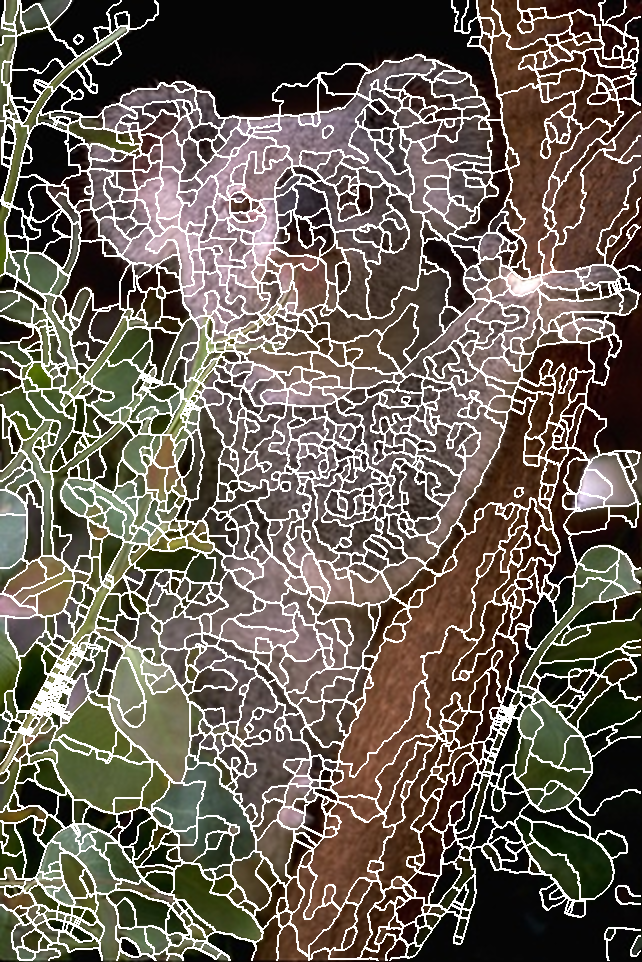
\includegraphics[width=0.25\textwidth]{fig/andres/0.png}
}
\subfloat[Oversegmentation]{  \label{fig:naive_thresholding_b}
    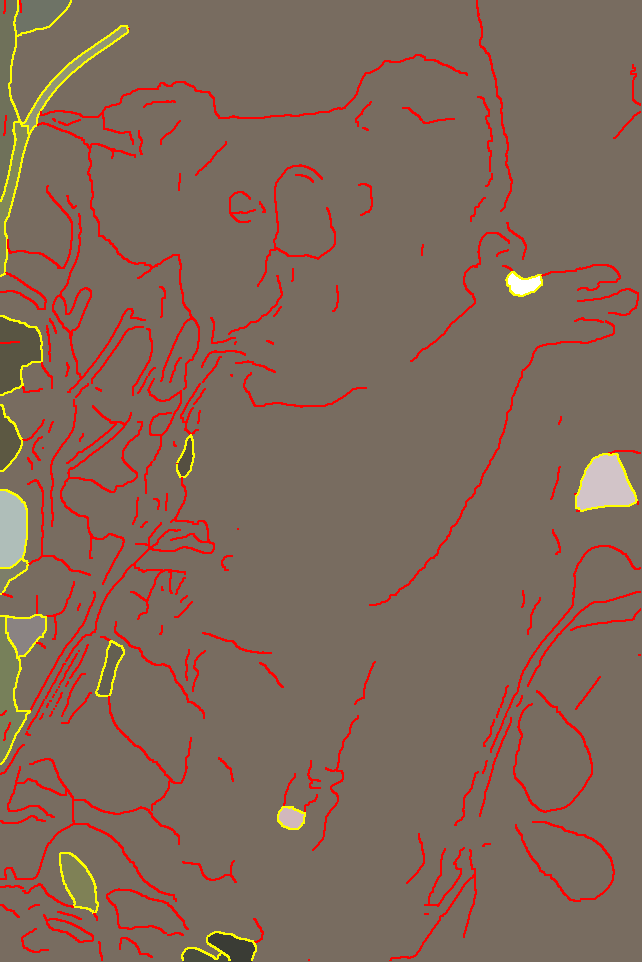
\includegraphics[width=0.25\textwidth]{fig/andres/1.png}
}
\subfloat[Oversegmentation]{  \label{fig:naive_thresholding_c}
    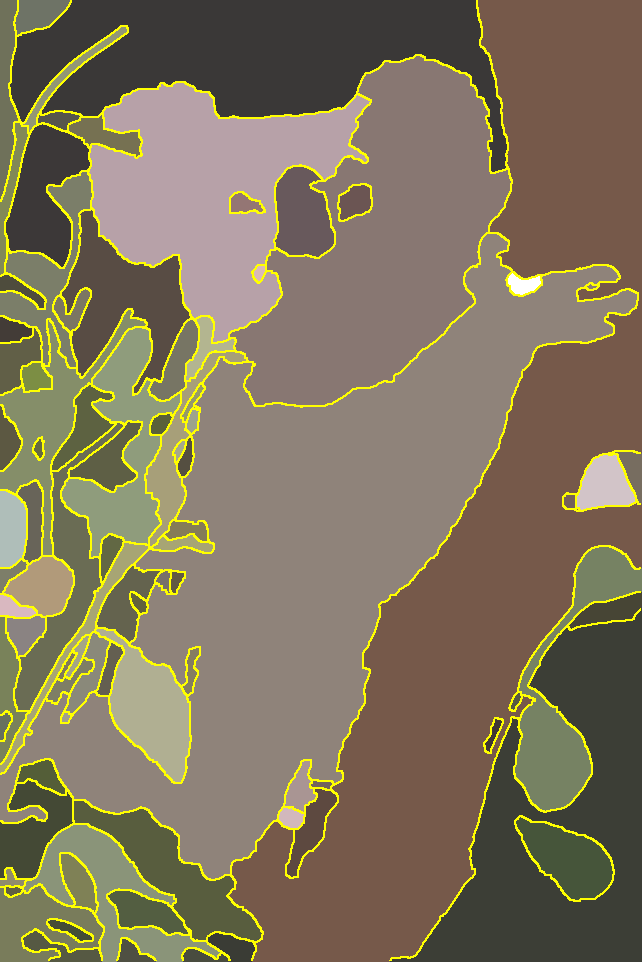
\includegraphics[width=0.25\textwidth]{fig/andres/2.png}
}
\addtocontents{lof}{%
    \vspace{1cm}
    \protect\centerline{%
        \protect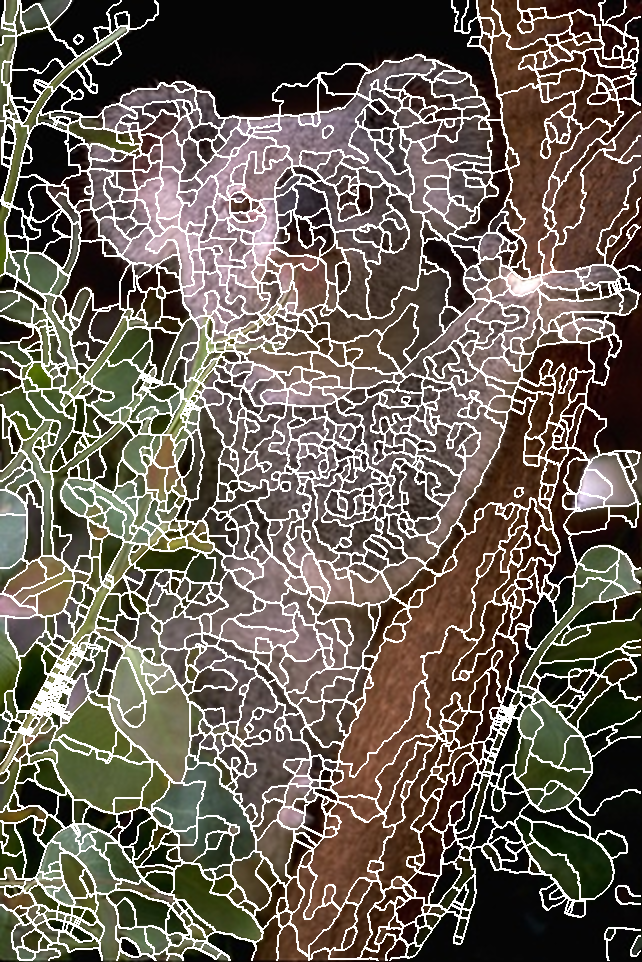
\includegraphics[width=.075\linewidth]{fig/andres/0.png}\hspace{0.2cm}
        \protect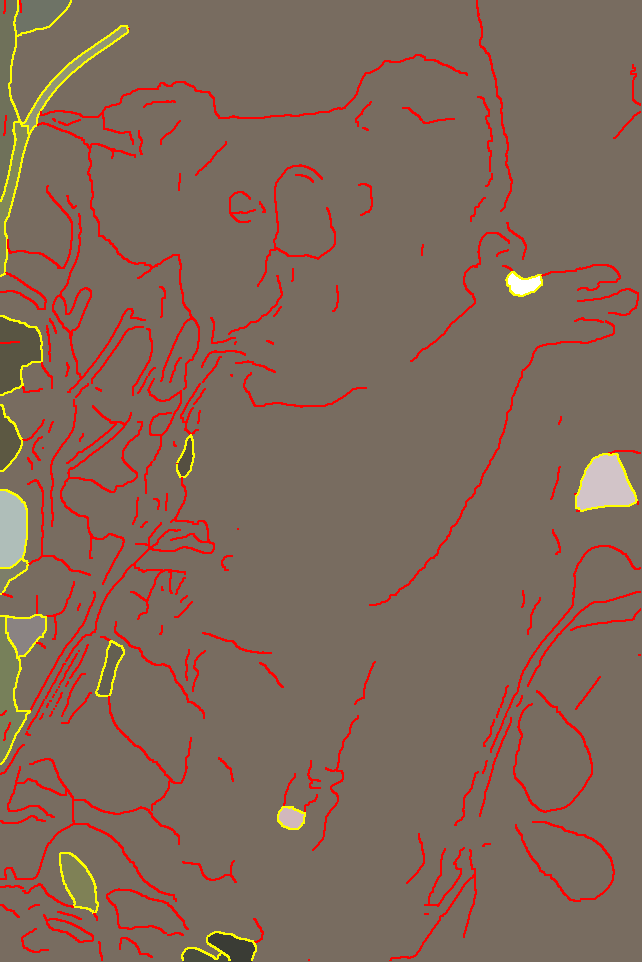
\includegraphics[width=.075\linewidth]{fig/andres/1.png}\hspace{0.2cm}
        \protect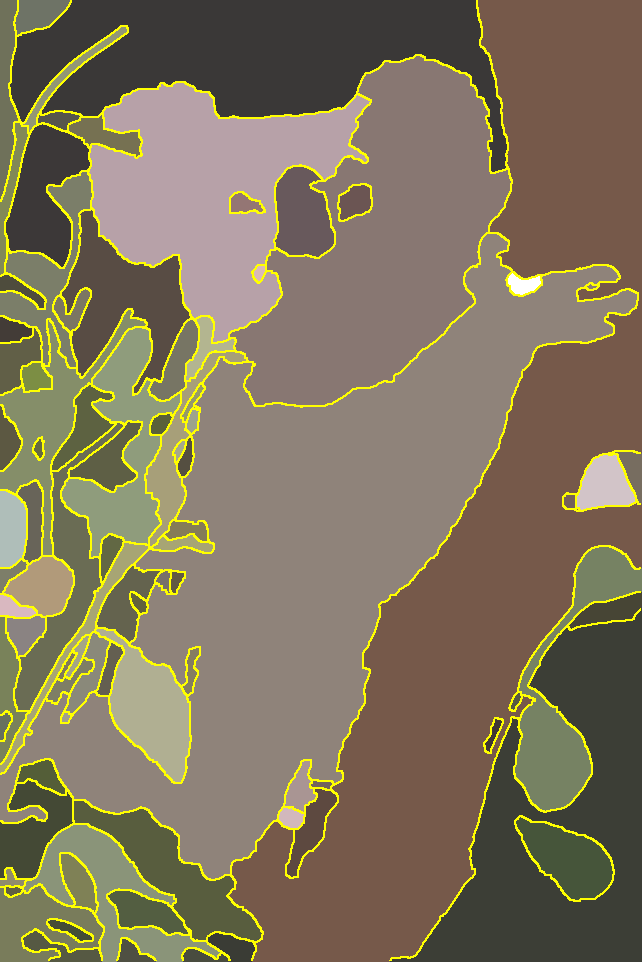
\includegraphics[width=.075\linewidth]{fig/andres/2.png} 
    }%
}%
\caption[Naive thresholding vs. multicuts]{
This figure has been taken from \cite{andres_2011_iccv} .
\Cref{fig:naive_thresholding_a} shows the oversegmentation of 
an image .
\Cref{fig:naive_thresholding_b} shows the result of naive thresholding..
Any inconsistent boundary is shown in red while consistent
boundaries are shown in yellow. 
\Cref{fig:naive_thresholding_c} shows the result with the multicut
constraints which lead to a meaningful segmentation.
} \label{fig:naive_thresholding}
\end{figure}


\citet{andres_2011_iccv} and \citet{kappes_2011_emmcvpr} use a
cutting plane approach where violated constraints are added
iteratively until no more violated constraints are found.


\begin{figure}
\centering
\subfloat[Superpixel Segmentation]{ \label{fig:mc_ineq_0}
    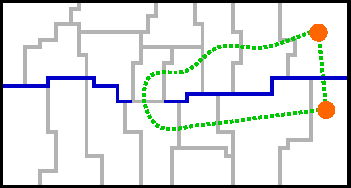
\includegraphics[width=0.4\textwidth]{fig/andres/ineq_0.pdf}
}
\subfloat[Corresponding Graph]{ \label{fig:ineq_1}
    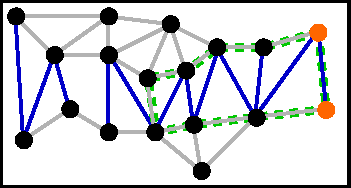
\includegraphics[width=0.4\textwidth]{fig/andres/ineq_1.pdf}
}
\addtocontents{lof}{%
    \vspace{1cm}
    \protect\centerline{%
        \protect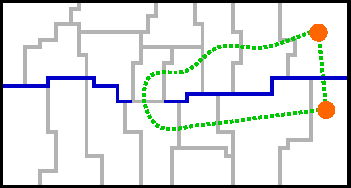
\includegraphics[width=.075\linewidth]{fig/andres/ineq_0.pdf}\hspace{0.2cm}
        \protect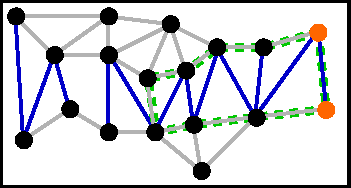
\includegraphics[width=.075\linewidth]{fig/andres/ineq_1.pdf}
    }%
}%
\caption[Violated multicut constraints]{
This figure has been taken from \cite{andres_2011_iccv} .
\Cref{fig:mc_ineq_0} shows the oversegmentation of 
an image .
\Cref{fig:mc_ineq_1} shows the corresponding graph.
} \label{fig:mc_ineq}
\end{figure}

 

%\section{Hierarchical Clustering}\label{sec:rw_hc}
% !TEX root = ../../main.tex
\section{Hierarchical Clustering}\label{sec:rw_hc}

%%%%%%%%%%%%%%%%%%%%%
%dendrogram
%%%%%%%%%%%%%%%%%%%%%%
\begin{figure}[H]
    \centering
    \subfloat[Bottom-Up: Nodes are merged with increasing time]{\label{fig:hc_bottom_up}
        {
            \begin{tikzpicture}[sloped]
                \node (a)    at (-6,0)      {a};
                \node (b)    at (-5,0)      {b};
                \node (c)    at (-4,0)    {c};
                \node (d)    at (-3,0)     {d};
                \node (e)    at (-2,0)       {e};

                \node (ab)   at (-5.5,1)    {};
                \node (cd)   at (-3.5,1)    {};
                \node (cde)  at (-2.75,2)       {};
                \node (all)  at (-4,3)    {};
                
                \node (root) at (-4,4) {root}; 

                \draw (a) |- (ab.center);
                \draw (b) |- (ab.center);
                \draw (c) |- (cd.center);
                \draw (d) |- (cd.center);
                \draw (e) |- (cde.center);
                \draw (cd.center) |- (cde.center);
                \draw (ab.center) |- (all.center);
                \draw (cde.center) |- (all.center);
                \draw (all.center) |- (root.center);

                \draw[->,-triangle 60] (-7,0) -- node[above]{time} (-7,4);
            \end{tikzpicture}
        }
    }\hspace{2cm}
    \subfloat[Top-Down: Nodes are divided with increasing time]{\label{fig:hc_top_down}
        {
            \begin{tikzpicture}[sloped]
                \node (a)    at (-6,0)      {a};
                \node (b)    at (-5,0)      {b};
                \node (c)    at (-4,0)    {c};
                \node (d)    at (-3,0)     {d};
                \node (e)    at (-2,0)       {e};

                \node (ab)   at (-5.5,1)    {};
                \node (de)   at (-2.5,1)    {};
                \node (cde)  at (-3.25,2)       {};
                \node (all)  at (-4,3)    {};
                
                \node (root) at (-4,4) {root}; 

                \draw (a) |- (ab.center);
                \draw (b) |- (ab.center);
                \draw (c) |- (cde.center);
                \draw (d) |- (de.center);
                \draw (e) |- (de.center);        
                \draw (de.center) |- (cde.center);
                \draw (ab.center) |- (all.center);
                \draw (cde.center) |- (all.center);
                \draw (all.center) |- (root.center);

                \draw [->,-triangle 60] (-7,4) -- node[below,align=center]{time} (-7,0);
            \end{tikzpicture}
        }
    }
    \addtocontents{lof}{%
    \vspace{1cm}
    \protect\centerline{%
    \protect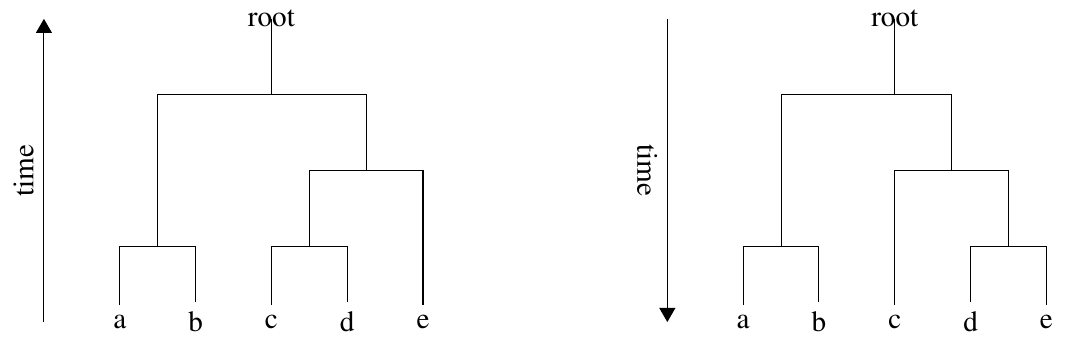
\includegraphics[width=.2\linewidth]{fig/thump/dendro.png}
    }%
    }%
    \caption[Bottom-up vs. top-down hierarchical clustering]{
        Bottom-Up clustering: Nodes are merged with increasing time.
        At the begin, all nodes are leafs, and they are merged
        together.
        Top-Down clustering: Nodes are divided with increasing time.
        At the begin, all nodes are in the root of the tree,
        and with increasing time, nodes are split.

    }
    \label{fig:hc_bottom_up_top_down}
\end{figure}


Hierarchical clustering techniques have been successfully used
in computer vision since decades \citep{ohlander_1978_cgip,forsyth_2002_book,arbelaez_2006_cvpr,iglesias_2013,morel_1995_book}.

The method  of \citet{ohlander_1978_cgip} is an example for \emph{top-down} clustering,
where all pixels start in one single cluster. Each cluster is recursively divided 
into  more clusters. The method proposed in \cref{ch:cgc} has a strong connection to
\emph{top-down} clustering.
\citet{arbelaez_2006_cvpr} and \citet{iglesias_2013} use the bottom-up approach,
also called \emph{agglomerative clustering}, where 
adjacent nodes in a graph are merged iteratively to create 
a set of nested segmentations.


Such a hierarchy of clusters can be visualized as a dendrogram (see \cref{fig:hc_bottom_up_top_down} ).
The dendrogram can be interpreted as a tree where each node represents a
region in the image.
The leafs in the tree are the atomic units of the image (e.g. pixels, super-pixels or super-voxels)
and the root note is the entire scene itself (e.g. the complete image / graph).

There are a few differences between classic unstructured agglomerative clustering
\citep{florek_1951,sokal_1958_science_bulletin,ward_63_jasa}
and agglomerative clustering on graph data structures \citep{arbelaez_2006_cvpr,iglesias_2013,morel_1995_book}, 
e.g. grid-graphs and region adjacency graphs\citep{vlachos_1993_csv}.
While in unstructured hierarchical clustering, any pair of observations can be merged,
for graph hierarchical clustering, only adjacent nodes / regions can be merged.
In the literature this is also called ``hierarchical clustering with connectivity constraints'' \cite{scikit_learn}.


The main idea behind agglomerative clustering is very simple:

Initially, all observations start in a single cluster. 
Next, clusters which have highest similarities will be merged
iteratively.
Due to this merging, similarities change and need to be updated
/ recomputed. Therefore  noisy initial features
 become more informative.


\begin{table}
\begin{scriptsize}
\begin{tabular}{ |l|l|p{5cm}|}
    \hline 
    Euclidean Distance
        & $||a-b||_2 = \sqrt{\sum{ (a_i-b_i })^2 } $
        & For low dimensional data \\  \hline 
    Squared Euclidean Distance
        & $||a-b||_2^2 = \sum{ (a_i-b_i })^2  $
        & For low dimensions data\\  \hline
    Manhattan Distance
        &  $||a-b||_1 = \sum{ |a_i-b_i |}  $
        & Multi purpose \\  \hline 
    $\mathcal{X}^2$-Distance  
        &  $\frac{1}{2}\sum{  \frac{(a_i-b_i)^2}{a_i+b_i} }$
        & For histograms \\  \hline 
    Earth Mover  Distance          
        &  see \citet{levina_2001_iccv} 
        & For histograms \\  \hline 

\end{tabular}

\end{scriptsize}
\caption{
    An overview of the most common distances measurements and their main properties.
}\label{tab:hc_distance_types}
\end{table}



\begin{table}
\begin{scriptsize}
\begin{tabular}{ |l|l|p{5cm}|}
    \hline
    Average Linkage \citep{sokal_1958_science_bulletin}           
        & $d_{al}(C_a,C_b) = \frac{1}{|C_a||C_b|} \sum _{a \in C_a} \sum_{b \in C_b} d(a,b) $ 
        & \scriptsize Prefers clusters with same variance \cite{sokal_1958_science_bulletin} \\ \hline

    Single Linkage \citep{florek_1951}            
        & $d_{sl}(C_a,C_b) =  \min\{d(a,b) : a \in C_a, b \in C_b\}$ 
        & Nice theoretic properties \citep{hartigan_1981_jjamstat,milligan_1980_psycho}, can lead
          to very irregular shaped clusters \\ \hline
    Complete Linkage \citep{sorensen_1948}         
        & $d_{cl}(C_a,C_b) =  \max\{d(a,b) : a \in C_a, b \in C_b\}$ 
        & Prefers clusters with same diameter \citep{milligan_1980_psycho} \\ \hline
    Centroid Distance         
        & $d_{cd}(C_a,C_b) =  d(\bar{C}_a,\bar{C}_b) $ 
        & Robust w.r.t. outliers \citep{milligan_1980_psycho} \\ \hline
    Wards Minimum Variance \citep{ward_63_jasa}
        & $d_{wmv}(C_a,C_b) = \frac{ d(\bar{C}_a,\bar{C}_b)}{ \frac{1}{|C_a|} + \frac{1}{|C_b|} } $ 
        & Prefers clusters with same size, is sensible to outliers \citep{milligan_1980_psycho} \\ \hline
\end{tabular}

\end{scriptsize}

\caption{
    The distance between to clusters is usually based on the 
    individual distance between elements within the clusters.
    These distance are \emph{linked} together.
    An overview of the most common cluster distances linkages and their main properties.
}\label{tab:hc_linkage_types}
\end{table}


The definition of a specific distance betweens clusters is crucial, 
but strongly depends on the application.
The distance between two clusters is usually based on the 
individual distance between elements within the clusters.
These distance are then \emph{linked} together using a specific linkage type.
\Cref{tab:hc_distance_types} gives a short overview of many common distance
types and \cref{tab:hc_linkage_types} gives a  brief overview 
of most common cluster linkage types and their main properties.








\iffalse
\begin{tikzpicture}[scale=  1,every node/.style={minimum size=1cm},on grid]
        
    %slanting: production of a set of n 'laminae' to be piled up. N=number of grids.
    

    %%%%%%%%%%%%%%%%%%%%%%%%%%%%%%%%%%%%%%%%%%%%%%%%%%%%%%%%%%%%%%%
    % 0 bottom layer
    %%%%%%%%%%%%%%%%%%%%%%%%%%%%%%%%%%%%%%%%%%%%%%%%%%%%%%%%%%%%%%%%
        
    \begin{scope}[yshift=0,every node/.append style={yslant=0.5,xslant=-1},yslant=0.5,xslant=-1]
        \draw[-latex,thick] (-0.17,3.21/2) node[right]{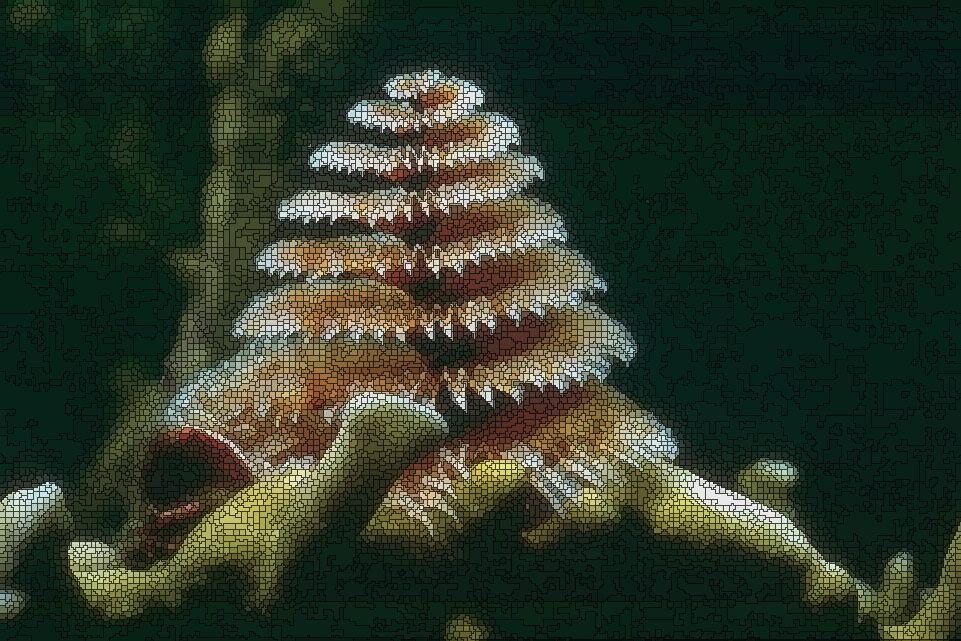
\includegraphics[width=4.82cm]{fig/12074/0.png}};
        \draw[black,very thick] (0,0) rectangle (4.81,3.21);
    \end{scope}

    \begin{scope}[yshift=60*1,every node/.append style={yslant=0.5,xslant=-1},yslant=0.5,xslant=-1]
        \draw[-latex,thick] (-0.17,3.21/2) node[right]{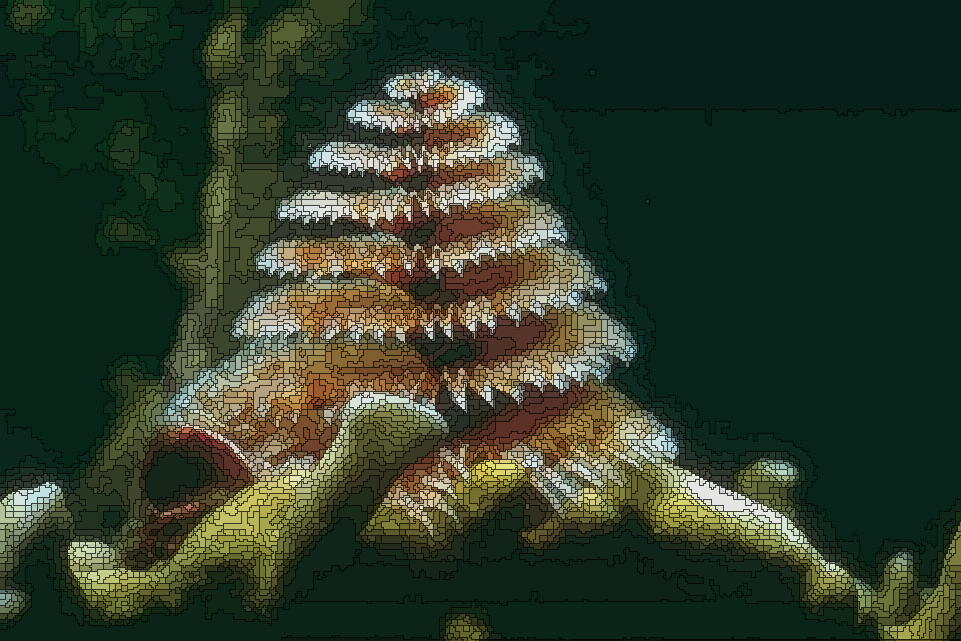
\includegraphics[width=4.82cm]{fig/12074/2.png}};
        \draw[black,very thick] (0,0) rectangle (4.81,3.21);
    \end{scope}

    \begin{scope}[yshift=60*2,every node/.append style={yslant=0.5,xslant=-1},yslant=0.5,xslant=-1]
        \draw[-latex,thick] (-0.17,3.21/2) node[right]{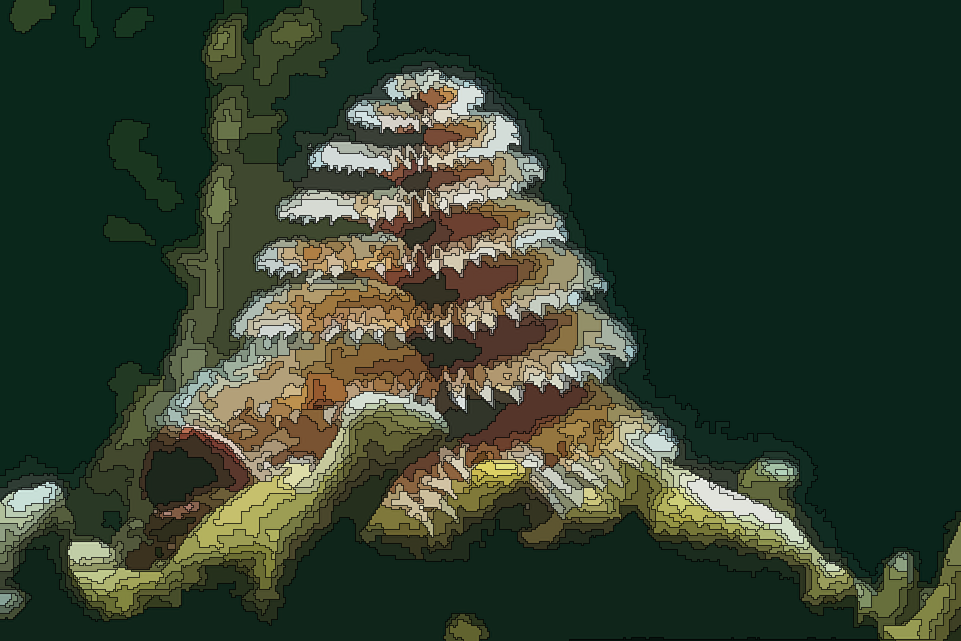
\includegraphics[width=4.82cm]{fig/12074/4.png}};
        \draw[black,very thick] (0,0) rectangle (4.81,3.21);
    \end{scope}

    \begin{scope}[yshift=60*3,every node/.append style={yslant=0.5,xslant=-1},yslant=0.5,xslant=-1]
        \draw[-latex,thick] (-0.17,3.21/2) node[right]{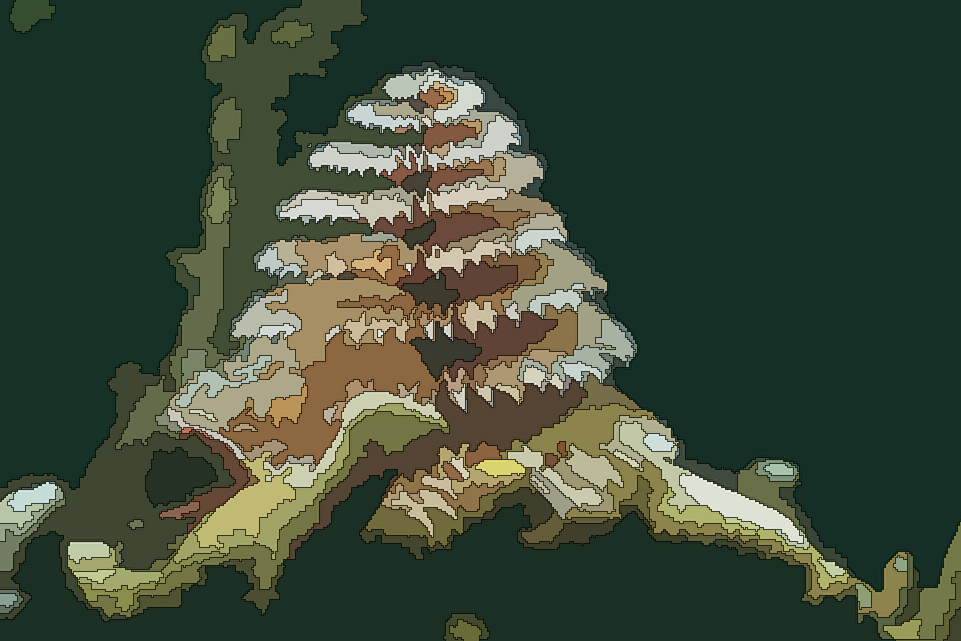
\includegraphics[width=4.82cm]{fig/12074/6.png}};
        \draw[black,very thick] (0,0) rectangle (4.81,3.21);
    \end{scope}

    \begin{scope}[yshift=60*4,every node/.append style={yslant=0.5,xslant=-1},yslant=0.5,xslant=-1]
        \draw[-latex,thick] (-0.17,3.21/2) node[right]{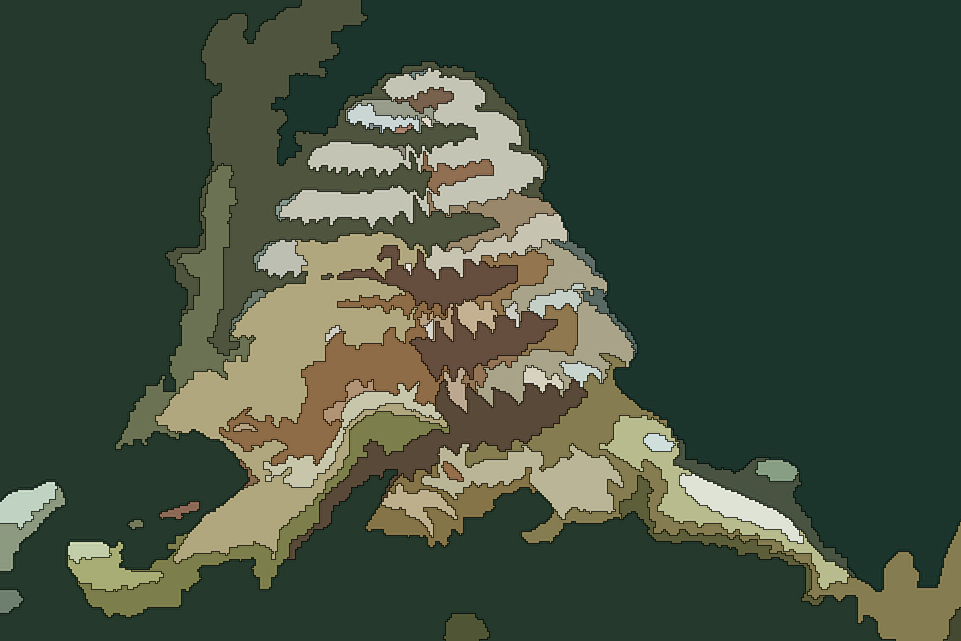
\includegraphics[width=4.82cm]{fig/12074/8.png}};
        \draw[black,very thick] (0,0) rectangle (4.81,3.21);
    \end{scope}


    \draw[->,-triangle 60] (-3,0) -- node[above]{time} (-3,4);

    %%%%%%%%%%%%%%%%%%%%%%%%%%%%%%%%%%%%%%%%%%%%%%%%%%%%%%%%%%%%%%%
    % 0 bottom layer
    %%%%%%%%%%%%%%%%%%%%%%%%%%%%%%%%%%%%%%%%%%%%%%%%%%%%%%%%%%%%%%%%
    \draw[-latex,thick] (6.2,2) node[right]{$\mathsf{over-segmentation}$}
         to[out=180,in=90] (4,2);
         
         
         
    %%%%%%%%%%%%%%%%%%%%%%%%%%%%%%%%%%%%%%%%%%%%%%%%%%%%%%%%%%%%%%%
    % 1 layer
    %%%%%%%%%%%%%%%%%%%%%%%%%%%%%%%%%%%%%%%%%%%%%%%%%%%%%%%%%%%%%%%%
    
    \draw[-latex,thick] (6.2,5.5) node[right]{$\mathsf{Region adjacency graph 1}$}
         to[out=180,in=90] (4,5.5);
\end{tikzpicture}
\fi







In the case of graph hierarchical clustering, informative features
can also be attached to the edges of the graph.
Edge detectors such as the gradient magnitude, gPb \citep{marie_2008_cvpr}  or learned
edge detectors \cite{dollar_2013_iccv}  can be used to boost performance
of agglomerative clustering \citep{arbelaez_2006_cvpr,iglesias_2013}.


\citet{ arbelaez_2006_cvpr} introduce the following notation:
They use $\Omega \in \mathbb{R}^2$ as image domain.
$P_0$ is the initial partition and they define a
\emph{hierarchical segmentation operator} (HSO) which
assigns a partition $P_\lambda$ given the initial partition and
a scale parameter $\lambda$.
Furthermore the following properties must be fulfilled for a HSO:  

\begin{align} 
P_{\lambda}  =  P_0 ,\hspace{0.5cm}  \forall \lambda \leq 0  \label{eq:ucm_hco_eq_0} \\ 
\exists \lambda_1 \in \mathbb{R}^+  : P_{\lambda}  =  \{ \Omega \} ,\hspace{0.5cm} \forall \lambda \geq \lambda_1  \label{eq:ucm_hco_eq_1} \\
\lambda < \lambda'  \rightarrow  P_{\lambda} \sqsubseteq   P_{\lambda'} \label{eq:ucm_hco_eq_2}
\end{align}


\Cref{eq:ucm_hco_eq_0} and \cref{eq:ucm_hco_eq_1}  give $\lambda$ a range.
\Cref{eq:ucm_hco_eq_2} ensures that the segmentations are nested.
They define the \emph{saliency} of a contour as the scale $\lambda$ where
the contour disappears (see \cref{fig:ucm_visu}).
Thresholding the saliency map leads to closed contours.
As a consequence, the complete hierarchical segmentation
generated by a HSO can be encoded in the saliency map (see \cref{fig:ucm_saliency}).


\citet{iglesias_2013} improve segmentation results by combining 
agglomerative clustering combined machine learning.
Their main idea is to combine training data at multiple scales
which are generated during the region merging process.
This approach outperforms single scale learning.


\begin{figure} 
    \begin{center}
        \subfloat[$K_0$]{ \label{fig:ucm_k0}
            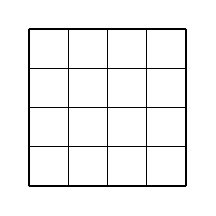
\begin{tikzpicture}
                \draw[step=0.5,black,thin] (0.0,0.0) grid (2,2);
                \draw[step=2,black,thick] (0.0,0.0) grid (2,2);
            \end{tikzpicture}
        }
        \hspace{0.5cm}
        %
        %
        %
        \subfloat[$K_1$]{ \label{fig:ucm_k1}
            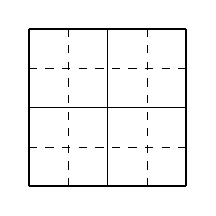
\begin{tikzpicture}
                \draw[step=0.5,black,very thin,dashed] (0.0,0.0) grid (2,2);
                \draw[step=1,black,thin] (0.0,0.0) grid (2,2);
                \draw[step=2,black,thick] (0.0,0.0) grid (2,2);
            \end{tikzpicture}
        }
        \hspace{0.5cm} 
        %
        %
        %
        \subfloat[$K_2$]{\label{fig:ucm_k2}
            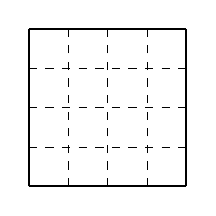
\begin{tikzpicture}
                \draw[step=0.5,black,very thin,dashed] (0.0,0.0) grid (2,2);
                \draw[step=2,black,thick] (0.0,0.0) grid (2,2);
            \end{tikzpicture}
        }
        \hspace{0.5cm}
        %
        %
        %
        \subfloat[$\mathcal{C}(\Upsilon) $]{ \label{fig:ucm_saliency}
            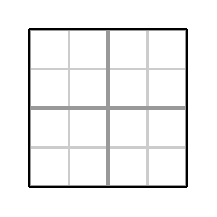
\begin{tikzpicture}
                \draw[step=0.5,black!20,thick] (0.0,0.0) grid (2,2);
                \draw[step=1,  black!40,very thick] (0.0,0.0) grid (2,2);
                 \draw[step=2,black,thick] (0.0,0.0) grid (2,2);
            \end{tikzpicture}
        }
        \hspace{0.5cm}
        %
        %
        %
        \subfloat[$\mathcal{C}(\Upsilon) $]{ \label{fig:ucm_saliency_3d}
            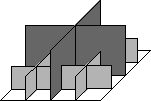
\includegraphics[width=0.2\textwidth]{fig/ucm3d.pdf}
        }
    \end{center}
    \addtocontents{lof}{%
    \vspace{1cm}
    \protect\centerline{%
        \protect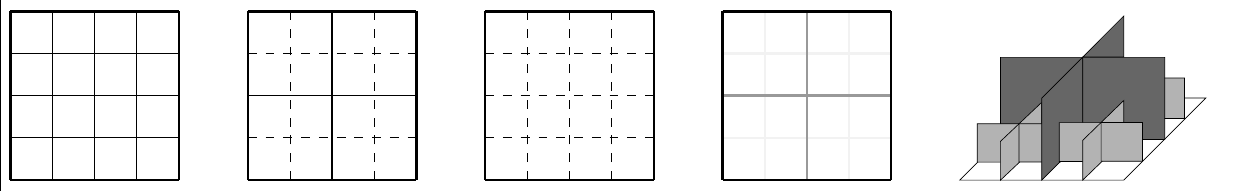
\includegraphics[width=.2\linewidth]{fig/thump/ucm.png} 
    }%
    }%
    \caption[Ultra metric contour map saliency]{
        \Cref{fig:ucm_k0} shows the a $4x4$ grid graph which serves as initial segmentation $K_0$.
        \Cref{fig:ucm_k1} shows the segmentation $K_1$ after the contraction of a few edges.
        Contracted edges are shown dashed.
        \Cref{fig:ucm_k2} shows the graph after all edges have been contracted.
        \Cref{fig:ucm_saliency} shows the saliency $\mathcal{C}$ of the contour $\Upsilon$.
        In \cref{fig:ucm_saliency_3d} the saliency from \ref{fig:ucm_saliency} is
        showed as a 3D visualization.
        This figure is very much inspired by \citep{arbelaez_2006_cvpr}.
    }\label{fig:ucm_visu}
\end{figure}




\Citet{najman_1994_sp} showed that there is a
strong connection between hierarchical segmentations
and watersheds.
They prove that there exists a bijection between
the set of ultrametric watersheds\citep{najman_2010_corr} and the set of hierarchical segmentations.
Furthermore, a recursive application of the watershed transformation  can
be used to generate a hierarchy of nested segmentations.
This transformation is called \emph{waterfall transformation} \citep{beuchner_1994_waterfall} .
 

%\section{Watershed Methods}\label{sec:rw_watershed_methods}
% !TEX root = ../../main.tex
\section{Watershed Methods}\label{sec:rw_watershed_methods}

The idea of watersheds has been introduced by \citet{beucher_1979_workshop}.

Other watersheds \citep{vinent_1991_pami,najman_1994_sp,roerdink_2000_finf,bertrand_2005_jmiv,cousty_2009_pami}.


The watershed algorithm can be often described with the following analogy:

\paragraph{Water Flooding:} A grayscale  image can be interpreted as hight map (see \cref{fig:ws_2d_map}, \cref{fig:ws_2d_map3d}).
The water level is raised as shown in \cref{fig:ws_a} - \cref{fig:ws_f}.
A watershed is wherever the water of two adjacent valleys is meeting (see \cref{fig:ws_e},\cref{fig:ws_f} and \cref{fig:ws_2d_lines}).


% watersheds illustrated
\begin{figure}
    \centering
    \subfloat[1d Image Data]{ \label{fig:ws_a}
        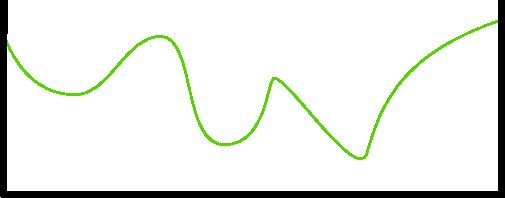
\includegraphics[width=0.25\textwidth]{fig/ws_no_no.pdf}
    }
    \hspace{0.5cm}
    \subfloat[Local minima]{  \label{fig:ws_b}
        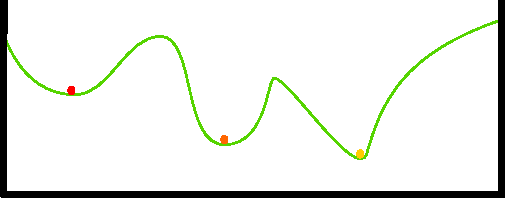
\includegraphics[width=0.25\textwidth]{fig/ws_no.pdf}
    }
    \hspace{0.5cm}
    \subfloat[flooding starts]{  \label{fig:ws_c}
        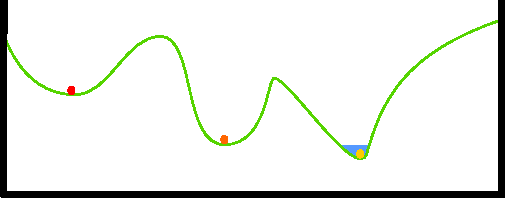
\includegraphics[width=0.25\textwidth]{fig/ws3.pdf}
    }
    \\
    \subfloat[flooding]{  \label{fig:ws_d}
        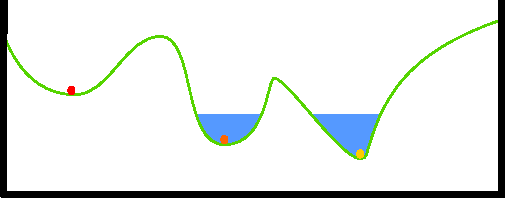
\includegraphics[width=0.25\textwidth]{fig/ws2.pdf}
    }
    \hspace{0.5cm}
    \subfloat[watershed 1]{  \label{fig:ws_e}
        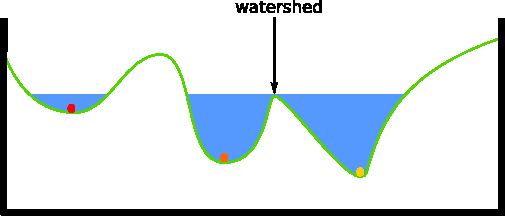
\includegraphics[width=0.25\textwidth]{fig/ws1.pdf}
    }
    \hspace{0.5cm}
    \subfloat[watershed 2]{ \label{fig:ws_f}
        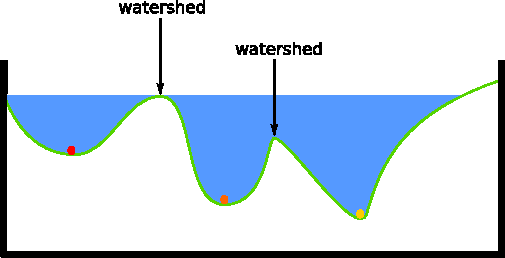
\includegraphics[width=0.25\textwidth]{fig/ws0.pdf}
    }
    \\ % 2D Watersheds
    \subfloat[$ $]{ \label{fig:ws_2d_map}
        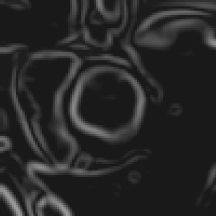
\includegraphics[height=0.26\textwidth]{fig/ws2d0.png}
    }
    \hspace{0.1cm}
    \subfloat[$ $]{ \label{fig:ws_2d_map3d}
        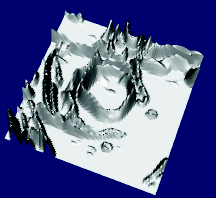
\includegraphics[height=0.26\textwidth]{fig/ws2d1.png} 
    }
    \hspace{0.1cm}
    \subfloat[$ $]{ \label{fig:ws_2d_lines}
        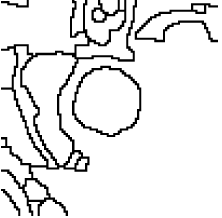
\includegraphics[height=0.26\textwidth]{fig/ws2d2.png}
    }

    \addtocontents{lof}{%
        \vspace{1cm}
        \protect\centerline{%
            \protect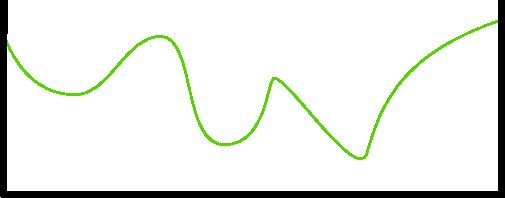
\includegraphics[width=.075\linewidth]{fig/ws_no_no.pdf}  \hspace{0.2cm}
            \protect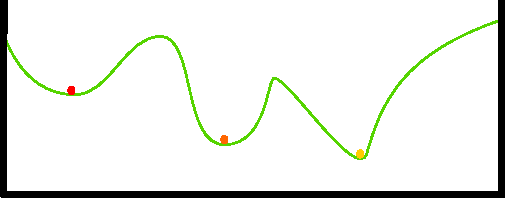
\includegraphics[width=.075\linewidth]{fig/ws_no.pdf}\hspace{0.2cm}
            \protect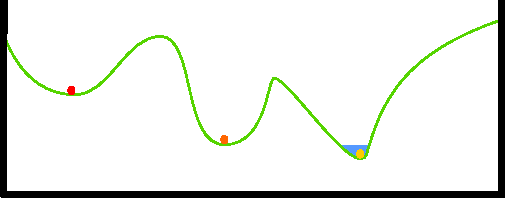
\includegraphics[width=.075\linewidth]{fig/ws3.pdf} 
        }%
        \vspace{0.2cm}
        \protect\centerline{%
            \protect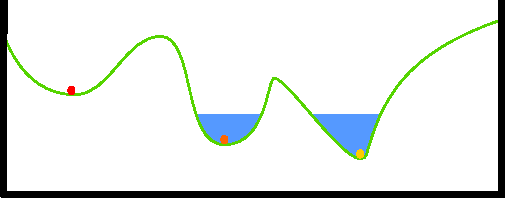
\includegraphics[width=.075\linewidth]{fig/ws2.pdf}  \hspace{0.2cm}
            \protect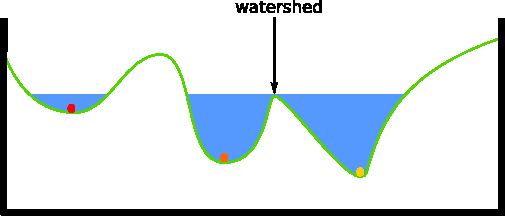
\includegraphics[width=.075\linewidth]{fig/ws1.pdf} \hspace{0.2cm}
            \protect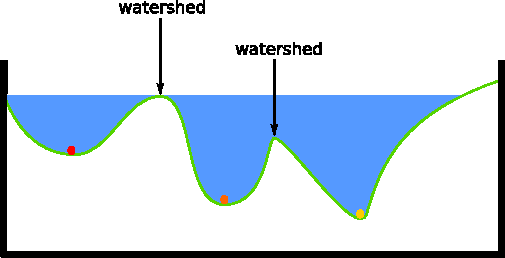
\includegraphics[width=.075\linewidth]{fig/ws0.pdf}%
        }%
        \vspace{0.2cm}
        \protect\centerline{%
            \protect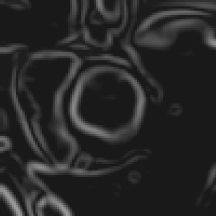
\includegraphics[height=.075\linewidth]{fig/ws2d0.png}  \hspace{0.2cm}
            \protect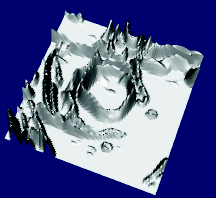
\includegraphics[height=.075\linewidth]{fig/ws2d1.png} \hspace{0.2cm}
            \protect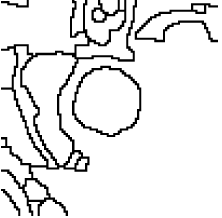
\includegraphics[height=.075\linewidth]{fig/ws2d2.png}%
        }%
    }%
    \caption[Illustration of watershed flooding process]{ 
        Illustration of watershed flooding process.
        The water level raises, and the watersheds are at the positions where water from different catchment basins is meeting.
    } \label{fig:watersheds_1d}
\end{figure}





\citet{couprie_2011_pami} proposed an algorithm, \emph{power-watershed}, a generalization of \citep{RANDOM_WALKER, boykov_2001_pami,vinent_1991_pami,najman_1994_sp,roerdink_2000_finf,bertrand_2005_jmiv,sinop_2007_iccv,cousty_2009_pami}.

They define the following model.
\begin{align}\label{eq:power_watershed}
\min_x \sum_{e_{ij} \in E}  w_{ip}^p |x_i-x_j|^q + \sum_{v_i } w_{Fi}^p |x_i|^q + \sum_{v_i } w_{Bi}^p |x_i-1|^q \\
s.t. \hspace{0.35cm} x(F)=1, \hspace{0.5cm} x(B)=0
\end{align}
Setting $p$ to 1 will lead to the methods proposed by \citet{sinop_2007_iccv}.
\Citet{allene_icv_2010} pointed out when $p=1$ and $q \rightarrow \infty$, solving
\cref{eq:power_watershed} is equivalent to applying a minimum spanning forest algorithm.




\citet{straehle_2011_miccai} proposed a watershed based method for interactive segmentation
of neural volume electron  microskopy images.
They show how a background prior be be efficiently integrated into watersheds,
and that this prior is beneficial for neuro data.
In addition \citet{straehle_2012_cvpr} proposed an uncertainty estimator for
guided interactive segmentation based on watersheds.
 

%\section{Energy Based Methods}\label{sec:energy_based_methods}
% !TEX root = ../../main.tex
\section{Energy Based Methods}\label{sec:energy_based_methods}

Energy based methods have recently become very popular.

Given a graph $G = (E,V)$ we 
associate  a variable $ x_i \quad \forall  u_i \in V$ with every node.
Within this thesis we focus on discrete energy functions,
therefore we use discrete variables $x$.
W.l.o.g. we set  $ x_i   \in \{ 0,1,2,\ldots, N_{labels}-1 \} \quad \forall \quad u_i \in V$,
which means that any node has the same number of labels.

An energy function $E(x)$ can be  defined  in the following way:

\begin{equation} \label{eq:gm_energy}
    E(x) = 
    \underbrace{
        \sum_{v \in V} \phi_i(x_i)
    }_{\text{unaries}}
     \quad +  \quad
    \underbrace{
        \sum_{e=(i,j) \in E } \phi_{ij}(x_i,x_j) 
    }_{\text{pairwise terms}}
\end{equation}



Here the \emph{unaries} $\phi_i(x_i)$ encode local costs
for a variable to have a certain label.
The \emph{pairwise terms} $\phi_{ij}(x_i,x_j) $ define the interaction of adjacent nodes.
Often they are used to introduce some smoothness prior
into the model \citep{szeliski_2008_pami}.
The vector which yields a minimum value of $E(x)$
is called $x_{\text{optimal}}$.
\begin{equation} \label{eq:gm_argmin}
x_{\text{optimal}} = \argmin_{x}  E(x)
\end{equation}

Before discussing how to optimize such energy functions,
we will give some concrete examples how $E(X)$ 
can be defined.



\paragraph{Denoising:}


Let $G=(V,E)$ be a grid graph corresponding to
a grayscale image.
Setting $N_{labels}$ to $256$ we can interpret  the variables $x$ directly as
gray values.
Let $I_i$ be the gray value of the pixel associated with variable $x_i$.

\begin{equation} \label{eq:gm_ef_dension}
E(x) = \sum_{v \in V}  (I_i - x_i)^2 + \sum_{e=(i,j) \in E } \lambda (x_i-x_j)^2
\end{equation}

The unaries ensure that the labeling matches the image.
The second order terms penalize adjacent nodes where the difference
between the labels is huge.
This model is described as part of a collection of MRF benchmark models \citep{szeliski_2008_pami}.




\begin{figure}[H]
    \centering
    \subfloat[Input Image $I$]{ \label{fig:eq:gm_ef_dension_input}
        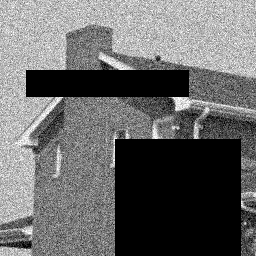
\includegraphics[width=0.25\textwidth]{fig/houseM-input.png}
    }
    \subfloat[ICM]{ \label{fig:eq:gm_ef_dension_icm}
        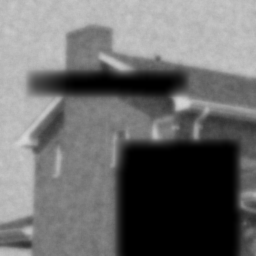
\includegraphics[width=0.25\textwidth]{fig/houseM-ICM.png}
    }
    \subfloat[$\alpha$-Expansion]{  \label{fig:eq:gm_ef_dension_ae}
        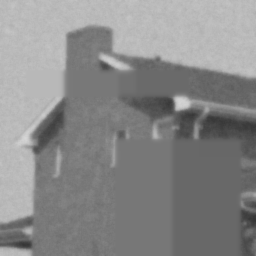
\includegraphics[width=0.25\textwidth]{fig/houseM-Expansion.png}
    }
    \subfloat[TRWS]{  \label{fig:eq:gm_ef_dension_trws}
        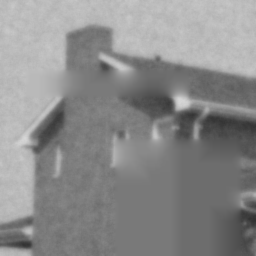
\includegraphics[width=0.25\textwidth]{fig/houseM-TRW-S.png}
    }
    \caption[Energy based truncated denoising]{
        Finding $x_{\text{optimal}} $ for the energy function given
        in \cref{eq:gm_ef_dension} is NP-hard. We show results of approximative solvers.
        Using \cref{fig:eq:gm_ef_dension_input} as input (for the black area no unaries 
        are used)
        the following
        results are obtained:
        ICM
         \citep{besag_1986_icm} (\Cref{fig:eq:gm_ef_dension_icm}) fails
        to fill the in-painting area. 
        While TRWS
        \citep{kolmogorov_2006_pami_trws}  (\Cref{fig:eq:gm_ef_dension_trws}) 
        and $\alpha$-Expansion
        \citep{boykov_2001_pami} (\Cref{fig:eq:gm_ef_dension_ae}) 
        can fill the in-painting area
        with meaningful values.
        The input image has been taken from \citep{szeliski_2008_pami}.
        The result images have been generated with OpenGM \citep{andres_2012_opengm_arxiv}.
    }\label{fig:gm_ef_denoise}
\end{figure}




\paragraph{Truncated Denoising:} 

This model is almost the same as the \emph{Denoising} model defined above,
but the second order term is clipped to $\gamma$ if $(x_i-x_j)^2$ is larger than $\gamma$.
Therefore one only pays $\gamma$ at strong edges.
Due to this truncation, the model allows for sharp edges.
This model is also described in \citep{szeliski_2008_pami}.


\begin{equation} \label{eq:gm_ef_dension_truncated}
E(x) = \sum_{v \in V}  (I_i - x_i)^2 + \sum_{e=(i,j) \in E } \lambda \cdot \min\left( (x_i-x_j)^2, \gamma\right)
\end{equation}

\begin{figure}[H]
    \centering
    \subfloat[Input Image $I$]{ \label{fig:eq:gm_ef_dension_truncated_input}
        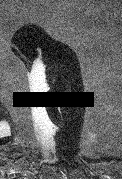
\includegraphics[width=0.25\textwidth]{fig/penguin-bar.png}
    }
    \subfloat[ICM]{ \label{fig:eq:gm_ef_dension_truncated_icm}
        
\includegraphics[width=0.25\textwidth]{fig/penguin-ICM.png}
    }
    \subfloat[$\alpha$-Expansion]{  \label{fig:eq:gm_ef_dension_truncated_ae}
        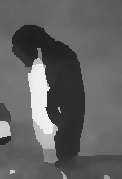
\includegraphics[width=0.25\textwidth]{fig/penguin-Expansion.png}
    }
    \subfloat[Trws]{  \label{fig:eq:gm_ef_dension_truncated_trws}
        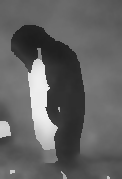
\includegraphics[width=0.25\textwidth]{fig/penguin-TRW-S.png}
    }
    \caption[Energy based truncated denoising]{
        Finding $x_{\text{optimal}} $ for the energy function given
        in \cref{eq:gm_ef_dension_truncated} is NP-hard. We show result of approximative solvers.
        Using \cref{fig:eq:gm_ef_dension_truncated_input} as input (for the black area no unaries 
        are used)
        the following
        results are obtained: ICM \citep{besag_1986_icm}  (\Cref{fig:eq:gm_ef_dension_truncated_icm}) fails
        to fill the in-painting area. While TRWS \cite{kolmogorov_2006_pami_trws}  (\Cref{fig:eq:gm_ef_dension_truncated_trws} ) 
        and $\alpha$-expansion \cite{boykov_2001_pami} (\Cref{fig:eq:gm_ef_dension_truncated_ae}) can fill the in-painting area
        with meaningful values.
        The input image has been taken from \citep{szeliski_2008_pami}.
        The result images have been generated with OpenGM\citep{andres_2012_opengm_arxiv}.
        In contrast to the result of \cref{eq:gm_ef_dension}, this model
        allows sharp edges.
    }\label{fig:gm_ef_dension_truncated}
\end{figure}


\paragraph{Ferromagnetic Ising model}
The ferromagnetic ising model consists 
of binary variables.
The unaries encode local costs for a variable
to take label $0$ or $1$.
The pairwise term is a smoothness prior, which penalizes
adjacent variables with different states.

\begin{equation} \label{eq:gm_ising}
    E(x) = 
    \underbrace{
        \sum_{v \in V} \phi_i(x_i)
    }_{\text{unaries}}
     \quad +  \quad
    \underbrace{
        \beta \cdot \sum_{e=(i,j) \in E }  \delta(\cdot x_i\neq x_j) 
    }_{\text{pairwise potts terms}} ,
\end{equation}
where $\delta(a)=1$ if $a$ is true and $0$ else
and $\beta>0$.

This model is also known as the \emph{potts model} and is often
used for binary segmentation (\eg\quad foreground background segmentation)
but can also be extended to the multi-label case.
Instead of a single $\beta$, often a different $\beta_i$ is used
for each edge \citep{szeliski_2008_pami}.



\begin{figure}[H]
    \centering
    \subfloat[Input Image $I$]{ \label{fig:eq:gm_ef_ising_input}
        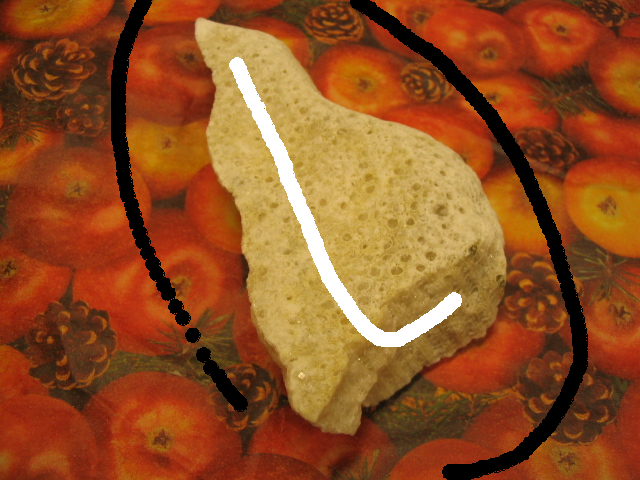
\includegraphics[width=0.25\textwidth]{fig/sponge.png}
    }
    \subfloat[ICM]{ \label{fig:eq:gm_ef_ising_icm}
        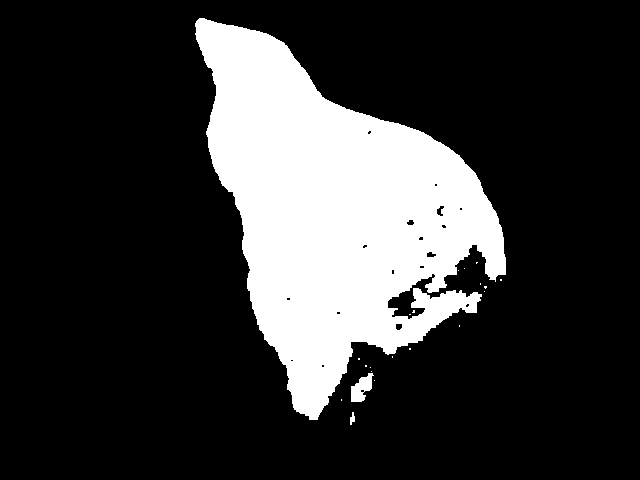
\includegraphics[width=0.25\textwidth]{fig/s_icm.png}
    }
    \subfloat[BP]{  \label{fig:eq:gm_ef_ising_bp}
        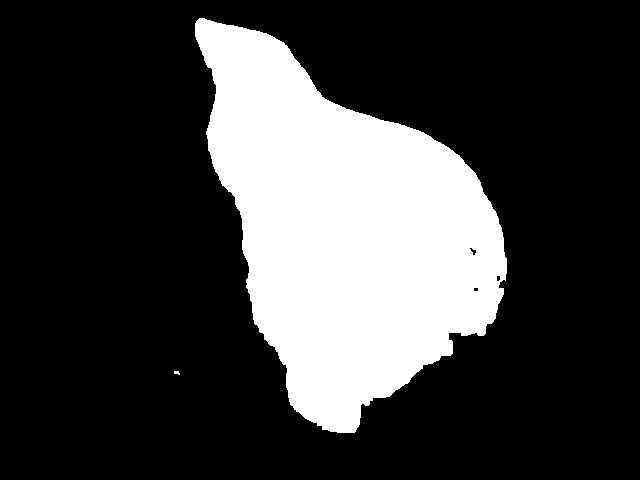
\includegraphics[width=0.25\textwidth]{fig/s_bp.png}
    }
    \subfloat[Graph Cut]{  \label{fig:eq:gm_ef_ising_cg}
        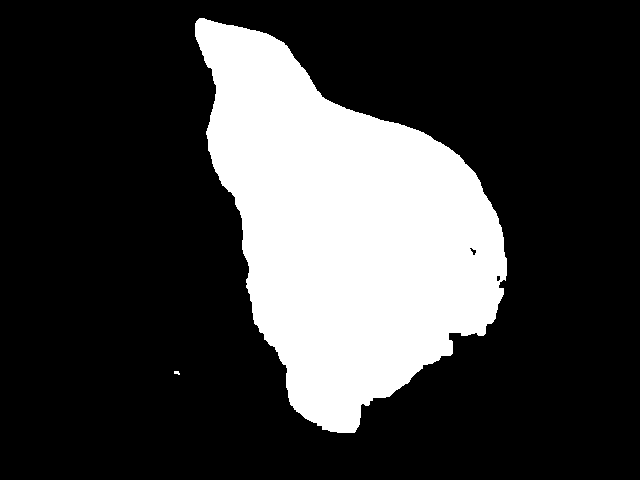
\includegraphics[width=0.25\textwidth]{fig/s_gc.png}
    }
    \caption[Potts Model]{ \label{fig:gm_ef_ising}
        Optimization results for the potts / ising model.
        A grid graph 4-neighborhood is used as input graph and 
        \cref{fig:eq:gm_ef_ising_input} shows the corresponding image.
        The unaries are based on a Gaussian mixture color models of foreground and background seeds defined by the user.
        The potts regularizer is modulated with the local constract.
        Since the model is submodular, graph cut finds optimal solutions (see \cref{sec:gcbased}).
    }
\end{figure}





\paragraph{Multicut Energy Function:}


Segmentation is an important problem in computer vision as a first step
towards understanding an image. Many algorithms start with an over-segmentation
into superpixels, which are then clustered into ``perceptually meaningful''
regions.
Usually, the number of these regions is not known beforehand.

Recently, the multicut formulation~\cite{chopra_1993_mp} 
(sometimes called \emph{correlation clustering}, \cite{bansal_2004_ml}) 
has become increasingly popular for unsupervised
image segmentation \cite{andres_2011_iccv,yarkony_2012_eccv,alush_2013_simbad}.


Given an edge-weighted region adjacency graph,
the problem is to find the segmentation which
minimizes the cost of the cut edges.
Therefore multicuts can be viewed as \emph{thresholding} w.r.t. closed contours, while
naive thresholding will lead to inconsistencies 
(see \cref{fig:naive_thresholding,fig:mc_ineq}).


\begin{figure}[h]
    \centering
    \subfloat[Oversegmentation]{ \label{fig:naive_thresholding_a}
        \includegraphics[width=0.25\textwidth]{fig/andres/0.png}
    }
    \subfloat[Inconsistencies]{  \label{fig:naive_thresholding_b}
        \includegraphics[width=0.25\textwidth]{fig/andres/1.png}
    }
    \subfloat[Consistent segmentation]{  \label{fig:naive_thresholding_c}
        \includegraphics[width=0.25\textwidth]{fig/andres/2.png}
    }
    \addtocontents{lof}{%
        \vspace{1cm}
        \protect\centerline{%
            \protect\includegraphics[width=.075\linewidth]{fig/andres/0.png}\hspace{0.2cm}
            \protect\includegraphics[width=.075\linewidth]{fig/andres/1.png}\hspace{0.2cm}
            \protect\includegraphics[width=.075\linewidth]{fig/andres/2.png} 
        }%
    }%
    \caption[Naive thresholding vs. multicuts]{
    This figure has been taken from \cite{andres_2011_iccv} .
    \Cref{fig:naive_thresholding_a} shows the oversegmentation of 
    an image.
    \Cref{fig:naive_thresholding_b} shows the result of naive thresholding.
    Any inconsistent boundary is shown in red while consistent
    boundaries are shown in yellow. 
    \Cref{fig:naive_thresholding_c} shows the result with the multicut
    constraints which lead to a meaningful segmentation.
    } \label{fig:naive_thresholding}
\end{figure}



Let $G=(V,E, \w)$ be a weighted region adjacency graph of
nodes $V$, representing superpixels,
and edges $E$.
%
The function $\w : E \rightarrow \mathbb{R}$ assigns a weight to each edge.
A positive weight expresses the desire that two adjacent nodes should
be merged, whereas a negative weight indicates
that these nodes should be separated into two different regions.


The \emph{multicut problem} can be written as a node labeling problem
\cite{bagon_2011_arxiv}:
%
\begin{align}
\argmin_{\Labels}
    \left\{
    \sum_{ e=(i,j) \in E}
        \w(e)
        \cdot \delta( \Labels_i \neq \Labels_j )
    \right\},
    \label{eq:multicut_primal_a}
\end{align}
%
where $\delta(a) = 1$ if $a$ is true and $0$ else.


Removing all unaries from \cref{eq:gm_energy} and 
setting $\phi_{ij}(x_i,x_j) =   \w_e \cdot \delta( x_i \neq x_j )$ 
will lead to the multicut objective (also see \cref{ch:cgc}) .

For planar problems  $N_{labels}$ can be set to 4 since any planar map is 4 colorable \citep{appel_1977_4color}.
For non-planar problems we need to set $N_{labels}$ to $|V|$.


\citet{andres_2011_iccv} and \citet{kappes_2011_emmcvpr} use a
cutting plane approach where violated constraints are added
iteratively until no more violated constraints are found (see fig \cref{fig:mc_ineq})

The multicut and related work will be discussed extensively in \cref{ch:cgc} where
we propose a new approximative solver for the such an objective.


\begin{figure}[h]
\centering
\subfloat[Superpixel Segmentation]{ \label{fig:mc_ineq_0}
    \includegraphics[width=0.4\textwidth]{fig/andres/ineq_0.pdf}
}
\subfloat[Corresponding Graph]{ \label{fig:mc_ineq_1}
    \includegraphics[width=0.4\textwidth]{fig/andres/ineq_1.pdf}
}
\caption[Violated multicut constraints]{
This figure has been taken from \cite{andres_2011_iccv}.
\Cref{fig:mc_ineq_0} shows the oversegmentation of 
an image .
\Cref{fig:mc_ineq_1} shows the corresponding graph.
Thresholding each edge individually will lead to violated constraints.
The current state of the edges  labeled as active (blue) or inactive (gray) is
inconsistent: Some nodes should be separated, since the edge between them is
active (blue), but there exists a path over inactive edges 
which connects these two nodes (showed in green).
\citet{andres_2011_iccv} and \citet{kappes_2011_emmcvpr} use a
cutting plane approach where these violated constraints are added
iteratively until no more violated constraints are found.
} \label{fig:mc_ineq}
\end{figure}




\subsection{Graph Cut Based Methods}\label{sec:gcbased}

If $N_{labels}=2$ and $\phi_{ij}(x_i,x_j)$ is submodular, 
graph cuts \cite{boykov_2001_pami,kolmogorov_2004_pami} can be applied to find $x_{\text{optimal}}$
in polynomial time.

Graph cut is an optimization algorithm which casts the energy minimizing problem
to an maximum flow / minimum cut problem. Energy functions of binary variables which
have the following form 

\begin{equation} \label{eq:gm_graph_cut_energy}
    E(x) = 
    \underbrace{
        \sum_{v \in V} \phi_i(x_i)
    }_{\text{unaries}}
     \quad +  \quad
    \underbrace{
        \sum_{e=(i,j) \in E } \phi_{ij}(x_i,x_j) 
    }_{\text{submodular pairwise terms}}
\end{equation}



and for which the pairwise energy term of binary variables is submodular, can be minimized with
graph cuts. 

$\phi_{ij}$ is submodular if:
\begin{equation} \label{eq:gm_submodular_criterion}
    \phi_{ij}(0,1) + \phi_{ij}(1,0) >  \phi_{ij}(0,0) + \phi_{ij}(1,1)
\end{equation}

To use graph cut, we have to associate each possible solution with a cut on a graph as in
\cref{fig:graph_cut} and ensure that the capacities on the graph match our energy function 
defined in \cref{eq:gm_graph_cut_energy}.
Since the max flow / min cut problem is defined on a directed graph, we have to construct
a directed graph from the energy function we want to minimize. We add a source and a
sink vertex and connect these terminal vertices with all variable vertices and assign
each edge a non-negative flow capacity. The flow goes from the source vertex to the
sink vertex. The edge capacities are constructed as described in the work of
\citet{kolmogorov_2004_pami}.

\Cref{fig:graph_cut_b} shows the
construction of  the directed max flow  graph, which is associated with the energy function $E(x)$.
\citet{kohli_2007_pami} proposed a method where graph cuts can be recomputed in an efficiently manner
if some capacities / energies where changed. This allows an efficient computation of 
graph cut min marginals an uncertainties \citep{kohli_2006_eccv,tarlow_2012_cvpr}.


\begin{figure}[H]
\begin{center}
\subfloat[$ $]{\label{fig:graph_cut_a}
    \includegraphics[height=0.3\textwidth]{fig/min_st.pdf}   
}
\hspace{1.5cm}
\subfloat[$ $]{\label{fig:graph_cut_b}
    \includegraphics[height=0.3\textwidth]{fig/min_st_d.pdf}   
}
\end{center}
\caption{
    \Cref{fig:graph_cut_a}: Each variable vertex is connected to the 2 terminal vertices, source s, and
        sink t, the edges between the variable vertices and terminal vertices are
        called t-links, the edges between variables vertices are called n-links. The
        line dotted in green is a cut, separating the variables with state zero from
        those with state one.
    \Cref{fig:graph_cut_b} is a simplification of the construction of the weighted graph.
        A constant term $\beta$ which has to be added to some capacities
        has been omitted for simplicity. 
        Interested readers are referred to  the work of \citet{kolmogorov_2004_pami}.
}\label{fig:graph_cut}
\end{figure}


Whenever we have an energy function of binary variables with pairwise potentials which
are non-submodular we cannot use graph cut. QPBO (quadratic pseudo-boolean optimization), 
the work of \citet{rother_2007_cvpr}, 
addresses the problem of minimizing such an energy function as the
following:

\begin{equation} \label{eq:gm_qpbo_energy}
    E(x) = 
    \underbrace{
        \sum_{v \in V} \phi_i(x_i)
    }_{\text{unaries}}
    \quad +  \quad
    \underbrace{
        \sum_{e=(i,j) \in E } \phi^{s}_{ij}(x_i,x_j)
    }_{\text{submodular pairwise terms}}
    \quad +  \quad
    \underbrace{
        \sum_{e=(i,j) \in E } \phi^{\bar{s}}_{ij}(x_i,x_j)
    }_{\text{non-submodular pairwise terms}}
\end{equation}

The basic idea of QPBO is to relax the problem by optimizing an auxiliary graphical
model with twice as many variables as the problem we want to optimize. The
auxiliary problem is constructed in such a way that it is submodular,
as showed in  \cite{rother_2007_cvpr}, and is optimized with graph cuts.
The output of QPBO
is a partial labeling $x_i \in \{ 0,1,\emptyset \}$, where $\emptyset$ is interpreted as unknown state. There are several
extension to QPBO which reduce the number
of variables which have an unknown state.

If the label space is larger than 2, $\alpha$-expansion and $\alpha \beta$-swap \cite{boykov_2001_pami} can be used.
The main idea of $\alpha$-expansion is to iteratively
solve binary sub-problems, where one only has to decide whether a variable should be
flipped to the state $\alpha$ or keep the current state. The value of $\alpha$ is changed in each iteration.

$\alpha \beta$-swap is very similar  to  $\alpha$-expansion.
But this time we have two labels, $\alpha$ and $\beta$. Within each iteration variables
with the state $\alpha$ can be flipped to the state $\beta$ and vice versa. The values of $\alpha$ and $\beta$
are changed after each iteration.

If the binary sub-problems are submodular graph cut can be used, otherwise QPBO.



\subsection{Linear Programming Methods}



An alternative formulation of the multicut objective (see \cref{eq:multicut_primal_a})
is in terms of binary edge indicator variables.
$\y \in \{0,1\}^{| E |}$:
\begin{align}
\argmin_{\y}
%
\left\{
    \sum_{e=(i,j) \in E} \w \left(e\right) \cdot \y_{e}
\right\}%
%
\;\;\text{s.t.}\;\;\y \in \MC_G.
\label{eq:multicut_dual_a}
\end{align}
%
%
$\text{MC}_G$ is the set of all multicut
constraints \cite{chopra_1993_mp} for graph $G$ forming
the so called \emph{multicut polytope}.
The objective in \cref{eq:multicut_dual_a}
is linear w.r.t. indicator variables $\y_{e}$.

In general,
$\y \in \MC_G$ can be enforced by an exponential number of
constraints \cite{chopra_1993_mp}, but in practice
-- for a given objective function --
a small subset of those are sufficient.
Therefore, a major branch of research has focused 
on cutting plane approaches,
by solving a relaxation of \eqref{eq:multicut_dual_a}
by a sequence of linear programs 
\cite{kim_2011_nips,kim_2012_ip,kappes_2013_arxiv,finley_2005_ml}.









Linear  programming methods methods can be used to optimize 
any discrete energy function, if the energy function is 
linearized.
To optimize an energy functions as the following,

\begin{equation} \label{eq:gm_nl_energy}
    E(x) = 
     \sum_{v \in V}
    \underbrace{
        \phi_i(x_i)
    }_{\text{unaries}}
     \quad +  \quad
     \sum_{e=(i,j) \in E } 
    \underbrace{
        \phi_{ij}(x_i,x_j) 
    }_{\text{pairwise terms}}
\end{equation}

we introduce $\mu_{i}^{l}$ as an indicator variable where $\mu_{i}^{l}=1$ indicates $x_i=l$.
In the same manner we use $\mu_{ij}^{l_a l_b}$ to indicate pairwise 
assignments.

The  constraints in \crefrange{eq:gm_lp_s}{eq:gm_lp_e} are
called \emph{local consistency constraints} \citep{sontag_2010_thesis}.

The constraints ensure that the indicator variables $\mu_{i}^{l}$ are consistent 
with pairwise indicators $\mu_{ij}^{l_a l_b}$ .
\begin{align}
    E(\mu) = \sum_{v \in V} \sum_{l=0}^{L_{\text{max}}} \label{eq:gm_lp}
    \mu_{i}^{l} \cdot \phi_{i}( l)
    \quad +  \quad
    %
    \sum_{e \in E} \sum_{l_a=0}^{L_{\text{max}}} \sum_{l_b=0}^{L_{\text{max}}}
    \mu_{ij}^{l_a l_b} \cdot \phi_{ij}( l_a,l_b) \\
    %
    s.t. \quad  \label{eq:gm_lp_s}
    \sum_{l=0}^{L_{\text{max}}} \mu_{i}^{l} = 1 \quad \forall \quad v_i \in V \\
    %
    \sum_{l_b=0}^{L_{\text{max}}} \mu_{ij}^{l_a l_b} = \mu_i 
    \quad \forall \quad e_{ij} \in E, 
    \quad l_a \in \{ 0,1,\ldots,L_{\text{max}} \} \\ 
    %
    \sum_{l_a=0}^{L_{\text{max}}} \mu_{ij}^{l_a l_b} = \mu_j 
    \quad \forall \quad e_{ij} \in E, 
    \quad l_b \in \{ 0,1,\ldots,L_{\text{max}} \} \\ 
    %
    \mu_i^l \geq 0 \quad \forall \quad v_{i} \in V,
    \quad l \in \{ 0,1,\ldots,L_{\text{max}} \}\\
    \mu_{ij}^{l_a l_b} \geq 0 \quad \forall \quad e_{ij} \in E,
    \quad l_a,l_b \in \{ 0,1,\ldots,L_{\text{max}} \} \label{eq:gm_lp_e}
\end{align}

Solving the LP in \cref{eq:gm_lp} will lead to fractional
solutions since the \emph{local consistency constraints} 
define a polytope which is a relaxation
of the marginal polytope.
In \cref{fig:local_poly} is a visualization of the local
polytope.
%  \footnote{
% Interested readers are refereed to the doctoral
% thesis of  \citet{sontag_2010_thesis} which gives
% a great overview and introduction to linear programming
% based optimization.
% }.

An additional set of constraints, \emph{integer constraint} as defined in \cref{eq:integral_constraint}, can be added to the LP in \cref{eq:gm_lp}. These constraints turn the LP into an integer LP (I-LP).

\begin{align}
    \mu_i^l \in \{0,1\} \quad \forall \quad v_{i} \in V,
    \quad l \in \{ 0,1,\ldots,L_{\text{max}} \} \label{eq:integral_constraint}
\end{align}

Solving the I-LP to optimality, will lead to 
global optimal solutions of the energy function defined in 
\cref{eq:gm_nl_energy}.







\begin{figure}[H]
\centering
\includegraphics[width=0.6\textwidth]{fig/frac_vert2.pdf}
\caption{
    A sketch of the local consistency polytope.
    The local polytope is a relaxation
    of the marginal polytope (red dashed lines).
    While the marginal polytope has only integral
    nodes (red nodes), the local polytope 
    will introduce fractional vertices which are shown
    in blue.
    The figure has been taken from \citep{sontag_2010_thesis}
    and has been modified slightly.
    Interested readers are referred to the doctoral
    thesis of  \citet{sontag_2010_thesis} which gives
    a great overview and introduction to linear programming
    based optimization.
}\label{fig:local_poly}
\end{figure}





 

%\section{MST Methods}\label{sec:rw_mst_methods}
%% !TEX root = ../../main.tex
\section{MST Methods}\label{sec:rw_mst_methods}
Discuss the method from \citet{felzenszwalb_2004_ijcv}.
Discuss the method from \citet{Straehle_k-smallestspanning}. 

%\section{Random Walker}\label{sec:rw_random_walker}
%% !TEX root = ../../main.tex
\section{Random Walker}\label{sec:rw_random_walker}

gready random waler 





%\section{Normalized Cuts}
 
% !TEX root = ../main.tex
% Chapter 1
\flushleft
\chapter{Unified Edge Indicators for Graphs}\label{ch:edge_indicators} 

\begin{equation}
    \w^+_{e=\{ u,v\}} =  
        \mathfrak{W}^+(\mathcal{F}^E) + 
        \mathfrak{D}^+(\mathcal{F}^V_u , \mathcal{F}^V_u)
\end{equation}






 
% !TEX root = ../main.tex
% Chapter 1
\flushleft
\chapter{Cut Glue and Cut Algorithm}\label{ch:cgc} 





%%%%%%%%%%%%%%%%%%%%%%%%%%%%%%%%%%%%%%%%%%%%%%%%%%%%%%%%%%%%%%%
%                                                             %              
%      ABSTRACT                                               %  
%                                                             %                  
%%%%%%%%%%%%%%%%%%%%%%%%%%%%%%%%%%%%%%%%%%%%%%%%%%%%%%%%%%%%%%%
Recently, unsupervised image segmentation has become increasingly popular.
Starting from a superpixel segmentation, an edge-weighted region adjacency graph is constructed. 
Amongst all segmentations of the graph, the one which best conforms to the given image
evidence, as measured by the sum of cut edge weights, is chosen.

Since this problem is NP-hard, we propose  a new approximate solver based on the move-making paradigm:
first, the graph is recursively partitioned into small regions (cut phase).
%
Then, for any two adjacent 
regions, we consider alternative cuts of these two regions
defining possible moves (glue \& cut phase).
%
For planar problems, the optimal move can be found, whereas
for non-planar problems, efficient approximations exist. 

We evaluate our algorithm on published and
new benchmark datasets.
%
The proposed algorithm finds segmentations that,
as measured by a loss function, are as close to
the ground-truth as the global optimum found by exact solvers.
%
It does so significantly faster then existing approximate methods,
which is important for large-scale problems.








%%%%%%%%%%%%%%%%%%%%%%%%%%%%%%%%%%%%%%%%%%%%%%%%%%%%%%%%%%%%%%%
%                                                             %              
%      Introduction                                           %  
%                                                             %                  
%%%%%%%%%%%%%%%%%%%%%%%%%%%%%%%%%%%%%%%%%%%%%%%%%%%%%%%%%%%%%%%
\section{Introduction}


Segmentation is an important problem in computer vision as a first step
towards understanding an image. Many algorithms start with an over-segmentation
into superpixels, which are then clustered into ``perceptually meaningful''
regions.
Usually, the number of these regions is not known beforehand.

Recently, the multicut formulation~\cite{chopra_1993_mp}
(sometimes called \emph{correlation clustering}, \cite{bansal_2004_ml})
has become increasingly popular for unsupervised
image segmentation.
Given an edge-weighted region adjacency graph,
the problem is to find the segmentation which
minimizes the cost of the cut edges.
Such an approach has been shown to yield
state-of-the-art results on the Berkeley Segmentation Database
%TODO: - alush_2013_simbad apply it on BSD500, is is state-of-the-art?
%      - gPb-owt is not really learned? Do we need to say this????
\cite{andres_2011_iccv,yarkony_2012_eccv,alush_2013_simbad}.

Unfortunately, solving the multicut problem is in general NP-hard.
Any exact solver will therefore be plagued by scalability issues.
However, segmentation of images with ever finer superpixel
partitionings and of large volume images in computational neuroscience 
\cite{kroeger_2012_eccv}
demand solutions to large scale multicut problems.
%
In this regime of large-scale problems, existing solvers either
fail to find any solution after a reasonable time,
rely on suitable edge weights (such that the problem decomposes naturally
into independent subproblems) 
or yield an approximate solution possibly far away from the optimum.

\vspace{0.1cm}
\noindent
\textbf{Contribution.}
In this work we consider 
\begin{inparaenum}[(i)]
\item
a new perspective on solving the multicut problem by
\emph{local} move making methods together with
%
\item
a new approximate multicut solver called
\emph{Cut, Glue \& Cut (CGC)}. Furthermore,
%
\item our method avoids re-solving the same moves
by tracking their ``dirtyness'', which decreases the runtime. 
%
\item
An extensive evaluation on existing and new benchmark datasets shows
that CGC provides results close to optimality
and equal application performance significantly faster than all its
competitors, both exact
and approximative methods, and gives new insights concerning the applicability
of competing methods.
%
\item
Our C++ implementation of CGC will be made available with release of this paper.
\end{inparaenum}

\vspace{0.1cm}
\noindent
\textbf{Organization.}
In Sec.~\ref{sec:problem_formulation} we review two common formulations
of the multicut problem. After discussing related work in
\cref{sec:gcg_related_work} and 
the max-cut problem in \cref{sec:max_cut}.
Based on a general formulation of local partition moves on segmentations in
\cref{sec:cut_moves},
we describe our new Cut, Glue \& Cut algorithm
in \cref{sec:cut_glue_cut_algorithm}. Extensive experiments
on benchmark datasets are presented in \cref{sec:experiments}.
Finally, we discuss our findings.







%%%%%%%%%%%%%%%%%%%%%%%%%%%%%%%%%%%%%%%%%%%%%%%%%%%%%%%%%%%%%%%
%                                                             %              
%      PROBLEM FORMULATION                                    %  
%                                                             %                  
%%%%%%%%%%%%%%%%%%%%%%%%%%%%%%%%%%%%%%%%%%%%%%%%%%%%%%%%%%%%%%%
\section{Problem Formulation\label{sec:problem_formulation}}
Let $G=(V,E, \w)$ be a weighted region adjacency graph of
nodes $V$, representing superpixels,
and edges $E$.
%
The function $\w : E \rightarrow \mathbb{R}$ assigns a weight to each edge.
A positive weight expresses the desire that two adjacent nodes should
be merged, whereas a negative weight indicates
that these nodes should be separated into two different regions.

A \emph{subgraph} $G_A = \{A, E_A, \w\}$ consists
of nodes $A \subseteq V$ and edges $E_A = E\cap (A\times A)$.
%
In the following, we will call a connected component
of nodes $V$ a \emph{region} $R \subseteq V$.
%
Each node $i$ is assigned a 
label $\Labels_{i} \in \{0, \dots, | V |-1\}$. Using the indicator 
function
$\delta(\cdot)$, the
\emph{multicut problem} can be written as a node labeling problem
\cite{bagon_2011_arxiv}:
%
\begin{align}
\argmin_{\Labels}
    \left\{
    \sum_{ e=(i,j) \in E}
        \w(e)
        \cdot \delta( \Labels_i \neq \Labels_j )
    \right\},
    \label{eq:multicut_primal}
\end{align}
%
where $\delta(a) = 1$ if $a$ is true and $0$ else.
%
While \eqref{eq:multicut_primal} looks like a common Potts energy without
unary terms, there are some crucial differences:

\noindent
\emph{First}, any weight $\w(e\!\in\!E)$ can be positive or negative.

\noindent
%TODO: any unary data terms? or: strong unary data terms
\emph{Second}, the lack of any unary data terms renders the problem much harder
and introduces ambiguity.

\noindent
\emph{Third}, the label space is large.
In general we have to set
$|\Labels| = |V|$ to allow for the solution
where every supervoxel becomes its own region
without having to solve the graph coloring problem implicitly.
For planar graphs, it would be sufficient that $\Labels_i \in \{0,...,3\}$
because any planar-graph is 4-colorable \cite{appel_1977_4color}.
%Ulli: 5-coloring is linear time for planar graphs
%
%Unfortunately, as the 4-coloring is itself NP-hard, this does not appear
%to make the multicut problem easier to solve.


An alternative formulation of problem \eqref{eq:multicut_primal}
is in terms of binary edge indicator variables
$\y \in \{0,1\}^{| E |}$:
\begin{align}
\argmin_{\y}
\underbrace{%
    \left\{
        \sum_{e=(i,j) \in E} \w \left(e\right) \cdot \y_{e}
    \right\}%
}_{%
    \CUT_G(\y)%
}%
\;\;\text{s.t.}\;\;\y \in \MC_G.
\label{eq:multicut_dual}
\end{align}
%
A segmentation $\y$ has an associated \emph{energy}
which is denoted by $\CUT_G(\y)$.
%
$\text{MC}_G$ is the set of all multicut
constraints \cite{chopra_1993_mp} for graph $G$ forming
the so called \emph{multicut polytope}.
These constraints ensure that labeling $\y$ is
\emph{consistent}:
%TODO: Notation: ij <-> edge e
if $\y_{ij}=1$ then nodes $i$ and $j$ should be in
separate regions even after connected component labeling. Intuitively,
dangling line segments are forbidden in two dimensional images,
and punctured walls or faces are ruled out in three dimensional images.

While any segmentation $\bigcup_{i} R_i \equiv V$ is represented by exactly one
edge labeling $\y\in\MC_G$, many labelings $\Labels$ represent the same segmentation.
Therefore, a multicut representation \eqref{eq:multicut_dual} is preferrable
to avoid large multiplicities of local optima.
%
However, an efficient handling of the multicut polytope is
essential.





%%%%%%%%%%%%%%%%%%%%%%%%%%%%%%%%%%%%%%%%%%%%%%%%%%%%%%%%%%%%%%%
%                                                             %
%      RELATED WORK                                           %
%                                                             %
%%%%%%%%%%%%%%%%%%%%%%%%%%%%%%%%%%%%%%%%%%%%%%%%%%%%%%%%%%%%%%%

\section{Related Work\label{sec:gcg_related_work}}
Applying state-of-the-art solvers for the labeling
problem~\eqref{eq:multicut_primal} is challenging since any permutation of
the labelings transforms an optimal solution into another optimal solution,
see \cite{kappes_2013_arxiv} for more details and a recent review.
%TK TODO: What about bagon_2011_arxiv?
%         Shouldn't we a bit more kind towards that method?

%which are handled by a cutting plane procedure,
%\cf~\cite{kappes_2013_arxiv,kappes_2011_emmcvpr, andres_2011_iccv, kim_2011_nips}.
% + exponential number

In general,
$\y \in \MC_G$ can be enforced by an exponential number of
constraints \cite{chopra_1993_mp}, but in practice
-- for a given objective function --
a small subset of those are sufficient.
Therefore, a major branch of research has focused 
on cutting plane approaches,
either by solving a relaxation of \eqref{eq:multicut_dual}
by a sequence of linear programs 
\cite{kim_2011_nips,kim_2012_ip,kappes_2013_arxiv,finley_2005_ml} 
or
by solving problem \eqref{eq:multicut_dual} exactly by a sequence
of integer linear programs
\cite{kappes_2011_emmcvpr,andres_2011_iccv,kroeger_2012_eccv,kappes_2013_arxiv,alush_2012_pami,alush_2013_simbad}.
%These sequences are
%interleaved with separation procedures 
%that provide additional, violated constraints.

For the latter, one can avoid the cutting plane procedure by lifting to the
fully connected graph at the expense of problem size \cite{alush_2012_pami}.
For many image segmentation problems, however, the size of the complete graph is
prohibitively large.

Alush and Goldberger \cite{alush_2012_pami,alush_2013_simbad} suggest to use
partial optimality in order to decompose the
problem into its positively connected components,
defined as the connected components of the graph $G'=(V,E')$ with
$E'=\{e\in E | \w_e > 0 \}$.
These problems are then separately solved to global optimality.
While this recovers the true solution, it depends on
the weights $\w$ whether 
a significant reduction of the problem is possible.

Yarkony et al.~\cite{yarkony_2012_eccv} suggest a method,
called PlanarCC,
which solves a relaxed linear program by
iteratively solving weighted two-coloring problems.
Because these sub-problems require planarity to be tractable,
PlanarCC is restricted to problems with planar structure.

%TODO: leave this commented?
\iffalse
When the formulation as a complete graph
with $| E | \sim O(| V|^2)$
is feasible, \eqref{eq:multicut_dual} can be solved by an integer linear program with
$| V|^3$ triangle constraints \cite{chopra_1993_mp,alush_2012_pami,finley_2005_ml}.
\todo{check chopra ref}.
For image segmentation problems, however, the size of the complete graph is
prohibitively large.
\fi

%
%TK TODO: check finley_2005_ml
%TODO: leave this out?
%Kroeger et al. describe a heuristic of decomposition into overlapping blocks
%\cite{kroeger_2013_miccai}. 

Another branch of research has focused on specialized move-making methods
\cite{kerninghan_1970_bell,zhao_2005_mp,bagon_2011_arxiv}
that take the degeneracy of the solution,
due to label permutations in \eqref{eq:multicut_primal}, into account.
%
Move-making algorithms maintain a valid solution (segmentation defined 
via $\Labels$ or, equivalently, $\y \in \MC$) throughout the
optimization procedure. In each step, a set of possible moves transforming
the current segmentation is considered,
and the move which realizes the maximal
energy decrease is chosen. Therefore, the energy decreases monotonically
until a (local) optimum is found.
%
The Kerninghan-Lin method~\cite{kerninghan_1970_bell},
used in circuit-layout design, applies a sequence of 
greedy local moves to neighboring regions.
Bagon~\cite{bagon_2011_arxiv} recently proposed an 
extension to the
$\alpha$-expansion move-making algorithm
for solving multicut problems, which handles the large label space
and label ambiguity in \eqref{eq:multicut_primal} by using dynamic label
sets and additional label fixing, respectively.







%%%%%%%%%%%%%%%%%%%%%%%%%%%%%%%%%%%%%%%%%%%%%%%%%%%%%%%%%%%%%%%
%                                                             %
%      MAX CUT                                                %
%                                                             %
%%%%%%%%%%%%%%%%%%%%%%%%%%%%%%%%%%%%%%%%%%%%%%%%%%%%%%%%%%%%%%%
\section{Max-Cut\label{sec:max_cut}}
A basic subproblem which has to be solved in
the Kerninghan-Lin method \cite{kerninghan_1970_bell},
Expand-and-Explore \cite{bagon_2011_arxiv},
PlanarCC \cite{yarkony_2012_eccv} and also our method is the
max-cut problem \cite{deza1997geometry} (also known as weighted 2-coloring).

The max-cut problem\footnote{%
For reasons of consistency, we consider wlog. minimization instead of maximization.
}
is the specialization of \eqref{eq:multicut_primal}
for the case of binary node labels $\Labels_i = \{0,1\}$, given by
\begin{align}
\argmin_{\vec{L \in \{0,1\}^{|E|}}}
         \left\{
            \sum_{e=(i,j)\in E} \w(e)
                \cdot \delta( \Labels_i \neq \Labels_j )
         \right\}
         \label{eq:max_cut}.
%\intertext{or alternatively with $S_0 = \{v\in V | \Labels_v = 0\}$:}
%\argmin_{S_0 \subseteq V} \underbrace{%
%    \sum_{e \in E \cap (S_0\times V\setminus S_0)} \w_e}_{:=\CUT_G(S_0)}
%\label{eq:cut}
\end{align}

This should not be confused with the min-cut problem, which refers to
sub-modular ``graphcut problems'' with non-negative edge weights
$\w$, for which a max-flow problem can be formulated
\cite{kolmogorov_2004_pami}.
%
Intuitively, restricting the label space to two labels (0 and 1) simplifies the
problem.
%
For planar graphs, \eqref{eq:max_cut} can be solved by the
Blossom algorithm \cite{schraudolph_2009_nips} in polynomial time.
In general this problem is still NP-hard.
%
In response, Kerninghan and Lin have suggested a greedy method
for \eqref{eq:max_cut} used in the
KL algorithm \cite{kerninghan_1970_bell}. Recently,
Bagon~\cite{bagon_2011_arxiv} suggested to use
\mbox{QPBO-I}~\cite{rother_2007_cvpr} for \eqref{eq:max_cut}.
While this LP relaxation 
often gives to non-integral solutions for many nodes, the improving
extension (-I)~\cite{rother_2007_cvpr} iteratively fixes such nodes and
therefore also deals with the ambiguity of the problem.

In our experiments, we found that using \mbox{QPBO-I} performs 
better than the greedy method used in the KL algorithm,
but slightly worse than optimal solvers (Sec.~\ref{sec:experiments}).





%%%%%%%%%%%%%%%%%%%%%%%%%%%%%%%%%%%%%%%%%%%%%%%%%%%%%%%%%%%%%%%
%                                                             %
%     PARTION MOVE                                            %
%                                                             %
%%%%%%%%%%%%%%%%%%%%%%%%%%%%%%%%%%%%%%%%%%%%%%%%%%%%%%%%%%%%%%%
\section{Partition Moves\label{sec:cut_moves}}
\noindent
In this section we define a class of moves which can be used to iteratively
improve segmentations. The Partition Move Theorem shows that under some
technical conditions, the improvement of the local sub-problem 
leads to monotonous improvement of the global energy.

\vspace*{0.3cm}
\noindent\textbf{Theorem: \emph{Partition Moves.}}
%
Let $\y^t \in \text{MC}_G$ represent the segmentation of $G$ at step $t$.
Local partition moves are defined over a subset $S \subset V$ for which all
edges crossing its borders have to be labeled one:
$\forall\;e\in E\cap (S\times(V\setminus S)): \y_e^t = 1$.\\
%
Let $G_S$ be the respective subgraph of $G$ and
$\hat{\y} \in \text{MC}_{G_S}$ represent a given valid segmentation of $S$. 
For the combined segmentation
%
\begin{align}
{
\y^{t+1} := \begin{cases}
                  \hat{\y}_e \quad e\in E_S  \\
                  \y_e^t \quad \text{else} 
            \end{cases}%
            \label{eq:y_t_plus_one}
}%                
\end{align}
the following holds:\\
\begin{inparaenum}[(i)]
\item
{
$\y^{t+1} \in \text{MC}_G$.\\
}
\item
{
$\CUT_{G_S}(\hat{\y}_{E_S}) \leq \CUT_{G_S}({\y}_{E_S}^t) \Rightarrow
\CUT_{G}({\y}^{t+1}) \leq \CUT_{G}({\y}^t)$.}
\end{inparaenum}

\vspace*{0.2cm}
\noindent\textbf{Proof.}
(i)
Let us extend the local segmentation $\hat{\y}$ to $G$ with
\begin{align*}
{
\hat{\y}_G := \begin{cases}
                  \hat{\y}_e \quad &\forall e\in E_S\\
                  1          \quad &\forall e\in E \cap S\times (V\setminus S)\\
                  0          \quad &\forall e\in E \cap (V\setminus S)\times(V\setminus S)
            \end{cases}%
}%                
\end{align*}
%
Since (a) 
$\hat{\y}_G \in \text{MC}_G$,
(b)
$\y^{t+1} = \text{OR}(\hat{\y}_G, \y^t)$,
and (c) the 
set of multicuts is closed under the OR operation, (i) holds.\\
%
(ii)
For
$\CUT_{G_S}(\hat{\y}_{E_S}) \leq \CUT_{G_S}({\y}_{E_S}^t)$,
the energy after the move can be written as:



\begin{align*}
%\sum_{e\in E}              \w_e \y_e^1
\CUT_G(\y^{t+1})
&=
\sum_{e\in E_S}            \w(e) \y_e^{t+1} +
\sum_{e\in E\setminus E_S} \w(e) \y_e^{t+1}
\\
&\leq
%
\sum_{e\in E_S}            \w(e) \y_e^t +
\sum_{e\in E\setminus E_S} \w(e) \y_e^{t+1}\\
%
&=
%
\sum_{e\in E_S}            \w(e) \y_e^t +
\sum_{e\in E\setminus E_S} \w(e) \y_e^t 
%
=
%
\CUT_G(\y^t).\\
&\hspace*{0.75\columnwidth}
\end{align*}



To obtain an alternative segmentation $\hat{\y}$ on $G_S$, one can either
\begin{inparaenum}[(a)]
\item solve the multicut problem over $G_S$ (which is smaller than $G$)
or
\item restrict the subset of possible segmentations,
      e.g. to all two-colorable segmentations of $G_S$%
\end{inparaenum}.
If we solve the problem to optimality and the current segmentation is in
the feasible set of the move,
it is guaranteed that $\y^{t+1}$ never increases the
energy.
%
For approximate solutions this is not the case; here the move should only be
accepted in case of energy decrease.
%
While (b) restricts the set of possible moves, the problems become easier
and in most cases, a sequence of two-coloring moves (b)
can generate the same segmentation as one single $N$-coloring move (a)
as sketched in Fig.~\ref{fig:illustrate_t}

\begin{figure}[b]
\centering\includegraphics[width=0.8\columnwidth]{fig/tjunction.pdf}
\caption{%
\emph{Top:} Solving the labeling problem \eqref{eq:multicut_primal} with
more than two colors allows for T-junctions.
%
\emph{Bottom:} A sequence of two colorings can often model the same
T-junction. 
\label{fig:illustrate_t}}
\end{figure}





%%%%%%%%%%%%%%%%%%%%%%%%%%%%%%%%%%%%%%%%%%%%%%%%%%%%%%%%%%%%%%%
%                                                             %
%     THE CUT GLUE AND CUT AGLORITHM                          %
%                                                             %
%%%%%%%%%%%%%%%%%%%%%%%%%%%%%%%%%%%%%%%%%%%%%%%%%%%%%%%%%%%%%%%

\section{Cut, Glue \& Cut Algorithm\label{sec:cut_glue_cut_algorithm}}







%%%%%%%%%%%%%%%%%%%%%%%%%%%%%%%%%%%%%%%%%%%%%%%%%%%%%%%%%%%%%%%%%%%%%%%%%%%%%%%
% fig:illustration_cut
%%%%%%%%%%%%%%%%%%%%%%%%%%%%%%%%%%%%%%%%%%%%%%%%%%%%%%%%%%%%%%%%%%%%%%%%%%%%%%%
\begin{figure*}
\centering\includegraphics[width=\textwidth]{fig/illustration_new.pdf}
\caption{\label{fig:illustration_cut}%
%
\emph{Top}:
Illustration of the \emph{cut phase}.
The steps are visualized as a
%TODO bipartite
tree.
First, a weighted 2-coloring problem \eqref{eq:max_cut}
is solved on the initial
superpixel adjacency graph of an image. A connected-component labeling
yields the child nodes. For each node, the sequence of solving \eqref{eq:max_cut} 
and connected component labeling are repeated. Whenever a weighted 2-coloring
yields only a single component, the energy cannot be decreased any further and the
node has no children (``done'').
%
\emph{Bottom}:
Illustration of the \emph{glue\&cut phase}. In the illustrated move,
the regions labeled 3 and 4 are first merged and then a new, better 
partition is sought, which leads to a better global segmentation. This step
is repeated until no more improvement is possible.
}
\end{figure*}
%%%%%%%%%%%%%%%%%%%%%%%%%%%%%%%%%%%%%%%%%%%%%%%%%%%%%%%%%%%%%%%%%%%%%%%%%%%%%%%





\begin{algorithm}[t]
\ifx\DontPrintSemicolon\undefined
\else
\DontPrintSemicolon
\fi
\KwData{weighted graph $G\!=\!(V,E,\w)$}
\KwResult{approx. solution $Q$ to \eqref{eq:multicut_primal} for $G$}
%
$Q^0 \leftarrow $ segmentation of $G$ into positively connected components\;
\For{$n = 1\dots n_\text{iter}$}{
    $Q^n \leftarrow $ \text{cut\_phase}$(G, Q^{n-1})\quad\text{//Alg.~\ref{alg:cut_phase}}$\;
    $Q^n \leftarrow $ \text{glue\_cut\_phase}$(G, Q^{n})\quad\text{//Alg.~\ref{alg:glue_cut_phase}}$\;
    \If{$Q^n = Q^{n-1}$}{
        exit\;
    }
}
%
\caption{Cut, Glue \& Cut algorithm\label{alg:cut_glue_cut}}
\end{algorithm}

\paragraph{Overview}
The CGC algorithm (Alg.~\ref{alg:cut_glue_cut}) always maintains a valid partitioning of the graph, which
is iteratively improved by \emph{local} moves which
act on single or neighboring regions. It works
in two distinct phases:
\begin{inparaenum}[(i)]%
\item recursive \emph{cut phase} 
\item \emph{glue \& cut phase}%
\end{inparaenum}.

The cut phase recursively splits regions by
solving max-cut problems \eqref{eq:max_cut}, finally yielding a
finer, lower energy segmentation driven by the problem's weights.
In the glue \& cut
phase, any two neighboring segments are first merged and then a new cut is
sought between them by solving \eqref{eq:max_cut}.
These two phases are repeated and the process stops when the
energy cannot decrease any further.

\paragraph{Cut Phase}
In the \emph{cut phase}, the regions
are recursively split 
into smaller and smaller regions tuned to the weights $\w$ 
until a local optimum is found.
As \emph{cut moves} 
we consider the max-cut solution \eqref{eq:max_cut}
for a single given region $R$ to
find a better segmentation of the region
$\hat{y}\in\MC_{G_R}$,
and accept the
local move if the energy could be decreased compared
to the previous solution $\CUT_{G_R}(\y_R) = 0$.
%
The Partition Move Theorem then guarantees a
monotonically decreasing global energy for the segmentation.

The \emph{cut phase} is illustrated in the left
part of Fig.~\ref{fig:illustration_cut}, and is given as
Algorithm~\ref{alg:cut_phase}.
%
All regions are first inserted into a queue $Q$.
While $Q$ is not empty, take a region $R\;\in\;Q$,
then solve the max-cut problem \eqref{eq:max_cut} for $G_R$.
%If $G_R$ is planar, the solution can be found using the Blossom algorithm,
%otherwise an approximate solution is found by \mbox{QPBO-I}.
%
Finally, a connected component labeling of the solution defines a new set of
regions\footnote{%
Note that in general there may be more than two connected regions,
cf.~Fig.~\ref{fig:illustration_cut}, initial 2-coloring.
}.
%
If the suggested cut reduces the local energy, we add the induced regions
to $Q$.
%
Otherwise, the energy of region $R$ cannot further be reduced by this
type of move; region $R$ is marked as ``done'' and added to a list $Q'$.

\begin{algorithm}
\ifx\DontPrintSemicolon\undefined
\else
\DontPrintSemicolon
\fi
\KwData{weighted graph $G=(V,E,\w)$,
        segmentation into regions given as queue $Q$}
\KwResult{segmentation into smaller regions $Q'$}
%
$Q' \leftarrow \emptyset$\;
%
\While{$Q\neq\emptyset$}{
    $R \leftarrow \text{queue\_pop}(Q)$\;
    $\y_{E_R}$ $\leftarrow$ solve max-cut \eqref{eq:max_cut} for $G_R$\;
    \If{$\CUT_{G_R}(\y_{E_R}) < 0$}{
        $Q \leftarrow Q \cup \text{connected\_components}(\y_{E_R})$\;
    }
    \Else{
        $Q' \leftarrow Q' \cup R$
    }
}
\caption{Cut phase\label{alg:cut_phase}}
\end{algorithm}

\begin{algorithm}[t]
\ifx\DontPrintSemicolon\undefined
\else
\DontPrintSemicolon
\fi
\KwData{weighted graph $G\!=\!(V,E,\w)$, segmentation $Q$}
\KwResult{improved segmentation $Q$ wrt. \eqref{eq:multicut_primal}}
%
mark all edges $e\in E$ as dirty\;
$\bar{\y} \leftarrow \text{edge\_labeling}(Q)$\;
\While{true}{\label{alg:line:forever}%
    $c \leftarrow 0$\;
    $E' \leftarrow \{ e\in E\cap (R_1 \times R_2) | R_1,R_2\in Q\text{ adjacent}\}$\footnotemark\label{alg:line:e_dash}\;
    \For{$e=(i,j)\in E'$}{
        \If{$\bar{\y}_e=0$ or $e$ is clean}{
            continue\; 
        }
        find regions $R_1, R_2\!\in\!Q$, s.t. $i\in R_1$, $j\in R_2$\;
        $S \leftarrow R_1 \cup R_2\quad\text{//glue}$\;
        $\y_{E_S}$ $\leftarrow$ solve \eqref{eq:max_cut} for $G_S\quad\text{//cut}$\;
        {\color{blue}mark edges $E \cap S\times S$ clean$\quad(\star)$}\;
        \If{$\CUT_{G_S}(\y_{E_S}) < \CUT_{G_S}(\bar{\y}_{E_S})$}{
            $c \leftarrow c+1$\;
            {\color{blue}mark edges $E \cap S \times (V\setminus S)$ dirty$\quad(\star)$}\;
            $\text{CC} \leftarrow \text{connected\_components}(\y_{E_S})$\;
            {\color{blue}
            \If{$|\CC| > 2$}{
                mark edges $E \cap (S\times S)$ dirty$\quad(\star)$\;
            }}
            $Q \leftarrow Q\setminus \{R_1, R_2\} \cup \text{CC}$\;
            $\bar{\y} \leftarrow \text{edge\_labeling}(Q)$\;
        }
    }
    \If{$c = 0$}{
        break\label{alg:line:break}\;
    }
}
%
\caption{Glue \& Cut phase\label{alg:glue_cut_phase}}
\end{algorithm}
\footnotetext{Note that by using $E'$ instead of $E$, we consider only
one representative edge for each boundary between two regions for
performance reasons.}%

\paragraph{Glue \& Cut Phase}
In this phase, we consider \emph{Glue \& Cut moves}
of pairs of adjacent segments until the energy cannot be decreased any further,
yielding a better solution.

Intuitively, we expect that two common local operations can decrease the
energy: (i) merging two segments or (ii) moving the boundary between
two adjacent segments. This motivates our algorithm:

We again apply the Partition Move Theorem from Sec.~\ref{sec:cut_moves}.
Given two adjacent regions $R_1, R_2$ in the current segmentation,
we consider the \emph{merged region} $R = R_1 \cup R_2$ (\emph{glue}),
and find a new segmentation $\hat{\y}\in\MC_{G_R}$ (\emph{cut})
by solving the max-cut problem \eqref{eq:max_cut}.
%either
%to optimality if $G_R$ is planar, or using \mbox{QPBO-I} else.
The local move is accepted if the energy $\CUT_{G_R}(\hat{\y})$
is lower than the energy of the previous cut.
The Partition Move Theorem then guarantees a
monotonically decreasing energy for the segmentation.

Formally,
(Alg.~\ref{alg:glue_cut_phase} and Fig.~\ref{fig:illustration_cut}, right),
the glue \& cut phase starts from a given segmentation $Q$.
We first obtain its edge labeling $\bar{\y}$.
Initially, all edges $e\in E$ are marked ``dirty''.
%
The following is repeated (line \ref{alg:line:forever}):
%
For each pair $(R_1, R_2)$ of adjacent regions
we pick a single representative edge from the shared boundary 
$E\cap(R_1\times R_2)$ to form the set $E'$ (line \ref{alg:line:e_dash}). 
Then, for each such representative $e=(i,j)$ with $\y_e=1$ and which
is marked dirty, we find the best glue \& cut move as described above.
If, after processing all $e\in E'$, no move could be performed, we break
out of the outer loop (line \ref{alg:line:break}).

\paragraph{Book-keeping of modified boundaries.}
In order to avoid re-solving the same problem multiple times, the algorithm
marks edges as ``dirty'' or ``clean''. If two adjacent regions are only separated
by clean edges, a glue \& cut move is \emph{not} considered for this pair.
%
In Alg.~\ref{alg:glue_cut_phase}, statements related to book-keeping
are marked with $(\star)$.

Imagine an accepted glue \& cut move which yields exactly two regions
$R_1$ and $R_2$.
We mark the boundary between $R_1$ and $R_2$, $E\cap(R_1\times R_2)$, as clean,
since re-solving \eqref{eq:max_cut} for $R_1\cup R_2$
would again lead to the same two-coloring into $R_1$ and $R_2$.
%
However, if an adjacent pair $(R_1, R_3)$ is chosen subsequently, 
a glue \& cut move could alter
region $R_1$ into $R_1'$.
Therefore, a move between $R_1'$ and $R_2$ could improve the energy again.
To allow this move it is necessary to 
mark the boundary of $R_1' \cup R_2$ as dirty.
%
Note that for the case where an accepted move yields \emph{more than two regions},
the above would not be correct and the internal edges have to be marked dirty.
%
%Because there are more than one pair of adjacent
%regions generated. We need to consider each such pair \emph{separately}, 
%necessitating to set all of them dirty.




%%%%%%%%%%%%%%%%%%%%%%%%%%%%%%%%%%%%%%%%%%%%%%%%%%%%%%%%%%%%%%%
%                                                             %
%     EXPERIMENTS                                             %
%                                                             %
%%%%%%%%%%%%%%%%%%%%%%%%%%%%%%%%%%%%%%%%%%%%%%%%%%%%%%%%%%%%%%%


\iffalse
\begin{figure*}
\centering
\subfloat[original image]{\includegraphics[width=0.17\textwidth]{%
fig/visualcompare/69015.jpg%
}}~%
\subfloat[superpixels]{\includegraphics[width=0.17\textwidth]{%
fig/visualcompare/69015_superpixel.png%
}}~%
\subfloat[first two coloring]{\includegraphics[width=0.17\textwidth]{%
fig/visualcompare/69015_CGC_cut_phase_00.png%
}}~%
\subfloat[end of cut phase]{%
\includegraphics[width=0.17\textwidth]{%
fig/visualcompare/69015_CGC_cut_phase_20.png%
}}~%
\subfloat[CGC]{\includegraphics[width=0.17\textwidth]{%
fig/visualcompare/69015_CGC.png%
}}\\%
%
\subfloat[MC-I (global opt.)]{\includegraphics[width=0.17\textwidth]{%
fig/visualcompare/69015_MCI.png%
}}~%
\subfloat[MC-R]{\includegraphics[width=0.17\textwidth]{%
fig/visualcompare/69015_MCR.png%
}}~%
\subfloat[PlanarCC]{\includegraphics[width=0.17\textwidth]{%
fig/visualcompare/69015_planarcc.png%
}}~%
\subfloat[Expand-and-Explore]{\includegraphics[width=0.17\textwidth]{%
fig/visualcompare/69015_aexpcc.png%
}}~%
\subfloat[Kerninghan-Lin]{\includegraphics[width=0.17\textwidth]{%
fig/visualcompare/69015_KL.png%
}}
\caption{Comparison of the different multicut algorithms for a model
from \cite{andres_2011_iccv}, based on the superpixel segmentation in (b).
%
The colored boundaries indicate true positives (yellow), false negatives (red),
false positives (blue) and true negatives (invisible) with respect to the
globally optimal solution (f).
\textbf{Top:} %
The image (a) is partitioned into superpixels (b).
A single two-coloring leads to (c) and the cut phase ends with (d).
The final output of the CGC algorithm is (e).
\textbf{Bottom:} %
Results of various competitive methods.
\label{fig:cgc_illustration}}
\end{figure*}
\fi

\section{Experiments\label{sec:experiments}}
We evaluate the performance of our Cut, Glue \& Cut algorithm on
two different 2D segmentation benchmarks as well as
on a new 3D volume segmentation benchmark%
\footnote{Models available at \url{http://on-publication.org}}.

\paragraph{Algorithms.}
For our CGC algorithm, we consider three variants:
CGC-$\ol{B}$ does not do book-keeping, CGC-$\ol{P}$ does not use
the globally optimal Blossom solver for planar max-cut problems,
but rather uses the approximate \mbox{QPBO-I}.
CGC-$\ol{PB}$ does not do book-keeping while using \mbox{QPBO-I} as
max-cut solver.

We compare against the following algorithms:
Kerninghan-Lin (KL, \cite{kerninghan_1970_bell}),
%Iterated Conditional Modes (ICM),
%Lazy Flipper (LF, \cite{andres_2012_eccv_lazy}),
Planar Correlation Clustering (PlanarCC, \cite{yarkony_2012_eccv}),
Expand-and-Explore \cite{bagon_2011_arxiv},
LP-based cutting plane method of a relaxed problem (MC-R),
integer linear program based cutting plane method
(MC-I), which always finds the globally optimal solution.
MC-R and MC-I use facet-defining
separation procedures and bounding techniques as described in
\cite{kappes_2013_arxiv}.
%TODO
%and, as a baseline, Threshold (see below).
%
We use the publicly available C++ implementation in
OpenGM 2.1.1~\cite{andres_2012_opengm_arxiv}
for KL, MC-R and MC-I.
%
For Expand-and-Explore, we use the publicly available code%
\footnote{\url{http://www.wisdom.weizmann.ac.il/~bagon}}
of the corresponding authors. For PlanarCC, we kindly obtained
the implementation by the authors of \cite{yarkony_2012_eccv}.
%
While both are implemented
in MATLAB, all computation-heavy parts are delegated
to C++ functions via MEX wrappers, such that our comparison is fair.

For PlanarCC,
we follow the suggestion of the authors
to stop the algorithm after 40 iterations for better 
runtime. Without this, for several instances,
PlanarCC does not converge after one hour.
With more iterations, the energy of the solutions improves slightly
but at the expense of significantly longer runtime.

Note that in the Expand-and-Explore algorithm,
each binary sub-problem includes by construction unary terms,
%which are generated by fixing one label to alpha
which leads to non-planar sub-problems even when the original
problem is planar.
%Consequently, efficient and exact solving of sub-problems
%is not possible. 

%\emph{Threshold}: this baseline algorithm systematically applies different thresholds
%to the edge weights $\w$, computes the connected components after
%removing edges above the threshold and returns the result which has lowest energy.\\
%%

\paragraph{2D segmentation}
We consider planar 2D segmentation problems derived from the
Berkeley segmentation database: 
\begin{inparaenum}[(i)]
\item
models from \cite{andres_2011_iccv} (BSD300 test data, 100 instances)
and
\item
models from \cite{yarkony_2012_eccv} (BSD300 training data, 200 instances)%
\end{inparaenum}.
%
While the former uses local edge likelihoods learned by a Random forest,
the latter uses global probability of boundary (gPb).
%
Furthermore, they are distinguished in the way they derive the edge weights
$\w$ from the edge probabilities $\vec{p}_e$.
In \cite{andres_2011_iccv},
\begin{equation}
\w_e = \log\left(\frac{\vec{p}(\y_e=0)}{\vec{p}(\y_e=1)}\right)
   + \log\frac{1-\beta}{\beta}
\end{equation}
is chosen while \cite{yarkony_2012_eccv} use
\begin{equation}
\w_e = \log\left(\frac{1-\text{gPb}_e}{\text{gPb}_e}\right)+\gamma.
\end{equation}

Results for both datasets and different values of $\beta$ and $\gamma$
are shown in \cref{fig:experiments-cgc-2d}
%
MC-I finds the global optimum for all instances. The left plots
show the average energy distance (mean gap) to the optimum.
%
Among all approximate methods, CGC performs best.
%
Concerning runtimes, 
CGC has robustly low runtime for a wide range of parameters $\beta, \gamma$.
%

A more detailed comparison for $\beta=0.33$,
as used in \cite{kappes_2013_benchmark_cvpr},
and $\gamma=0.3$ can be found
in \cref{tab:experiments-andres-2d} and \cref{tab:experiments-yarkony-2d-2d}.
These tables additionally show how often the methods find the global
optimum (best), and how often they were able to verify the optimality
by themselves (ver. opt).
%
For \cref{tab:experiments-andres-2d}, groundtruth segmentations
and superpixels were available, such that we can calculate the
Variation of Information (VI, \cite{meila_2003_ltkm}).
%
Interestingly, the globally optimal
solution does not necessarily give the best segmentation as measured by the 
VI (but approximately, VI distance gets larger with
increasing energy as expected).
%
This means that in practice,
it is sufficient to run the much faster CGC
algorithm, see also \cref{fig:cgc_illustration}.

%TODO: cross reference the tables
%Tabs.~\ref{tab:experiments-andres-2d}, \ref{tab:experiments-yarkony-2d} 

%%%%%%%%%%%%%%%%%%%%%%%%%%%%%%%%%%%%%%%%%%%%%%%%%%%%%%%%%%%%%%%%%%%%%%%%%%%%%%%
% fig:experiments-yarkony-2d
%%%%%%%%%%%%%%%%%%%%%%%%%%%%%%%%%%%%%%%%%%%%%%%%%%%%%%%%%%%%%%%%%%%%%%%%%%%%%%%
\begin{center}
\begin{figure*}\label{fig:experiments-cgc-2d}
    \centering
    \subfloat[Evaluation on the planar model from \cite{yarkony_2012_eccv} for different boundary penalties $\gamma$, averaged over 200 instances]
    {
        \label{fig:plots:2d-yarkony-gap}
        \begin{tikzpicture}
            \begin{semilogyaxis}[
                xlabel = {$\gamma$},
                ylabel = {mean gap to optimum},
                xmin = 0,
                xmax = 3,
                ymin = 0,
                ymax = 32,
                mark size=1pt,
                xtick       = {0, 0.5, 1, 1.5, 2, 2.5,3},
                xticklabels = {$0$, $0.5$, $1$, $1.5$, $2$, $2.5$, $3$},
                ytick       = {0.125,0.25,0.5,1, 2,      4,8,16},
                yticklabels = {$0.125$,$0.25$,$0.5$,$1$, $2$,$4$,$8$,$16$},
                width = 0.8\textwidth,
                height=5cm,
                legend style = {draw=none, at={(1.05, 0.5)}, anchor=west, font=\small},
                legend columns = 1
                ]
                \addplot[smooth,mark=\SYMBOLplanarcc,COLOR_planarcc,line width=\thickline] table[x=th, y=PlanarCC]{data/planar-image-seg-V.data};
                \addlegendentry{Planar-CC} 
                \addplot[smooth,mark=\SYMBOLaexpcc,COLOR_aexpcc,line width=\thickline] table[x=th, y=AExpCC]{data/planar-image-seg-V.data};
                \addlegendentry{\ExpAndExplore} 
                \addplot[smooth,mark=\SYMBOLcgc,COLOR_cgc,line width=\thickline] table[x=th, y=CGC]{data/planar-image-seg-V.data};
                \addlegendentry{CGC} 
                \addplot[smooth,mark=\SYMBOLcgcp,yellow,line width=\thickline] table[x=th, y=CGCQPBOI]{data/planar-image-seg-V.data};
                \addlegendentry{CGC-$\ol{P}$} 
                \addplot[smooth,mark=\SYMBOLmcr,COLOR_mcr,line width=\thickline] table[x=th, y=MCR]{data/planar-image-seg-V.data};
                \addlegendentry{MC-R}  
                \addplot[smooth,mark=\SYMBOLmci,COLOR_mci,line width=\thickline] table[x=th, y=MCI]{data/planar-image-seg-V.data};
                \addlegendentry{MC-I} 
                \addplot[smooth,mark=\SYMBOLkl,COLOR_kl,line width=\thickline] table[x=th, y=KL]{data/planar-image-seg-V.data};
                \addlegendentry{KL}  
            \end{semilogyaxis}
        \end{tikzpicture} \newline
    }

    \subfloat[Evaluation on the planar model from \cite{yarkony_2012_eccv} for different boundary penalties $\gamma$, averaged over 200 instances]
    {
        \label{fig:plots:2d-yarkony-time}
        \begin{tikzpicture}
            \begin{semilogyaxis}[
                xlabel = {$\gamma$},
                ylabel = {mean runtime (sec.)},
                xmin = 0,
                xmax = 3,
                ymin = 0,
                ymax = 64,
                mark size=1pt,
                xtick       = {0, 0.5, 1, 1.5, 2, 2.5,3},
                xticklabels = {$0$, $0.5$, $1$, $1.5$, $2$, $2.5$, $3$},
                ytick       = {0.05,0.25, 1,4,8,32},
                yticklabels = {$0.05$,$0.25$,$1$,$4$,$8$,$32$},
                width = 0.8\textwidth,
                height=5cm,
                legend style = {draw=none, at={(1.05, 0.5)}, anchor=west, font=\small},
                legend columns = 1
                ]
                \addplot[smooth,mark=\SYMBOLplanarcc,COLOR_planarcc,line width=\thickline] table[x=th, y=PlanarCC]{data/planar-image-seg-T.data};
                \addlegendentry{Planar-CC} 
                \addplot[smooth,mark=\SYMBOLaexpcc,COLOR_aexpcc, line width=\thickline] table[x=th, y=AExpCC]{data/planar-image-seg-T.data};
                \addlegendentry{\ExpAndExplore} 
                \addplot[smooth,mark=\SYMBOLcgc,COLOR_cgc, line width=\thickline] table[x=th, y=CGC]{data/planar-image-seg-T.data};
                \addlegendentry{CGC} 
                \addplot[smooth,mark=\SYMBOLcgcp,COLOR_cgcp, line width=\thickline] table[x=th, y=CGCQPBOI]{data/planar-image-seg-T.data};
                \addlegendentry{CGC-$\ol{P}$} 
                \addplot[smooth,mark=\SYMBOLmcr,COLOR_mcr, line width=\thickline] table[x=th, y=MCR]{data/planar-image-seg-T.data};
                \addlegendentry{MC-R}  
                \addplot[smooth,mark=\SYMBOLmci,COLOR_mci, line width=\thickline] table[x=th, y=MCI]{data/planar-image-seg-T.data};
                \addlegendentry{MC-I} 
                \addplot[smooth,mark=\SYMBOLkl,COLOR_kl, line width=\thickline] table[x=th, y=KL]{data/planar-image-seg-T.data};
                \addlegendentry{KL}  
                %\addplot[dashed,COLOR_planarcc] table[x=th, y=MedPlanarCC]{data/planar-image-seg-T.data};
                %\addplot[dashed,COLOR_aexpcc  ] table[x=th, y=MedAExpCC  ]{data/planar-image-seg-T.data};
                %\addplot[dashed,COLOR_cgc     ] table[x=th, y=MedCGC     ]{data/planar-image-seg-T.data};
                %\addplot[dashed,COLOR_cgcp    ] table[x=th, y=MedCGCQPBOI]{data/planar-image-seg-T.data};
                %\addplot[dashed,COLOR_mcr     ] table[x=th, y=MedMCR     ]{data/planar-image-seg-T.data};
                %\addplot[dashed,COLOR_mci     ] table[x=th, y=MedMCI     ]{data/planar-image-seg-T.data};
                %\addplot[dashed,COLOR_kl      ] table[x=th, y=MedKL      ]{data/planar-image-seg-T.data};
            \end{semilogyaxis}
        \end{tikzpicture}
        \vspace*{-0.3cm}  
    }

    \subfloat[Evaluation on the planar models from~\cite{andres_2011_iccv} for different boundary penalties $(\beta)$, averaged over 100 instances]
    {
        \label{fig:plots:2d-andres-gap}
        \begin{tikzpicture}
            \begin{semilogyaxis}[
                xlabel = {\footnotesize{$\beta$}},
                ylabel = {mean gap to optimum},
                xmin = 0,
                xmax = 1,
                ymin = 0,
                ymax = 64,
                mark size=1pt, 
                xtick       = {0.1, 0.5, 0.9},
                xticklabels = {$0.1$, $0.5$, $0.9$},
                ytick       = {0.125,0.25,0.5,1, 2,      4,8,16,32,64},
                yticklabels = {$0.125$,$0.25$,$0.5$,$1$, $2$,$4$,$8$,$16$,$32$,$64$},
                width = 0.8\textwidth,
                height=5cm,
                legend style = {draw=none, at={(1.05, 0.5)}, anchor=west, font=\small},
                legend columns = 1
                ]
                \addplot[smooth,mark=\SYMBOLplanarcc,COLOR_planarcc,line width=\thickline] table[x=th, y=PlanarCC]{data/image-seg-b-V.data};
                \addlegendentry{Planar-CC} 
                \addplot[smooth,mark=\SYMBOLaexpcc,COLOR_aexpcc,line width=\thickline] table[x=th, y=AExpCC]{data/image-seg-b-V.data};
                \addlegendentry{\ExpAndExplore} 
                \addplot[smooth,mark=\SYMBOLcgc,COLOR_cgc,line width=\thickline] table[x=th, y=CGC]{data/image-seg-b-V.data};
                \addlegendentry{CGC} 
                \addplot[smooth,mark=\SYMBOLcgcp,COLOR_cgcp,line width=\thickline] table[x=th, y=CGCQPBOI]{data/image-seg-b-V.data};
                \addlegendentry{CGC-$\ol{P}$} 
                \addplot[smooth,mark=\SYMBOLmcr,COLOR_mcr,line width=\thickline] table[x=th, y=MCR]{data/image-seg-b-V.data};
                \addlegendentry{MC-R}  
                \addplot[smooth,mark=\SYMBOLmci,COLOR_mci,line width=\thickline] table[x=th, y=MCI]{data/image-seg-b-V.data};
                \addlegendentry{MC-I} 
                \addplot[smooth,mark=\SYMBOLkl,COLOR_kl,line width=\thickline] table[x=th, y=KL]{data/image-seg-b-V.data};
                \addlegendentry{KL} 
            \end{semilogyaxis}
        \end{tikzpicture} 
    }

    \subfloat[Evaluation on the planar models from~\cite{andres_2011_iccv} for different boundary penalties $(\beta)$, averaged over 100 instances]
    {
        \label{fig:plots:2d-andres-time}
        \begin{tikzpicture}
            \begin{semilogyaxis}[
                xlabel = {\footnotesize{$\beta$}},
                ylabel = {mean runtime (sec.)},
                xmin = 0,
                xmax = 1,
                ymin = 0,
                ymax = 64,
                mark size=1pt,
                xtick       = {0.1, 0.5, 0.9},
                xticklabels = {$0.1$, $0.5$, $0.9$},
                ytick       = {0.05,0.25, 1,4,8,32},
                yticklabels = {$0.05$,$0.25$,$1$,$4$,$8$,$32$},
                width = 0.8\textwidth,
                height=5cm,
                legend style = {draw=none, at={(1.05, 0.5)}, anchor=west, font=\small},
                legend columns = 1
                ]
                \addplot[smooth,mark=\SYMBOLplanarcc,COLOR_planarcc,line width=\thickline] table[x=th, y=PlanarCC]{data/image-seg-b-T.data};
                \addlegendentry{Planar-CC} 
                \addplot[smooth,mark=\SYMBOLaexpcc,COLOR_aexpcc,line width=\thickline] table[x=th, y=AExpCC]{data/image-seg-b-T.data};
                \addlegendentry{\ExpAndExplore} 
                \addplot[smooth,mark=\SYMBOLcgc,COLOR_cgc,line width=\thickline] table[x=th, y=CGC]{data/image-seg-b-T.data};
                \addlegendentry{CGC} 
                \addplot[smooth,mark=\SYMBOLcgcp,COLOR_cgcp,line width=\thickline] table[x=th, y=CGCQPBOI]{data/image-seg-b-T.data};
                \addlegendentry{CGC-$\ol{P}$} 
                \addplot[smooth,mark=\SYMBOLmcr,COLOR_mcr,line width=\thickline] table[x=th, y=MCR]{data/image-seg-b-T.data};
                \addlegendentry{MC-R}  
                \addplot[smooth,mark=\SYMBOLmci,COLOR_mci,line width=\thickline] table[x=th, y=MCI]{data/image-seg-b-T.data};
                \addlegendentry{MC-I} 
                \addplot[smooth,mark=\SYMBOLkl,COLOR_kl,line width=\thickline] table[x=th, y=KL]{data/image-seg-b-T.data};
                \addlegendentry{KL} 
                %\addplot[dashed,COLOR_planarcc] table[x=th, y=MedPlanarCC]{data/image-seg-b-T.data};
                %\addplot[dashed,COLOR_aexpcc  ] table[x=th, y=MedAExpCC  ]{data/image-seg-b-T.data};
                %\addplot[dashed,COLOR_cgc     ] table[x=th, y=MedCGC     ]{data/image-seg-b-T.data};
                %\addplot[dashed,COLOR_cgcp    ] table[x=th, y=MedCGCQPBOI]{data/image-seg-b-T.data};
                %\addplot[dashed,COLOR_mcr     ] table[x=th, y=MedMCR     ]{data/image-seg-b-T.data};
                %\addplot[dashed,COLOR_mci     ] table[x=th, y=MedMCI     ]{data/image-seg-b-T.data};
                %\addplot[dashed,COLOR_kl      ] table[x=th, y=MedKL      ]{data/image-seg-b-T.data};
            \end{semilogyaxis}
        \end{tikzpicture}
    }

    \caption{%
Evaluation on various benchmark datasets:
\Cref{fig:plots:2d-yarkony-gap} and \cref{fig:plots:2d-andres-gap} :
Gap to the global optimal energy (MC-I) averaged over all instances.
\Cref{fig:plots:2d-yarkony-time} and \cref{fig:plots:2d-andres-time} :
Mean runtime of the methods.
For both 2D images,
CGC outperforms all competitors in terms of runtime and CGC gives better results in
terms of energy than all competitive approximative methods.
Only Integer Multicut (MC-I) gives better partitions in terms of energy but is
significantly slower.
}

\end{figure*}
\end{center}




\begin{center}
\begin{figure*}\label{fig:experiments-cgc-3d}

    \subfloat[Evaluation on a new 3D segmentation benchmark for different volume sizes $N^3$ averaged over 8 instances]
    {%
        \label{fig:plots:3d:gap}
        \begin{tikzpicture}
            \begin{axis}[
                xlabel = {\footnotesize{$N$}},
                ylabel = {distance to optimal energy},
                xmin = 0,
                xmax = 550,
                ymin = 0,
                ymax = 1000,
                mark size=1pt,
                xtick       = {90, 150, 300, 450, 550},
                xticklabels = {$90$, $150$, $300$, $450$, $550$}, 
                %=ytick       = {0,-1000, -10000,-100000},
                %yticklabels = {$0$,$-10^3$,$-10^4$,$-10^5$},
                width = 0.8\textwidth,
                height=5cm,
                legend style = {draw=none, at={(1.05, 0.5)}, anchor=west, font=\small},
                legend columns = 1
                ]
                \addplot[mark=\SYMBOLaexpcc,COLOR_aexpcc, line width=\thickline] table[x=N, y=AExpCC]{data/knott-V2.data};
                \addlegendentry{Expand \& Explore} 
                \addplot[mark=\SYMBOLcgcp,COLOR_cgcp, line width=\thickline] table[x=N, y=CGCQPBOI]{data/knott-V2.data}; 
                \addlegendentry{CGC$-{\ol{P}}$}
                \addplot[mark=\SYMBOLmcr,COLOR_mcr, line width=\thickline] table[x=N, y=MCR]{data/knott-V2.data};
                \addlegendentry{MC-R} 
                \addplot[mark=\SYMBOLmci,COLOR_mci, line width=\thickline] table[x=N, y=MCI]{data/knott-V2.data};
                \addlegendentry{MC-I} 
                \addplot[mark=\SYMBOLkl,COLOR_kl, line width=\thickline] table[x=N, y=KL]{data/knott-V2.data};
                \addlegendentry{KL}
            \end{axis}
        \end{tikzpicture} 
    }

    \subfloat[Evaluation on a new 3D segmentation benchmark for different volume sizes $N^3$ averaged over 8 instances]
    {%
        \label{fig:plots:3d:time}
        \begin{tikzpicture}
            %\begin{semilogyaxis}[ 
            \begin{axis}[
                xlabel = {\footnotesize{$N$}},
                ylabel = {mean runtime (sec.)},
                xmin = 0,
                xmax = 550,
                ymin = 0,
                ymax = 1200,
                mark size=1pt,
                xtick       = {90, 150, 300, 450, 550},
                xticklabels = {$90$, $150$, $300$, $450$, $550$},
                ytick       = {0, 600,1200},
                yticklabels = {$0$,$600$,$1200$},
                width = 0.8\textwidth,
                height=5cm,
                legend style = {draw=none, at={(1.05, 0.5)}, anchor=west, font=\small},
                legend columns = 1
                ]
                \addplot[smooth,mark=\SYMBOLaexpcc,COLOR_aexpcc,line width=\thickline] table[x=N, y=AExpCC]{data/knott-T2.data};
                \addlegendentry{Expand \& Explore} 
                \addplot[smooth,mark=\SYMBOLcgcp,COLOR_cgcp,line width=\thickline] table[x=N, y=CGCQPBOI]{data/knott-T2.data};
                \addlegendentry{CGC$-{\ol{P}}$}
                \addplot[smooth,mark=\SYMBOLmcr,COLOR_mcr,line width=\thickline] table[x=N, y=MCR]{data/knott-T2.data};
                \addlegendentry{MC-R}  
                \addplot[smooth,mark=\SYMBOLmci,COLOR_mci,line width=\thickline] table[x=N, y=MCI]{data/knott-T2.data};
                \addlegendentry{MC-I} 
                \addplot[smooth,mark=\SYMBOLkl,COLOR_kl,line width=\thickline] table[x=N, y=KL]{data/knott-T2.data};
                \addlegendentry{KL} 
                %\end{semilogyaxis}
            \end{axis}
        \end{tikzpicture}
    }
    \caption{%
    Evaluation on various benchmark datasets.
    \Cref{fig:plots:3d:gap} : Gap to the global optimal energy (MC-I) averaged over all instances.
    \Cref{fig:plots:3d:gap} Mean runtime of the methods.
    For 3D images,
    CGC outperforms all competitors in terms of runtime.
    For 3D volume image segmentation,
    the approximate MC-R method beats CGC, though at significant 
    runtime cost.
    }
\end{figure*}
\end{center}




\begin{table*}
\scriptsize
\centering
\label{tab:experiments-andres-2d}
\begin{tabular}{lrrrrrr}
\toprule
           algorithm &         runtime       &           value &           bound &       best &   ver. opt&              VI  \\\midrule % &     RI \\ \midrule 
                  KL & $         4.96$ sec & $      4608.57$ & $      -\infty$ & $       0$ & $       0$  & $       2.6431$  \\ % & $       0.6401$ \\   
        Expand \& Explore & $         2.90$ sec & $      4486.57$ & $      -\infty$ & $       1$ & $       0$  & $       2.9153$  \\ % & $       0.6527$ \\ 
     %         CGCold & $    {\bf0.42}$ sec & $      4445.10$ & $      4136.83$ & $      23$ & $       0$  & $  {\bf2.5345}$  \\ % & $       0.7780$ \\ 
       CGC-${\ol{PB}}$ & $       6.35$ sec & $      4466.80$ & $      -\infty$ & $       1$ & $       0$  & $   {\bf2.5247}$   \\ %& $       0.7590$ \\ 
        CGC-${\ol{P}}$ & $       5.35$ sec & $      4466.80$ & $      -\infty$ & $       1$ & $       0$  & $   {\bf2.5247}$   \\ %& $       0.7590$ \\ 
        CGC-${\ol{B}}$ & $       0.63$ sec & $      4445.06$ & $      -\infty$ & $      23$ & $       0$  & $       2.5355$   \\ %& $       0.7779$ \\ 
                 CGC & $    {\bf0.42}$ sec & $      4445.06$ & $      -\infty$ & $      23$ & $       0$  & $       2.5355$   \\ %& $       0.7779$ \\ 
\cmidrule{1-1}                                                                                                             
                MC-R & $         5.16$ sec & $      4447.47$ & $      4442.34$ & $      35$ & $      35$  & $       2.5490$  \\ % & $       0.7822$ \\
           Planar-CC & $         5.20$ sec & $      4450.73$ & $      4437.29$ & $       9$ & $       8$  & $       2.5603$  \\ % & $       0.7843$ \\         
\cmidrule{1-1}                                                                                                             
                MC-I & $         2.20$ sec & $ {\bf4442.64}$ & $ {\bf4442.64}$ & ${\bf100}$ & ${\bf100}$  & $       2.5363$  \\ % & $       0.7821$ \\    
\bottomrule                                                               
\end{tabular}\hspace*{1cm}%
\caption{
Summary over the models from \cite{andres_2011_iccv}, 100 instances.
Mean runtime, energy and bound (if available) for different multicut solvers.
Also shown is how often each method finds the global optimum (``best''),
and how often a method is able to verify the optimality by itself
(``ver. opt'').
Execution was aborted after one hour.
Best values are marked in bold.
The VI columns reports the Variation of Information \cite{meila_2003_ltkm}.
}
\end{table*}


\begin{table*}
\centering
\scriptsize
\label{tab:experiments-yarkony-2d-2d}
\begin{tabular}{lrrrrr}
\toprule
           algorithm &         runtime       &           value &           bound &       best &   ver. opt   \\ \midrule 
                  KL & $         0.04$ sec & $       -73.41$ & $      -\infty$ & $      45$ & $       0$ \\
    Expand \& Explore & $    {\bf0.03}$ sec & $       -89.90$ & $      -\infty$ & $     130$ & $       0$ \\ 
       CGC-${\ol{PB}}$ & $   {\bf0.03}$ sec & $       -89.45$ & $      -\infty$ & $     104$ & $       0$ \\ 
        CGC-${\ol{P}}$ & $   {\bf0.03}$ sec & $       -89.45$ & $      -\infty$ & $     104$ & $      0$ \\ 
        CGC-${\ol{B}}$ & $   {\bf0.03}$ sec & $       -92.25$ & $      -\infty$ & $     185$ & $       0$ \\ 
       CGC           & $     {\bf0.03}$ sec & $       -92.25$ & $      -\infty$ & $     185$ & $       0$ \\ 
\cmidrule{1-1} 
                MC-R & $         3.48$ sec & $       -91.70$ & $       -92.39$ & $     181$ & $     180$ \\
           Planar-CC & $         0.36$ sec & $       -92.16$ & $       -92.39$ & $     184$ & $     174$ \\  
\cmidrule{1-1} 
                MC-I & $        29.80$ sec & $       {\bf-92.35}$ & $       \bf{-92.35}$ & $     {\bf200}$ & $     {\bf200}$ \\ 

\bottomrule
\end{tabular}
\caption{
Summary over the models from \cite{yarkony_2012_eccv},
200 instances. 
Mean runtime, energy and bound (if available) for different multicut solvers.
Also shown is how often each method finds the global optimum (``best''),
and how often a method is able to verify the optimality by itself
(``ver. opt'').
Execution was aborted after one hour.
Best values are marked in bold.
Without superpixel maps available, VI could not be
calculated.
}
\end{table*}

%%%%%%%%%%%%%%%%%%%%%%%%%%%%%%%%%%%%%%%%%%%%%%%%%%%%%%%%%%%%%%%%%%%%%%%%%%%%%%%

\paragraph{3D segmentation}
For 3D segmentation, recently Kappes et al.
\cite{kappes_2013_benchmark_cvpr} released a benchmark dataset. However,
this only includes one small and one huge instance. Therefore
the authors of \cite{kroeger_2012_eccv} kindly provided us
with a more comprehensive set of instances
over a range of different problem sizes from volumes of $30^3$ up to 
$450^3$ voxels.
%
Results are shown
in Fig.~\ref{fig:plots:3d}
and for volumes of $400^3$ are detailed in 
Tab.~\ref{tab:smalltable-knott-3d-400}.

Based on the energy difference of CGC and CGC-$\ol{P}$ for the planar models,
we expect reduced performance for the non-planar case of 3D volume image
segmentation (Fig.~\ref{fig:plots:3d}). Still, with a runtime
as fast as KL (the fastest algorithm considered),
CGC-$\ol{P}$ is able to obtain much lower-energy solutions and
lies between MC-I, MC-R and Expand \& Explore.
%
For instances with $400^3$ voxels, MC-I was only able to find for 7 out of 
8 instances the global optimum within one hour
(Tab.~\ref{tab:smalltable-knott-3d-400}).

%%%%%%%%%%%%%%%%%%%%%%%%%%%%%%%%%%%%%%%%%%%%%%%%%%%%%%%%%%%%%%%%%%%%%%%%%%%%%%
% tab:experiments-knott-3d
%%%%%%%%%%%%%%%%%%%%%%%%%%%%%%%%%%%%%%%%%%%%%%%%%%%%%%%%%%%%%%%%%%%%%%%%%%%%%%%
% \begin{table}[H]
% \scriptsize
% \centering
% \caption{knott-3d-400 (8 instances)}
% \label{tab:experiment-knott-3d}
% \begin{tabular}{lrrrrr}
% \toprule
%            algorithm &         runtime       &           value &           bound &       best &   ver. opt   \\ \midrule 
%               ogm-KL & $        85.06$ $(84.51)$ sec & $    -53476.75$ & $      -\infty$ & $       0$ & $       0$ \\ 
% \cmidrule{1-1} 
%         ogm-MC-CCFDB & $      4121.08$ $(4087.66)$ sec & $    -20111.68$ & $    -58774.97$ & $       0$ & $       0$ \\ 
% \cmidrule{1-1} 
%         ogm-MC-CCIFD & $       745.53$ $(286.18)$ sec & $    -57319.41$ & $    -57386.73$ & $       7$ & $       7$ \\ 
% \cmidrule{1-1} 
%           CGC-QPBO-I* & $        80.56$ $(76.56)$ sec & $    -57261.31$ & $    -60830.89$ & $       1$ & $       0$ \\ 
%              aexpcc* & $      1087.84$ $(1152.68)$ sec & $    -57054.25$ & $      -\infty$ & $       0$ & $       0$ \\ 
% \bottomrule
% \end{tabular}
% \end{table}

\begin{table}
\scriptsize
\centering
\begin{tabular}{lrrrrr}
\toprule
           algorithm &         runtime       &           value &           bound &       best &   ver. opt   \\ \midrule 
                  KL & $        85.06$ sec & $    -53476.75$ & $      -\infty$ & $       0$ & $       0$ \\
    Expand\&Explore & $      1087.84$ sec & $    -57054.25$ & $      -\infty$ & $       0$ & $       0$ \\
      CGC$-{\ol{P}}$ & $   {\bf64.95}$ sec & $    -57206.18$ & $      -\infty$ & $       0$ & $       0$ \\   
\cmidrule{1-1} 
                MC-R & $      4121.08$ sec & $    -20111.68$ & $    -58774.97$ & $       0$ & $       0$ \\ 
\cmidrule{1-1} 
                MC-I & $       745.53$ sec & $ {\bf-57319.41}$ & ${\bf-57386.73}$ & ${\bf7}$ & $  {\bf7}$ \\ 
\bottomrule
\end{tabular}
\caption{Performance of various multicut solvers on
instances derived from \cite{kroeger_2012_eccv}
(8 instances, cube length $N=400$ voxels).
See Tab.~\ref{tab:experiments-andres-yarkony-2d} for a column legend.
\label{tab:smalltable-knott-3d-400}}
\end{table}

\iffalse
  \caption{Evaluation on a new 3D segmentation benchmark for different
           volume size averaged over 8 instances. 
    \textbf{Left:} Gap to the global best energy found within one hour.
    \textbf{Right:} runtime of the methods.
The side-length of the cube is given by $N$.
Data points are only shown if all 8 instances for a given $N$ could be solved
in less than 1 hour. 
For Expand \& Explore, MC-I and MC-R this was not the case.
%
CGC-$\ol{P}$ was significant faster than all other methods, except KL, which
produces the worst results.
%TODO
%\todo{we do not need the following explanation do we}
%-- \textbf{For larger problems ($N>400$) the separation procedure of MC becomes more expensive than the optimization!}
\fi 

%%!TEX root = <main.tex>
% Chapter 1

\chapter{Introduction} % Chapter title

\label{ch:introduction} % For referencing the chapter elsewhere, use \autoref{ch:introduction} 

%----------------------------------------------------------------------------------------


\section{Contribution}\label{sec:Contribution}


\begin{itemize}
    \item Fast Approximatively Multicut Solvers:

        An approximate solver for the multicut objective, 
        called Cut Clue and Cut (GCG) is proposed (see \ref{ch:multicut} ).
        Experiments show  that CGC is superior w.r.t. 
        runtime compared to state of the art solvers, and find solutions
        very close to global optimal solution (see \ref{ch:multicut_experiments}) 

    \item Generalized Fusion Moves:

        An generalization of fusion moves \cite{lempitsky_2010_pami}


    \item Implemented a Graph library and algorithms within vigra.


\end{itemize}




\section{Some Code stuff}
\begin{lstlisting}[language=python]
>>> from numpy import *
>>> from numpy.fft
\end{lstlisting}
\section{Some Tikz stuff}






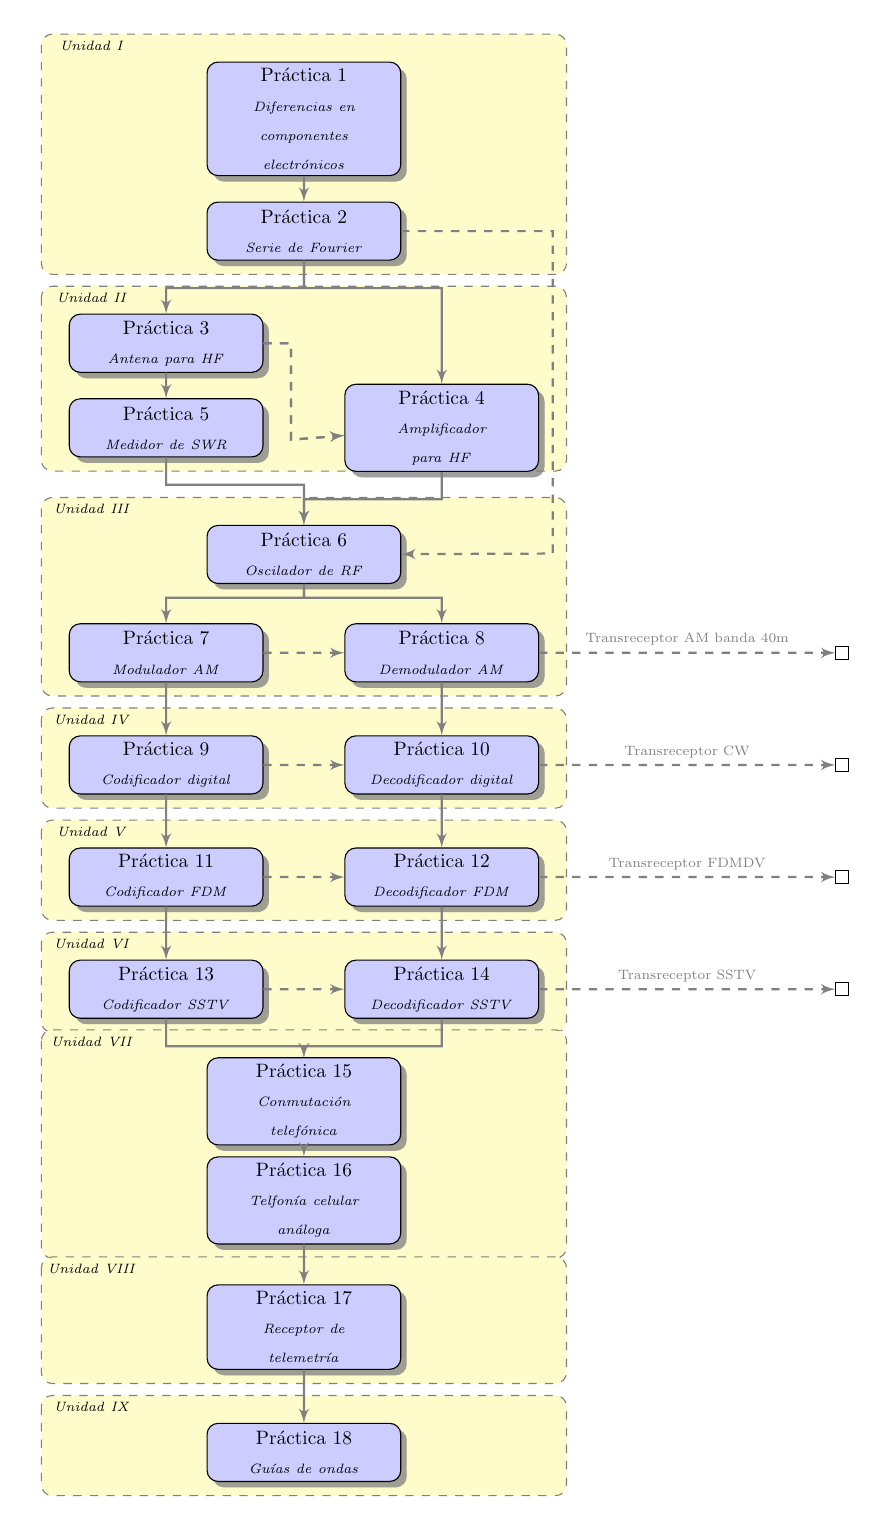
\begin{tikzpicture}[scale=0.7,transform shape]
 
  % Draw diagram elements
  \path \practica {1}{Diferencias en componentes electr\'onicos};
  \path (p1.south)+(0.0,-1.0) \practica{2}{Serie de Fourier};
  \path (p2.south)+(-2.5,-1.5) \practica{3}{Antena para HF};
  \path (p3.south)+(0.0,-1.0) \practica{5}{Medidor de SWR};
  \path (p3.south)+(5.0,-1.0) \practica{4}{Amplificador para HF};

  \path (p4.south)+(-2.5,-1.5) \practica{6}{Oscilador de RF};
  \path (p6.south)+(-2.5,-1.25) \practica{7}{Modulador AM};
  \path (p6.south)+(2.5,-1.25) \practica{8}{Demodulador AM};
  \path (p8.east)+(+5.5,0) node (ur1)[ur] {};

  \path (p7.south)+(0.0,-1.5) \practica{9}{Codificador digital};
  \path (p8.south)+(0.0,-1.5) \practica{10}{Decodificador digital};
  \path (p10.east)+(+5.5,0) node (ur2)[ur] {};
  \path (p9.south)+(0.0,-1.5) \practica{11}{Codificador FDM};
  \path (p10.south)+(0.0,-1.5) \practica{12}{Decodificador FDM};
  \path (p12.east)+(+5.5,0) node (ur3)[ur] {};
  \path (p11.south)+(0.0,-1.5) \practica{13}{Codificador SSTV};
  \path (p12.south)+(0.0,-1.5) \practica{14}{Decodificador SSTV};
  \path (p14.east)+(+5.5,0) node (ur4)[ur] {};
  \path (p14.south)+(-2.5,-1.5) \practica{15}{Conmutaci\'on telef\'onica};
  \path (p15.south)+(0.0,-1.0) \practica{16}{Telfon\'ia celular an\'aloga};
  \path (p16.south)+(0.0,-1.5) \practica{17}{Receptor de  telemetr\'ia}; 
  \path (p17.south)+(0.0,-1.5) \practica{18}{Gu\'ias de ondas};
     
  % Draw arrows between elements
  \path [line] (p1.south) -- node [above] {} (p2);

  \path [line] (p2.south) -- +(0.0,-0.5) -- +(-2.5,-0.5)
    -- node [above, midway] {} (p3);
  \path [line] (p3.south) -- node [above] {} (p5) ;
     
  \path [line] (p2.south) -- +(0.0,-0.5) -- +(+2.5,-0.5)
    -- node [above, midway] {} (p4);
  \path [linepart] (p3.east) -- +(+0.5,-0.0) -- +(+0.5,-1.75)
    -- node [left, midway] {} (p4);
  \path [linepart] (p3.east) -- +(+0.5,-0.0) -- +(+0.5,-1.75)
    -- node [left, midway] {} (p4);

  \path [line] (p4.south) -- +(0.0,-0.5) -- +(-2.5,-0.5)
    -- node [above, midway] {} (p6);
  \path [line] (p5.south) -- +(0.0,-0.5) -- +(+2.5,-0.5)
    -- node [above, midway] {} (p6);     
  \path [linepart] (p2.east) -- +(2.75,0.0) -- +(2.75,-5.85)
    -- node [right] {} (p6);
  \path [line] (p6.south) -- +(0.0,-0.25) -- +(-2.5,-0.25)
    -- node [above, midway] {} (p7);
  \path [line] (p6.south) -- +(0.0,-0.25) -- +(+2.5,-0.25)
    -- node [above, midway] {} (p8);
  \path [linepart] (p7.east) -- node [left] {} (p8);
  \transreceptor{p8}{AM banda 40m}{ur1}

  \path [line] (p7.south) -- node [above] {} (p9) ;
  \path [line] (p8.south) -- node [above] {} (p10) ;
  \path [linepart] (p9.east) -- node [left] {} (p10);
  \transreceptor{p10}{CW}{ur2}
  \path [line] (p9.south) -- node [above] {} (p11) ;
  \path [line] (p10.south) -- node [above] {} (p12) ;
  \path [linepart] (p11.east) -- node [left] {} (p12);
  \transreceptor{p12}{FDMDV}{ur3}

  \path [line] (p11.south) -- node [above] {} (p13) ;
  \path [line] (p12.south) -- node [above] {} (p14) ;
  \path [linepart] (p13.east) -- node [left] {} (p14);   
  \transreceptor{p14}{SSTV}{ur4}

  \path [line] (p14.south) -- +(0.0,-0.5) -- +(-2.5,-0.5)
    -- node [above, midway] {} (p15);
  \path [line] (p13.south) -- +(0.0,-0.5) -- +(+2.5,-0.5)
    -- node [above, midway] {} (p15);
  \path [line] (p15.south) -- node [above] {} (p16) ;     
  \path [line] (p16.south) -- node [above] {} (p17) ;
  \path [line] (p17.south) -- node [above] {} (p18) ;
   
  \background{p3}{p1}{p4}{p2}{I}
  \background{p3}{p3}{p4}{p5}{II}
  \background{p3}{p6}{p4}{p7}{III}
  \background{p3}{p9}{p4}{p10}{IV}
  \background{p3}{p11}{p4}{p12}{V}
  \background{p3}{p13}{p4}{p14}{VI}
  \background{p3}{p15}{p4}{p16}{VII}
  \background{p3}{p17}{p4}{p17}{VIII}
  \background{p3}{p18}{p4}{p18}{IX}
\end{tikzpicture}




















\begin{center}
\begin{tabular}{l|ll}
bla & set & vector\\ \hline

denk-450           
& 1.0 & 2.0\\
denk-450 ward         
& 1.0 & 5.0\\

bsd-500           
& 1.0 & 2.0\\
bsd-500 ward         
& 1.0 & 5.0

\end{tabular}
\end{center}



\begin{tikzpicture}[scale=  1,every node/.style={minimum size=1cm},on grid]
        
    %slanting: production of a set of n 'laminae' to be piled up. N=number of grids.
    

    %%%%%%%%%%%%%%%%%%%%%%%%%%%%%%%%%%%%%%%%%%%%%%%%%%%%%%%%%%%%%%%
    % 0 bottom layer
    %%%%%%%%%%%%%%%%%%%%%%%%%%%%%%%%%%%%%%%%%%%%%%%%%%%%%%%%%%%%%%%%
        
    \begin{scope}[
        yshift=0,every node/.append style={
            yslant=0.5,xslant=-1},yslant=0.5,xslant=-1
                     ]
        
        \draw[-latex,thick] (-0.17,2.5) node[right]{\includegraphics[width=5cm]{fig/lena.png}};
        \fill[white,fill opacity=.0] (0,0) rectangle (5,5);
        \draw[black,very thick] (0,0) rectangle (5,5);
        \draw[step=1.8mm, black] (0,0) grid (5,5);
    \end{scope}

    %%%%%%%%%%%%%%%%%%%%%%%%%%%%%%%%%%%%%%%%%%%%%%%%%%%%%%%%%%%%%%%
    % 1 layer
    %%%%%%%%%%%%%%%%%%%%%%%%%%%%%%%%%%%%%%%%%%%%%%%%%%%%%%%%%%%%%%%%
    
   \begin{scope}[
        yshift=100,every node/.append style={
            yslant=0.5,xslant=-1},yslant=0.5,xslant=-1
                     ]
        
        \draw[-latex,thick] (-0.17,2.5) node[right]{\includegraphics[width=5cm]{fig/lena.png}};
        \fill[white,fill opacity=.0] (0,0) rectangle (5,5);
        \draw[black,very thick] (0,0) rectangle (5,5);
        \draw[step=1.8mm, black] (0,0) grid (5,5);
    \end{scope}
        
     %%%%%%%%%%%%%%%%%%%%%%%%%%%%%%%%%%%%%%%%%%%%%%%%%%%%%%%%%%%%%%%
    % 2 layer
    %%%%%%%%%%%%%%%%%%%%%%%%%%%%%%%%%%%%%%%%%%%%%%%%%%%%%%%%%%%%%%%%
    
   \begin{scope}[
        yshift=200,every node/.append style={
            yslant=0.5,xslant=-1},yslant=0.5,xslant=-1
                     ]
        
        \draw[-latex,thick] (-0.17,2.5) node[right]{\includegraphics[width=5cm]{fig/lena.png}};
        \fill[white,fill opacity=.0] (0,0) rectangle (5,5);
        \draw[black,very thick] (0,0) rectangle (5,5);
        \draw[step=1.8mm, black] (0,0) grid (5,5);
    \end{scope}
        


    %%%%%%%%%%%%%%%%%%%%%%%%%%%%%%%%%%%%%%%%%%%%%%%%%%%%%%%%%%%%%%%
    % 0 bottom layer
    %%%%%%%%%%%%%%%%%%%%%%%%%%%%%%%%%%%%%%%%%%%%%%%%%%%%%%%%%%%%%%%%
    \draw[-latex,thick] (6.2,2) node[right]{$\mathsf{Grid Graph}$}
         to[out=180,in=90] (4,2);
         
         
         
    %%%%%%%%%%%%%%%%%%%%%%%%%%%%%%%%%%%%%%%%%%%%%%%%%%%%%%%%%%%%%%%
    % 1 layer
    %%%%%%%%%%%%%%%%%%%%%%%%%%%%%%%%%%%%%%%%%%%%%%%%%%%%%%%%%%%%%%%%
    
    \draw[-latex,thick] (6.2,5.5) node[right]{$\mathsf{Region adjacency graph 1}$}
         to[out=180,in=90] (4,5.5);

\end{tikzpicture}






































% We need layers to draw the block diagram
\pgfdeclarelayer{background}
\pgfdeclarelayer{foreground}
\pgfsetlayers{background,main,foreground}

% Define a few styles and constants
\tikzstyle{sensor}=[draw, fill=blue!20, text width=5em, 
    text centered, minimum height=2.5em]
\tikzstyle{ann} = [above, text width=5em]
\tikzstyle{naveqs} = [sensor, text width=6em, fill=red!20, 
    minimum height=12em, rounded corners]
\def\blockdist{2.3}
\def\edgedist{2.5}

\begin{tikzpicture}
    \node (naveq) [naveqs] {Navigation equations};
    % Note the use of \path instead of \node at ... below. 
    \path (naveq.140)+(-\blockdist,0) node (gyros) [sensor] {Gyros};
    \path (naveq.-150)+(-\blockdist,0) node (accel) [sensor] {Accelero-meters};
    
    % Unfortunately we cant use the convenient \path (fromnode) -- (tonode) 
    % syntax here. This is because TikZ draws the path from the node centers
    % and clip the path at the node boundaries. We want horizontal lines, but
    % the sensor and naveq blocks aren't aligned horizontally. Instead we use
    % the line intersection syntax |- to calculate the correct coordinate
    \path [draw, ->] (gyros) -- node [above] {$\vc{\omega}_{ib}^b$} 
        (naveq.west |- gyros) ;
    % We could simply have written (gyros) .. (naveq.140). However, it's
    % best to avoid hard coding coordinates
    \path [draw, ->] (accel) -- node [above] {$\vc{f}^b$} 
        (naveq.west |- accel);
    \node (IMU) [below of=accel] {IMU};
    \path (naveq.south west)+(-0.6,-0.4) node (INS) {INS};
    \draw [->] (naveq.50) -- node [ann] {Velocity } + (\edgedist,0) 
        node[right] {$\vc{v}^l$};
    \draw [->] (naveq.20) -- node [ann] {Attitude} + (\edgedist,0) 
        node[right] { $\mx{R}_l^b$};
    \draw [->] (naveq.-25) -- node [ann] {Horisontal position} + (\edgedist,0)
        node [right] {$\mx{R}_e^l$};
    \draw [->] (naveq.-50) -- node [ann] {Depth} + (\edgedist,0) 
        node[right] {$z$};
    
    % Now it's time to draw the colored IMU and INS rectangles.
    % To draw them behind the blocks we use pgf layers. This way we  
    % can use the above block coordinates to place the backgrounds   
    \begin{pgfonlayer}{background}
        % Compute a few helper coordinates
        \path (gyros.west |- naveq.north)+(-0.5,0.3) node (a) {};
        \path (INS.south -| naveq.east)+(+0.3,-0.2) node (b) {};
        \path[fill=yellow!20,rounded corners, draw=black!50, dashed]
            (a) rectangle (b);
        \path (gyros.north west)+(-0.2,0.2) node (a) {};
        \path (IMU.south -| gyros.east)+(+0.2,-0.2) node (b) {};
        \path[fill=blue!10,rounded corners, draw=black!50, dashed]
            (a) rectangle (b);
    \end{pgfonlayer}
\end{tikzpicture}


















\centering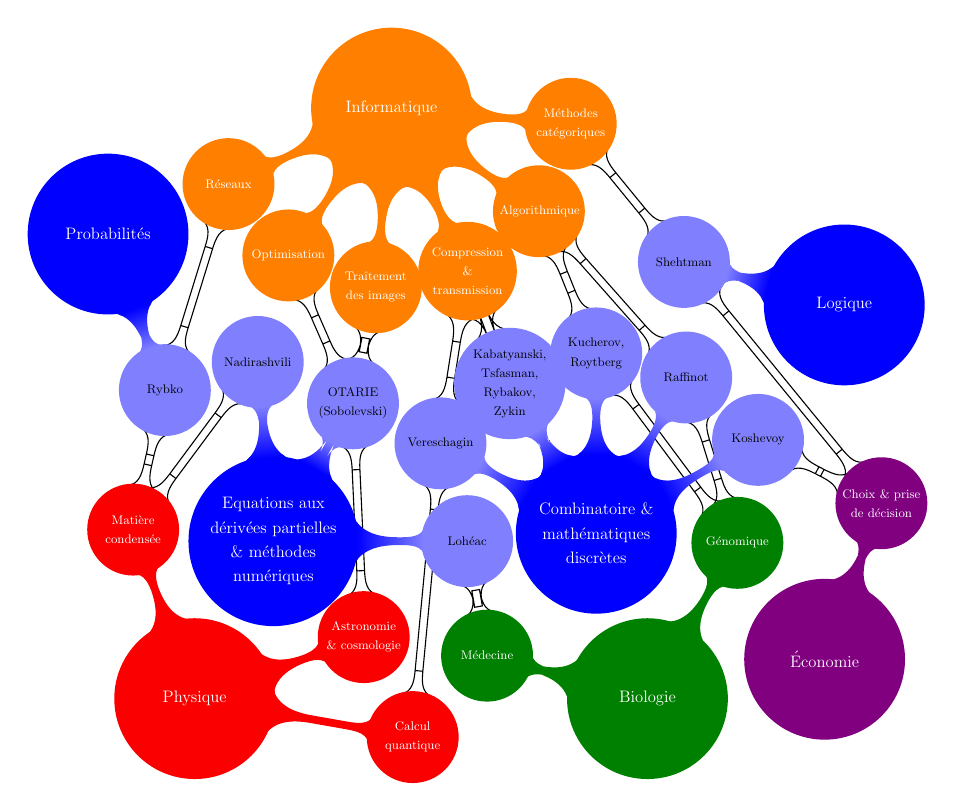
\begin{tikzpicture}[mindmap,scale=0.5, transform shape,
  level 1 concept/.append style={level distance=130,sibling angle=30},
  extra concept/.append style={color=blue!50,text=black}]
  % Applied area: computer science and its subfields

  \begin{scope}[mindmap, concept color=orange, text=white]
    \node [concept] {Informatique}[clockwise from=-5] 
      child {node [concept] (log) {M{\'e}thodes cat{\'e}goriques}}
      child {node [concept] (alg) {Algorithmique}}
      child {node [concept] (cod) {Compression \& transmission}}
      child {node [concept] (img) {Tra{\^i}tement des images}}
      child {node [concept] (opt) {Optimisation}}
      child {node [concept] (res) {R{\'e}seaux}};
  \end{scope}

  % Applied area: theoretical physics and its subfields

  \begin{scope}[mindmap, concept color=red,text=white]
    \node [concept] at (-5,-15) {Physique}
      child [grow=-10, level distance=160]
        {node [concept] (qin) {Calcul quantique}}
      child [grow=20] 
        {node [concept] (csm) {Astronomie \& cosmologie}}
      child [grow=110] 
        {node [concept] (mat) {Mati{\`e}re condens{\'e}e}};
  \end{scope}

  % Applied area: biology and its subfields

  \begin{scope}[mindmap, concept color=green!50!black,text=white]
    \node [concept] at (6.5,-15) {Biologie} 
      child [grow=165, level distance=120] 
        {node [concept] (med) {M{\'e}decine}}
      child [grow=60] 
        {node [concept] (gen) {G{\'e}nomique}};
  \end{scope}

  % Applied area: economics (one subfield)

  \begin{scope}[mindmap, concept color=violet, text=white]
    \node [concept] at (11,-14) {{\'E}conomie}
      child [grow=70, level distance=120] 
        {node [concept] (dec) {Choix \& prise de d{\'e}cision}};
  \end{scope}

  % Researchers listed by their main specialization in mathematics

  \begin{scope}[mindmap, concept color=blue]

    % Combinatorics and discrete mathematics 
    \node [concept, text=white] at (5.2,-10.8) 
      {Combinatoire \& math{\'e}matiques discr{\`e}tes} 
      [clockwise from=150]
      child [concept color=blue!50] {node [concept] (ver) {Vereschagin}}
      child [concept color=blue!50, level distance=125] 
        {node [concept] (kab) {Kabatyanski, Tsfasman, Rybakov, Zykin}}
      child [concept color=blue!50] 
        {node [concept] (kch) {Kucherov, Roytberg}}
      child [concept color=blue!50] {node [concept] (raf) {Raffinot}}
      child [concept color=blue!50, level distance=135]
        {node [concept] (ksh) {Koshevoy}};

    % Partial differential equations
    \node [concept, text=white] at (-3,-11) 
      {Equations aux d{\'e}riv{\'e}es partielles 
        \& m{\'e}thodes num{\'e}riques}
      child [concept color=blue!50, grow=0, level distance=140] 
        {node [concept] (lhc) {Loh{\'e}ac}}
      child [concept color=blue!50, grow=60, level distance=115] 
        {node [concept] (otr) {OTARIE (Sobolevski)}}
      child [concept color=blue!50, grow=95] {node [concept] (ndr) 
        {Nadirashvili}};

    % Probability
    \node [concept, text=white] at (-7.2,-3.2) {Probabilit{\'e}s}
      child [concept color=blue!50, grow=-70, level distance=120] 
        {node [concept] (rbk) {Rybko}};

    % Logic
    \node [concept, text=white] at (11.5,-5) {Logique}
      child [concept color=blue!50, grow=165, level distance=120] 
        {node [concept] (sht) {Shehtman}};
  \end{scope}

  % Connections of researchers to applied subfields

  \begin{pgfonlayer}{background}
    \draw [circle connection bar]
      (kab) edge (cod)
      (kch) edge (alg) edge (gen)
      (lhc) edge (med)
      (ksh) edge (dec)
      (ndr) edge (mat)
      (otr) edge (opt) edge (csm) edge (img)
      (raf) edge (alg) edge (gen)
      (rbk) edge (res) edge (mat)
      (sht) edge (log) edge (dec)
      (ver) edge (qin) edge (cod);
  \end{pgfonlayer}

\end{tikzpicture}


\newpage





% Below we mix an ordinary equation with TikZ nodes. Note that we have to
% adjust the baseline of the nodes to get proper alignment with the rest of
% the equation.
\begin{equation}
\omega_{e} = 
        \tikz[baseline]{\node[fill=blue!20,anchor=base] (te)        
            {$ f_{\epsilon}(X_{e}) $};
        } +
        \tikz[baseline]{\node[fill=red!20,anchor=base] (tuv)
            {$  d_{\nu}(X_u,X_v) $};
        } +   
        \tikz[baseline]{ \node[fill=green!20,anchor=base] (tr)
            {$r(|u|,|v|,|e|)$};  
        }
\end{equation}

\begin{itemize}
    \item Edge indicator:          \tikz\node [fill=blue!20,draw,circle] (ne) {};
        \begin{itemize}
         \item Gradient magnitude
         \item Eigenvalues of hessian
        \end{itemize}
    \item Node feature difference: \tikz\node [fill=red!20,draw,circle] (nuv) {};
       \begin{itemize}
         \item L1,L2
         \item Histogram differences ($\chi^2$,Earth movers distance)
       \end{itemize}
    \item Geometric regularizer:   \tikz\node [fill=green!20,draw,circle] (nr) {};
       \begin{itemize}
         \item Wards criterion \cite{ward_clustering}
         \item Log Ward criterion
         \item None 
      \end{itemize}
\end{itemize}

% Now it's time to draw some edges between the global nodes. Note that we
% have to apply the 'overlay' style.
%\begin{tikzpicture}[overlay]
%        \path[->] (ne) edge [bend right] (te);
%        \path[->] (nuv) edge [bend right] (tuv);
%        \path[->] (nr) edge [out=0, in=-90] (tr);
%\end{tikzpicture}



% -------------------------------------------------
% Set up a new layer for the debugging marks, and make sure it is on
% top
\pgfdeclarelayer{marx}
\pgfsetlayers{main,marx}
% A macro for marking coordinates (specific to the coordinate naming
% scheme used here). Swap the following 2 definitions to deactivate
% marks.
\providecommand{\cmark}[2][]{%
  \begin{pgfonlayer}{marx}
    \node [nmark] at (c#2#1) {#2};
  \end{pgfonlayer}{marx}
  } 
\providecommand{\cmark}[2][]{\relax} 


 

\cleardoublepage % Empty page before the start of the next part

%------------------------------------------------


\part{Software} % Second part of the thesis

% !TEX root = ../main.tex



\bigskip
\chapter{Vigra Graph Library} \label{ch:vigra_graph_lib}

Vigra \cite{software_vigra} is library for image processing and analysis.
Vigra provides customizable and genric algorithms and datastructures.
Vigra is capable of dealing with multi-dimensional images 
and many algorithms are implemented for arbitrary data types
and dimensions.
Vigra has a wide range of features from simple convolution filters, 
tensor based image processing to machine learning algorithms 
as decision trees.

To simplify the implementation of algorithms for images arbitrary 
dimension, vigra uses a grid graph which is capable of
dealing with any dimension.

Within this thesis we extend the concept graph based image processing
within vigra w.r.t. graphs of any structure.
We put main emphasis on extendability while keeping the usage very simple.


\section{Graph API's}\label{sec:graph_apis}

We strongly belief is is beneficial to use an existing API's for
graphs instead of inventing an own graph API for Vigra.
Coming up with a new API is not straight forward
since one might to think of any future use case this API.
In addition, users became accustomed with existing API's as 
the LEMON or Boost graph API.
Existing algorithms of a particular API can be reused if we stick
to that API.




\subsection{LEMON Graph API's}\label{sec:lemon_graph_apis}
    LEMON \citet{ software_lemon} 
    stand for  ``Library for Efficient Modeling and Optimization in Networks.''.
    It is an open source C++ library with algorithms and data structures 
    related to directed and undirected graphs.
    The extensive usage of templates make this library very flexible.
    While lemon provides a huge set of graph algorithms,
    we are mostly interested in the graph API itself.
    In the following we will give a brief overview of lemons graph 
    API and the related concepts.
    Explaining the complete lemon graph API in detail
    is beyond the scope of this thesis.
    Interested readers are referred to \citet{software_lemon}.
    We will only discuss the API for undirected graphs since any
    graph algorithm we implemented within this thesis
    will work on undirected graphs.

\subsubsection{Graph Items}
    Any undirected graph class fulfilling the lemon API needs to define 
    the following \emph{descriptor} types to represent the graph items.
    \begin{compactitem}
    \item \lstinline{Graph::Edge}
    \item \lstinline{Graph::Arc}
    \item \lstinline{Graph::Node}
    \end{compactitem}
    These \emph{descriptor} should be cheap types which can be copied
    and passed with almost no overhead.
    In addition, descriptor has an unique id
    \footnote{ unique id w.r.t. the item type. 
    Therefore  multiple  nodes cannot have the same id.
    The same holds line for edges and arcs.
    But there might be a node and edge which have the same id}.
    These id's can be accessed via \lstinline{Graph::id(Node)}, \lstinline{Graph::id(Edge)} and \lstinline{Graph::id(Arc)}.
    These id's can not only be dense but also sparse, which is very
    important for an efficient handling of grid graph edge ids.



\subsubsection{Iterators}

    Within lemon a very convenient mechanism is used to iterate over
    nodes, edges and arcs.
    A special constant \lstinline{INVALID} is used to determine if 
    an iterator reached the end.

    \begin{minipage}{\textwidth}\vspace{-0.75cm}\begin{lstlisting}[language=c++]
    // iterate over nodes
    for(Graph::NodeIt v(g); v!= lemon::INVALID; ++v){/*...*/}

    // iterate over edges
    for(Graph::EdgeIt e(g); e!= lemon::INVALID; ++e){/*...*/}

    // iterate over arcs
    for(Graph::ArcIt a(g); a!= lemon::INVALID; ++a){/*...*/}

    // use arcs to iterate over neighbor nodes
    for(Graph::OutArcIt a(g,n); a!= lemon::INVALID; ++a){
        const Node neighborNode = g.target(a);
        /*...*/
    }
    \end{lstlisting}\end{minipage}\vspace{0.5cm}

    Any iterator is convertible to the corresponding item which
    is iterated without using \lstinline{operator*()}.

\subsubsection{Map Concept}

    In lemon, graph classes store only the structure of the graph itself.
    All addition data for nodes, edges and arcs is stored 
    in \emph{maps}. 
    Any graph has default implementations for graph maps which
    can be accessed in the following way.

    \begin{minipage}{\textwidth}\vspace{-0.75cm}\begin{lstlisting}[language=c++]
    // edge map (for data as edge weights)
    Graph::EdgeMap<float> edgeMap(g); 

    // read and write data 
    for(Graph::EdgeIt e(g); e!= lemon::INVALID; ++e){
        // read
        const float val = edgeMap[*e];
        // write
        edgeMap[*e] = std::exp(-1.0*a);
    }

    // node map (for node related data as node labelings )
    Graph::NodeMap<usigned int> nodeMap(g);
    for(Graph::NodeIt v(g); v!= lemon::INVALID; ++v){
        // read
        const unsigned int val = nodeMap[*e];
        // write
        nodeMap[*e] = val+1;
    }
    \end{lstlisting}\end{minipage}\vspace{0.5cm}


    Custom maps can be implemented very easy:

    \begin{minipage}{\textwidth}\vspace{-0.75cm}\begin{lstlisting}[language=c++]
    template<class Graph>
    class ImplicitEdgeMap {
    public:
        typedef typename Graph::Edge Key;
        typedef double Value;
        Value operator[](Key edge) const { 
            Value a;
            /*...*/
            return a;
        }
    };
    \end{lstlisting}\end{minipage}\vspace{0.5cm}

\subsection{BOOST Graph API's}\label{sec:boost_graph_apis}
The Boost Graph Library (BGL)  \cite{software_bgl} is set of data structures and 
algorithms for graph related computations.
Since all algorithms are implemented within the LEMON graph interface, 
the BGL graph API will only be described briefly.
The graph API defined in the BGL is a collection of
free functions and graph traits which can be specialized for
any graph.




\subsection{VIGRA Graph API}

While the grid graph is implemented within the BGL and LEMON graph API,\
all algorithms implemented within this thesis will
use the LEMON graph API instead of the BGL 
for the following reason.
\todo{write reasons...}





\section{Implementation}\label{sec:vigra_graph_lib_impl}

The most important concept for graph based image processing
is the \emph{region adjacency graph} (RAG) (see \cref{fig:make_rag}).

A RAG is extracted from a labeled \emph{base graph}.
In the first step of graph based image processing, the base 
graph is usually a grid graph, and the labeling is a label image
as in \cref{fig:make_rag} .
To encode a RAG we need a undirected graph, 
and a mapping from the base graphs edges and nodes to the RAG 
needs to be stored.

The implementation of grid graphs is explained in \cref{sec:graphs_grid_graph}, 
a basic undirected graphs implementation will be discussed in \cref{sec:graphs_adjacency_list_graph}.
The implementation details of the \emph{region adjacency graph} concept will 
be given in  \cref{sec:graphs_rag}.

For hierarchical clustering we provide a specialized graph, named \emph{merge graph}.


To implemented structured clustering algorithms (see \cref{sec:rw_hc} we
need a graph which supports the contraction of edges.
Also a mechanism to merge node and edge features is needed.
Within \cref{sec:graphs_merge_graph} we propose  a very flexible
and concept for hierarchical clustering based on a specialized graph,
called \emph{merge graph}.


A generic set of algorithms which work on any graph
implemented within the VIGRA graph api is presented 
in \cref{sec:graph_graph_algorithms}.

While the core implementation of any algorithm is in C++
VIGRA provides python binding to make almost
any algorithm available in Python.
To provide a generic Python interface for any proposed
graph, we need to introduce a few concepts 
to make the python wrapped graph API very \emph{Pythonic}


\subsection{Graphs}


\subsubsection{Grid Graph} \label{sec:graphs_grid_graph}

\missingfigure{show grid graph here}

    \lstinline{vigra::GridGraph<DIM,DIRECTED_TAG>}

\subsubsection{Adjacency List Graph} \label{sec:graphs_adjacency_list_graph}


    \begin{minipage}{\textwidth}\vspace{-0.75cm}\begin{lstlisting}[language=c++]
    typedef AdjacencyListGraph Graph;

    // construct graph
    Graph g;

    // add nodes (id will be asigned automatically)
    Graph::Node n0 = g.addNode() 

    // add node with an explicit id
    Graph::Node n3 = g.addNode(3)

    // add edges from existing nodes
    Graph::Edge e0 = g.addEdge(n0,n1)

    // add edges and nodes simultaneous 
    Graph::Edge e1 = g.addEdge(2,3)

    // no parallel edges 
    Graph::Edge e2 = g.addEdge(2,3)
    assert(e1==e2)  
    \end{lstlisting}\end{minipage}\vspace{0.5cm}



\subsubsection{Region Adjacency Graph} \label{sec:graphs_rag}

To get a region adjacency graph (RAG), a labeled graph is needed.
The labeled graph will hereinafter be referred to as \emph{base graph} 
$G_{\text{base}}$
of the RAG.

To map edges and nodes from the base graph


\subsubsection{Merge Graph} \label{sec:graphs_merge_graph}
To implemented structured clustering algorithms (see \cref{???}) we
need a graph which supports the contraction of edges.
Also a mechanism to merge node and edge features is needed.
Experiments suggest that the edge contraction is more expensive
than feature merging an can even be a bottleneck for huge 3D data 
(see \cref{???} ).
Therefore it is crucial to implemented the MergeGraph (MG) very carefully.
\begin{figure}
    \centering
    \includegraphics[width=0.35\textwidth]{fig/contraction.pdf}

    \addtocontents{lof}{%
        \vspace{1cm}
        \protect\centerline{%
            \protect\includegraphics[width=\lofthumbsize,height=\lofthumbsize,keepaspectratio=true]{fig/contraction.pdf} 
        } 
    }%

    %\addtocontents{lof}{%
    %    $\vcenter to \lofthumbsize{\vss%
    %        \hbox to \lofthumbsize {
    %            \hss \protect \includegraphics[width=.075\linewidth]{fig/contraction.pdf} \hss
    %        }
    %    \vss}$%
    %    \quad
    %    \ignorespaces
    %}%
    \caption[Schematic edge contraction]{ Schematic edge contraction: Node $u$ and $v$ is merged into node $w$.
        Note the gray node $n$ which is connected to $u$ and $v$.
        After the contraction, edges $\{ n,u\}$ and $\{ n,v\}$ are also merged into 
        a single edge $\{ n, w\}$ 
    }
    \label{fig:figlabel}
\end{figure}


   

\begin{center}
    \begin{tikzpicture}
        \umlclass[template=Graph]{MergeGraphAdpator}
        {
            \\// union find data structures                     \\
            - edgeUfd               : IterablePartiton          \\
            - nodeUfd               : IterablePartiton          \\ 
            - nodesAdjacency        : AdjacencySetVector        \\

            \\// callbacks                                      \\
            - mergeNodeCallBacks    : MergeNodeCallBackVector   \\
            - mergeEdgeCallBack     : MergeEdgeCallBackVector   \\
            - eraseEdgeCallBack     : EraseEdgeCallBackVector   \\
        }
        {
            \\// LEMON API for undirected graphs                \\
                $\ldots$                                        \\
            \\// register callbacks                             \\ 
            + registerMergeNodeCallBack(f : MergeNodeCallBack)  \\
            + registerMergeEdgeCallBack(f : MergeEdgeCallBack)  \\
            + registerEraseEdgeCallBack(f : EraseEdgeCallBack)  \\

            \\// modify graph                                   \\
            + contractEdge(edge : Edge)     : Node              \\

            \\// find representatives                           \\
            + reprNode(node : Node)         : Node              \\
            + reprEdge(edge : Edge)         : Edge              \\ 

            \\// get base graph                                 \\
            + graph()                       : Graph             \\
        } 
    \end{tikzpicture}
\end{center}

\begin{center}
    \begin{tikzpicture}
        \umlclass[template=MergeGraph]{ClusterOperatorInterface}
        {

        }
        {
            \\// contract next edge and get weight              \\
            + contractionEdge(edge : Edge)         : Edge       \\ 
            + contractionWeight(edge : Edge)       : Edge       \\
            \\// get base graph                                 \\
            + mergeGraph()                  : MergeGraph        \\
        } 
    \end{tikzpicture}
\end{center}

\begin{center}
    \begin{tikzpicture}
        \umlclass[template=ClusterOperator]{HierarchicalClustering}
        {

        }
        {
            + cluster()                     : void        \\
            + reprLabels(nodeMap : NodeMap) : void        \\      
        } 
    \end{tikzpicture}
\end{center}


   We propose and implemented the following design:
   \begin{compactitem}
       \item  A base graph is attached to a merge graph  and  a merge graph will
            always ``view'' to
       \item  Union find data structure for nodes
       \item  Union find data structure for edges
   \end{compactitem}



   \lstinline{vigra::MergeGraphAdaptor<DIM,DIRECTED_TAG>}


\subsection{Graph Algorithms} \label{sec:graph_graph_algorithms}

    \subsubsection{Multicut}

    \subsubsection{Hierarchical Clustering}

    \subsubsection{Mst Algorithms}

    \subsubsection{Watershed Algorithms}

    \subsubsection{Smoothing Algorithms}





\section{Python}




\begin{flushright}{\slshape    
(1) Beautiful is better than ugly. \\ \label{cit:line_a}
(2) Explicit is better than implicit. \\ \label{cit:line_b}
(3) Simple is better than complex. \\
(4) Complex is better than complicated. \\
(5) Flat is better than nested. \\
(6) Sparse is better than dense. \\
(7) Readability counts. \\
(8) Special cases aren't special enough to break the rules. \\
(9) Although practicality beats purity. \\
(10) Errors should never pass silently. \\
(11) Unless explicitly silenced. \\
(12) In the face of ambiguity, refuse the temptation to guess. \\
(13) There should be one-- and preferably only one --obvious way to do it. \\
(14) Although that way may not be obvious at first unless you're Dutch. \\
(15) Now is better than never. \\
(16) Although never is often better than *right* now. \\
(17) If the implementation is hard to explain, it's a bad idea. \\
(18) If the implementation is easy to explain, it may be a good idea. \\
(19) Namespaces are one honking great idea -- let's do more of those! } \\ \medskip
--- The Zen of Python
\end{flushright}
\captionof{figure}{ 
    The Zen of Python
}\label{fig:zen_of_python}






\subsection{Graph Maps}

On the python side, we want node-maps, edge-maps and arc-maps to be stored 
as numpy arrays for several reasons.
Numpy arrays are the standard for storing multidimensional data in python.
The fast C implementation and the highly vectorized API of numpy makes it very easy to write 
fast python code within a few lines.
Virtually any python user will be familiar with the numpy API and therefore it 
seems to be natural to store graph maps within numpy arrays.

In addition VIGRA provides an mechanism to pass numpy arrays to C++.
Therefore no new mechanism needs to be implemented to transfer graph
maps from python to C++.
This will not only simplify writing extension for the new VIGRA graph API,
but also it will reduce the glue code since we can use well tested existing
solutions.

New algorithms might be implemented in pure python with a mix of
existing numpy functions and new functions provided within VIGRA's graph API.
As a proof of concept we implemented ??? in pure python with VIGRA's
fresh graph API in \cref{???}.


\subsubsection{Intrinsic Graph Shape}

Each graph has an \emph{intrinsic node map shape} 
and an \emph{intrinsic edge map shape} and 
These intrinsic shape and dimensions are used to use 
numpy arrays with the best fitting dimension and shape.
For a 2D grid graph the node map should also be a 2D dimensional array.
because in this way an usual image can be used as an node map.
To access the  intrinsic shapes of node and edge maps 
we use a small trait class with default implementations
for unknown graphs.
The default implementation is given below:

\begin{minipage}{\textwidth}\vspace{-0.75cm}\begin{lstlisting}[language=c++]
template<class GRAPH>
class IntrinsicGraphShape{
private:
    typedef GRAPH Graph;
    typedef typename vigra::MultiArray<1,int>::difference_type DiffType1d;
    typedef typename Graph::index_type  index_type;
public:
    typedef typename Graph::Node Node ;
    typedef typename Graph::Edge Edge ;
    typedef typename  Graph::Arc  Arc ;

    typedef DiffType1d IntrinsicNodeMapShape;
    typedef DiffType1d IntrinsicEdgeMapShape;
    typedef DiffType1d  IntrinsicArcMapShape;

    static IntrinsicNodeMapShape intrinsicNodeMapShape(const Graph & g){
        return IntrinsicNodeMapShape(g.maxNodeId()+1);
    }
    static IntrinsicEdgeMapShape intrinsicEdgeMapShape(const Graph & g){
        return IntrinsicEdgeMapShape(g.maxEdgeId()+1);
    }
    static IntrinsicArcMapShape intrinsicArcMapShape(const Graph & g){
        return  IntrinsicArcMapShape(g.maxArcId()+1);
    }

    static const unsigned int IntrinsicNodeMapDimension=1;
    static const unsigned int IntrinsicEdgeMapDimension=1;
    static const unsigned int IntrinsicArceMapDimension=1;
};
\end{lstlisting}\end{minipage}\vspace{0.5cm}



\subsubsection{Numpy Arrays To LEMON Maps}


On the C++ side, numpy arrays are stored in MultiArrayViews.
Since the API of MultiArrayViews \cite{software_vigra_multiarray_api} does
not implemented the API  of LEMON graph maps (e.g. node-maps, edge-maps and arc-maps), 
a thin wrapper is used to convert the arrays to LEMON conform maps.
These wrappers can be accessed via \lstinline{PyNodeMapTraits<Graph,T>::Array} and 
\lstinline{PyNodeMapTraits<Graph,T>::Map}. 


In the following we will give a brief example how to pass numpy arrays to C++
and convert them to LEMON conform graph maps.

Assuming we need a function which does something with node features as normalization.
On the python side we want to have the following signature:

\lstinline{result=vigra.graphs.normNodeFeat(graph,nodeFeatures=nodeFeatures,out=None)}.

The function should work on single band node features and multi band node features
(an arbitrary number of channels, but the same for all nodes).
There should be a single C++ function which can be used to export
\lstinline{normNodeFeat} for any graph within VIGRA's graph API. 




\begin{minipage}{\textwidth}

To archive this we propose the following design:
On the C++ side we use a function  which
is has two templates , one for the graph, and one for the value type.
A prototypical implementation is given below.

\begin{minipage}{\textwidth}\vspace{-0.75cm}\begin{lstlisting}[language=c++]
template<class Graph,class T>
NumpyAnyArray normNodeFeat(
    const Graph & g,
    const typename PyNodeMapTraits<Graph,T >::Array & nodeFeaturesInArray,
    typename PyNodeMapTraits<Graph,T>::Array  outArray 
){
    // reshape out 
    // - last argument (outArray) will be reshaped if empty,
    // - and #channels is taken from second argument (nodeFeaturesIn) 
    reshapeNodeMapIfEmpty(g,nodeFeaturesIn,outArray);

    // numpy arrays => lemon maps 
    // featuresInMap and outMap fulfill
    // the concept of LEMON NODE MAPS
    typename PyNodeMapTraits<Graph,T >::Map featuresInMap(g,nodeFeaturesInArray);
    typename PyNodeMapTraits<Graph,T >::Map outMap(g,outArray);


    /* call code using LEMON API*/

    // return out as numpy array
    return outArray;
}
\end{lstlisting}\end{minipage}\vspace{0.5cm}

The template \lstinline{T} can be instantiated with scalars as \lstinline{float}, an explicit single band scalar as \lstinline{Singleband<float>}
or a multi band type as \lstinline{Multiband<float>}.

\lstinline{PyNodeMapTraits<Graph,T >::Array} will select the correct \lstinline{vigra::NumpyArray<DIM,VALUE_TYPE>} w.r.t.
the templates \lstinline{Graph} and \lstinline{T}.

The output array will be reshaped with the corrected number of channels by calling \lstinline{reshapeNodeMapIfEmpty}.
Equivalent functions exist for edge maps.

\lstinline{PyNodeMapTraits<Graph,T >::Map} is the corresponding LEMON conform  node map 
which is a cheap view to an numpy array. 
\end{minipage}


\begin{minipage}{\textwidth}
To make the function above available in python
we need to write wrapper code with \lstinline{boost::python}.
We will export the function for single band floats and multi band floats.

\begin{minipage}{\textwidth}\vspace{-0.75cm}\begin{lstlisting}[language=c++]
// single-band float32
boost::python::def(
    "normNodeFeat",
     &normNodeFeat<Graph,float>,
    (
        boost::python::arg("graph"),
        boost::python::arg("nodeFeatures"),
        boost::python::arg("out")=boost::python::object() // None
    )
);

// multi-band float32
boost::python::def(
    "normNodeFeat",
     &normNodeFeat<Graph,Multiband<float> >,
    (
        boost::python::arg("graph"),
        boost::python::arg("nodeFeatures"),
        boost::python::arg("out")=boost::python::object() // None
    )
);
\end{lstlisting}\end{minipage}\vspace{0.5cm}

\end{minipage}


On the python side we can call the function as desired.
The array which stores the result of this
function can be preallocated and passed explicitly.

\begin{minipage}{\textwidth}\vspace{-0.75cm}\begin{lstlisting}[language=Python]
// with automatically allocated outFeatures
outFeatures = vigra.graphs.normNodeFeat(graph,nodeFeatures)

// with explicitly given outFeatures
// - here we assume single band features
outFeatures2 = vigra.graphs.graphMap(graph,item='node',dtype=np.float32)
outFeatures2 = vigra.graphs.normNodeFeat(graph,nodeFeatures,out=outFeatures2)


// with multiband node features 
// - here we assume multi band features
//   with 3 channels per node
outFeatures2 = vigra.graphs.graphMap(graph,item='node',dtype=np.float32,channels=3)
outFeatures2 = vigra.graphs.normNodeFeat(graph,nodeFeatures,out=outFeatures2)
\end{lstlisting}\end{minipage}\vspace{0.5cm}




\subsection{Graph Hierarchy}
    
Explain the very nice workflow  

%\include{Chapters/Chapter02} % Chapter 2
%\include{Chapters/Chapter03} % Chapter 3
%\include{Chapters/Chapter04} % Chapter 4 - empty template

\part{Experiments}



%----------------------------------------------------------------------------------------
%	THESIS CONTENT - APPENDICES
%----------------------------------------------------------------------------------------

\appendix

\part{Appendix} % New part of the thesis for the appendix

%\include{Chapters/Chapter0A} % Appendix A
%\include{Chapters/Chapter0B} % Appendix B - empty template

%----------------------------------------------------------------------------------------
%	POST-CONTENT THESIS PAGES
%----------------------------------------------------------------------------------------

\cleardoublepage% Bibliography

\label{app:bibliography} % Reference the bibliography elsewhere with \autoref{app:bibliography}

\manualmark
\markboth{\spacedlowsmallcaps{\bibname}}{\spacedlowsmallcaps{\bibname}} 
\refstepcounter{dummy}

\addtocontents{toc}{\protect\vspace{\beforebibskip}} % Place the bibliography slightly below the rest of the document content in the table of contents
\addcontentsline{toc}{chapter}{\tocEntry{\bibname}}

\bibliographystyle{plainnat}

\bibliography{Bibliography} % Bibliography
\cleardoublepage% Colophon (a brief description of publication or production notes relevant to the edition)

\pagestyle{empty}

\hfill

\vfill

\pdfbookmark[0]{Colophon}{colophon}

\section*{Colophon}

This document was typeset using the typographical look-and-feel \texttt{classicthesis} developed by Andr\'e Miede. The style was inspired by Robert Bringhurst's seminal book on typography ``\emph{The Elements of Typographic Style}''. \texttt{classicthesis} is available for both \LaTeX\ and \mLyX: 

\begin{center}
\url{http://code.google.com/p/classicthesis/}
\end{center}

\noindent Happy users of \texttt{classicthesis} usually send a real postcard to the author, a collection of postcards received so far is featured here: 

\begin{center}
\url{http://postcards.miede.de/}
\end{center}
 
\bigskip

\noindent\finalVersionString % Colophon
\cleardoublepage% Declaration

\refstepcounter{dummy}
\pdfbookmark[0]{Declaration}{declaration} % Bookmark name visible in a PDF viewer

\chapter*{Declaration} % Declaration section text

\thispagestyle{empty}

Put your declaration here.
\bigskip
 
\noindent\textit{\myLocation, \myTime}

\smallskip

\begin{flushright}
\begin{tabular}{m{5cm}}
\\ \hline
\centering\myName, \today \\
\end{tabular}
\end{flushright}
 % Declaration

%----------------------------------------------------------------------------------------

\end{document}
